\documentclass[12pt,a4paper,oneside, most]{report}

\usepackage[a4paper, top=30mm, bottom=30mm, left=30mm, right=25mm]{geometry}
%Penggunaan bahasa
\usepackage[bahasa]{babel}
%Library penggunaan gambar
\usepackage{graphicx}
%\usepackage{subcaption}
\usepackage{siunitx}
%Pengaturan Judul
\usepackage[utf8]{inputenc}
%\usepackage[utf8x]{inputenc}
%\usepackage{import}
% Menambahkan dummy text, bullet, atau rumus
\usepackage{blindtext}
\usepackage{lipsum}
% Pengaturan bab
\usepackage{sectsty}
\usepackage{titlesec}
% Pengelolaan Daftar Pustaka
%\usepackage{natbib}
%\usepackage[nottoc]{tocbibind}
% Pengaturan Sub judul gambar atau tabel
\usepackage{subcaption}
% Pengaturan tabel
\usepackage{multirow}
\usepackage[table,xcdraw]{xcolor}
%Pengaturan Enumerate
\usepackage{enumitem}
%pengaturan judul gambar
\usepackage[labelsep=quad]{caption}
%pengaturan tabel berlanjut di halaman berikutnya
\usepackage{longtable}
\usepackage{amssymb}
\usepackage{amsmath}
\usepackage{appendix}
\usepackage{soul}
%pengaturan rata kiri kanan
\usepackage{ragged2e}
% Pengaturan spasi section
\titlespacing{\section}{0pt}{\parskip}{\parskip}

% Pengaturan left caption
%\captionsetup[table]{singlelinecheck=off}
\usepackage[font=normalsize,labelfont=bf,tableposition=top]{caption}
\usepackage{physics}
\usepackage[utf8]{inputenc}

\usepackage{booktabs} % To thicken table lines
\usepackage{float}

\usepackage{booktabs}
\usepackage{multirow}
\usepackage[table,xcdraw]{xcolor}

%Pengaturan kotak kosong
\usepackage{tcolorbox}
% Pengaturan Judul di Tengah
\titleformat{\chapter}[display]{\LARGE\bfseries\centering}{\MakeUppercase\chaptertitlename\ \thechapter}{-5pt}{\Large\bfseries\uppercase}
\titlespacing*{\chapter}{0pt}{-20pt}{20pt}
% Pengaturan ukuran huruf section
\titleformat*{\section}{\Large\bfseries}
\titleformat*{\subsection}{\large\bfseries}
\titleformat*{\subsubsection}{\large\bfseries}
\titleformat*{\paragraph}{\large\bfseries}
\titleformat*{\subparagraph}{\large\bfseries}

%Blankpage%
\def\blankpage{%
    \clearpage%
    \thispagestyle{empty}%
    \addtocounter{page}{-1}%
    \null%
    \clearpage}
%Pengaturan Roman dan Arabic untuk Chapter, Section, Subsection
\renewcommand{\thechapter}{\arabic{chapter}}
\renewcommand{\thesection}{\arabic{chapter}.\arabic{section}}
\renewcommand{\thesubsection}{\thesection.\arabic{subsection}}
\renewcommand{\thefigure}{\arabic{chapter}.\arabic{figure}}
\renewcommand{\thetable}{\arabic{chapter}.\arabic{table}}


%% Mengganti nama Bab menjadi Percobaan
\addto\captionsbahasa{\renewcommand{\chaptername}{BAB}}
\addto\captionsbahasa{\renewcommand{\bibname}{DAFTAR PUSTAKA}}

% Pengaturan Nama BAB di TOC
\usepackage[titles]{tocloft}
\setlength{\cftchapnumwidth}{0pt}
\setlength{\cftbeforechapskip}{\baselineskip}
\renewcommand{\cftchappresnum}{\chaptername\ }
\renewcommand{\cftchapaftersnum}{.}
\renewcommand{\cftchapaftersnumb}{\newline}
\renewcommand{\cftchapdotsep}{\cftdotsep}

\graphicspath{{././figures/}}

\tolerance=1
\emergencystretch=\maxdimen
\hyphenpenalty=10000
\hbadness=10000

\setlength{\parskip}{0.5em}


%\usepackage{xcolor}
\definecolor{tssteelblue}{RGB}{70,130,180}
\definecolor{tsorange}{RGB}{255,138,88}
\definecolor{tsblue}{RGB}{23,74,117}
\definecolor{tsforestgreen}{RGB}{21,122,81}
\definecolor{tsyellow}{RGB}{255,185,88}
\definecolor{tsgrey}{RGB}{200,200,200}
\definecolor{codegreen}{rgb}{0,0.6,0}
\definecolor{codegray}{rgb}{0.5,0.5,0.5}
\definecolor{codepurple}{rgb}{0.58,0,0.82}
\definecolor{backcolour}{rgb}{0.95,0.95,0.92}
\definecolor{lightgray}{rgb}{0.95,0.95,0.95}
\definecolor{lightyellow}{rgb}{0.98, 0.98, 0.7}

\usepackage{tcolorbox}
\usepackage{algorithm}
\usepackage{algpseudocode}
\usepackage{listings}
\tcbuselibrary{listings,breakable}
\usepackage{amsthm}

\newenvironment{boxprogram}
{\begin{tcolorbox}
        [enhanced jigsaw,breakable,pad at break*=1mm,
            colback=backcolour,boxrule=0pt,frame hidden,
            borderline west={1.5mm}{-2mm}{tsblue}]}
        {\end{tcolorbox}}

\newtheoremstyle{styleprogram}
{0pt}{0pt}{\normalfont}{0pt}{\small\bf\sffamily\color{black}}{\\}{0.25em}
{\small\sffamily\color{tsblue}\thmname{#1}
    \nobreakspace\thmnumber{#2}
    \thmnote{\nobreakspace\the\thm@notefont\sffamily\bfseries\color{black} (#3)}}

%\newtheoremstyle{styleprogram}
%{0pt}{0pt}{\normalfont}{0pt}{\small\bf\sffamily\color{black}}{\\}{0.25em}
%{\small\sffamily\color{tsblue}\thmname{#1}
% \nobreakspace\thmnumber{\@ifnotempty{#1}{}\@upn{#2}}
% \thmnote{\nobreakspace\the\thm@notefont\sffamily\bfseries\color{black} (#3)}}

\theoremstyle{styleprogram}
\newtheorem{envprogram}{Program}[chapter]

\newenvironment{program}
{\begin{boxprogram}\begin{envprogram}}
            {\end{envprogram}\end{boxprogram}}


\lstdefinestyle{mystyle}{
    backgroundcolor=\color{backcolour},
    commentstyle=\color{codegreen},
    keywordstyle=\color{magenta},
    numberstyle=\tiny\color{codegray},
    stringstyle=\color{codepurple},
    basicstyle=\ttfamily\scriptsize,
    breakatwhitespace=false,
    breaklines=false,
    captionpos=b,
    keepspaces=true,
    numbers=left,
    numbersep=5pt,
    showspaces=false,
    showstringspaces=false,
    showtabs=false,
    tabsize=2
}

\lstset{style=mystyle}

\usepackage{makecell}
\usepackage{hyperref}
\AtBeginDocument{\RenewCommandCopy\qty\SI}

\AtBeginDocument{\RenewCommandCopy\qty\SI}

\begin{document}
\pagenumbering{roman}
\begin{titlepage}
	\vspace*{-2cm}
	\begin{table}[!ht]
		\begin{flushright}
			\begin{tabular}{|c|}
				\hline
				\begin{tabular}[c]{@{}c@{}}RISET KERJASAMA INDUSTRI\end{tabular} \\ \hline
			\end{tabular}
		\end{flushright}
	\end{table}
	\vspace{0.3cm}
	\begin{center}
		%\vspace*{1cm} 
		\Large
		\textbf{LAPORAN PENELITIAN}\\
		\vspace{0.3cm}
		TENTANG \\
		\normalsize
		\vspace{0.3cm}
		\textbf{Pengembangan Infrastruktur IoT Campus Testbed (C-IoT-TB) untuk Penelitian Jaringan Sensor Nirkabel dan Aplikasi IoT Terapan}\\
		\vspace{0.5cm}

		Penelitian ini dibiayai dengan Dana DIPA\\
		Nomor	: SP DIPA 023.18.2.677606/2024\\
		Polteknik Negeri Malang\\
		dengan Surat Perjanjian Nomor : 5583/PL2.1/HK/2024\\
		\vspace{1cm}
		Oleh:\\
		\textbf{Indrazno Siradjuddin, ST., MT., PhD.}\\
		NIDN. 0024067406\\
		\textbf{Prof. Dr. Budhy Setiawan, B.SEET., MT}\\
		NIDN: 0009046405\\
		\textbf{Gillang Al Azhar, S.S.T., M.Tr.T}\\
		NIDN: 0022069501\\
		\textbf{Zakiyah Amalia, ST., M.Tr.T}\\
		NIDN. 0014019405\\
		\vspace{1cm}
		
\includegraphics[width=0.35\linewidth]{polinema.png}
		\vspace{2.5cm}

		\large
		\textbf{POLITEKNIK NEGERI MALANG\\
			15 Oktober 2024}

	\end{center}
\end{titlepage}


\pagenumbering{arabic}
%Identitas dan Uraian Umum Penelitian
\addcontentsline{toc}{chapter}{Identitas dan Uraian Umum Penelitian}
\title{Identitas}
\begin{center}
	\large \textbf{IDENTITAS DAN URAIAN UMUM PENELITIAN}
\end{center}
\vspace{0.5cm}
\textbf{1. Judul Penelitian:}\\
{DISAIN DAN IMPLEMENTASI PERANGKAT PEMBELAJARAN SISTEM OTOMASI INDUSTRI DENGAN MODEL PREDICTIVE CONTROL: STUDI KASUS CART-INVERTED PENDULUM} \\

\hspace{-0.6cm}\textbf{2. Tim Peneliti:}


\begin{table}[h!]
	\centering
	\resizebox{\textwidth}{!}{%
		\begin{tabular}{|c|l|c|c|c|c|}
			\hline
			\textbf{No}&
			\multicolumn{1}{c|}{\textbf{Nama}} &
			\textbf{Jabatan}&
			\textbf{\begin{tabular}[c]{@{}c@{}}Bidang \\ Keahlian\end{tabular}}&
			\textbf{Jurusan}&
			\textbf{\begin{tabular}[c]{@{}c@{}}Alokasi waktu\\ (Jam/Minggu)\end{tabular}}\\ \hline
			1 &
			\begin{tabular}[c]{@{}l@{}}Indrazno Siradjuddin, \\ S.T., M.T., Ph.D.\end{tabular} &
			\begin{tabular}[c]{@{}c@{}}Ketua Peneliti\\ Dosen \\ DIV-PSTE\end{tabular} &
			Robotika &
			\begin{tabular}[c]{@{}c@{}}Teknik\\ Elektro\end{tabular} &
			10 \\ \hline
			2 &
			\begin{tabular}[c]{@{}l@{}}Prof. Dr. Budhy Setiawan, B.SEET., MT, \end{tabular} &
			\begin{tabular}[c]{@{}c@{}}Anggota Peneliti \\ Dosen \\ DIV-PSTE\end{tabular} &
			\begin{tabular}[c]{@{}c@{}}Mekatronika\end{tabular} &
			\begin{tabular}[c]{@{}c@{}}Teknik\\ Elektro \end{tabular} &
			10 \\ \hline
			3 &
			\begin{tabular}[c]{@{}l@{}}Gillang Al Azhar, S.S.T., M.Tr.T \end{tabular} &
			\begin{tabular}[c]{@{}c@{}}Anggota Peneliti \\ Dosen \\ DIII-PSTE \end{tabular} &
			\begin{tabular}[c]{@{}c@{}}Robotika \end{tabular} &
			\begin{tabular}[c]{@{}c@{}}Teknik\\ Elektro \end{tabular} &
			10 \\ \hline
			4 &			
			\begin{tabular}[c]{@{}l@{}}Zakiyah Amalia, ST., M.Tr.T\end{tabular} &
			\begin{tabular}[c]{@{}c@{}}Pembantu Peneliti \\ Dosen \\ DIV-PSTM\end{tabular} &
			\begin{tabular}[c]{@{}c@{}}Sistem Kontrol \end{tabular} &
			\begin{tabular}[c]{@{}c@{}}Teknik\\ Mesin\end{tabular} &
			10 \\ \hline
			5 &			
			\begin{tabular}[c]{@{}l@{}}Ida Lailatul Fitria \end{tabular} &
			\begin{tabular}[c]{@{}c@{}}Mahasiswa \\ MTTE \end{tabular} &
			\begin{tabular}[c]{@{}c@{}}Sistem kontrol \\ dan Robotika\end{tabular} &
			\begin{tabular}[c]{@{}c@{}}Teknik\\ Elektro\end{tabular} &
			10 \\ \hline
			6&			
			\begin{tabular}[c]{@{}l@{}}Febby Ayu Salsabillah \end{tabular} &
			\begin{tabular}[c]{@{}c@{}}Mahasiswa \\ MTTE  \end{tabular} &
			\begin{tabular}[c]{@{}c@{}}Sistem kontrol \\ dan Robotika\end{tabular} &
			\begin{tabular}[c]{@{}c@{}}Teknik\\ Elektro\end{tabular} &
			10 \\ \hline
			8&			
			\begin{tabular}[c]{@{}l@{}}Dimas Adi Prayoga \end{tabular} &
			\begin{tabular}[c]{@{}c@{}}Mahasiswa \\ MTTE \end{tabular} &
			\begin{tabular}[c]{@{}c@{}}Sistem kontrol \\ dan Robotika\end{tabular} &
			\begin{tabular}[c]{@{}c@{}}Teknik\\ Elektro\end{tabular} &
			10 \\ \hline
            9&			
			\begin{tabular}[c]{@{}l@{}}Arif Anwar Rosyidin \end{tabular} &
			\begin{tabular}[c]{@{}c@{}}Mahasiswa \\ MTTE \end{tabular} &
			\begin{tabular}[c]{@{}c@{}}Sistem kontrol \\ dan Robotika\end{tabular} &
			\begin{tabular}[c]{@{}c@{}}Teknik\\ Elektro\end{tabular} &
			10 \\ \hline
		\end{tabular}%
	}
\end{table}


\hspace{-0.6cm}\textbf{3. Objek Penelitian (jenis material yang akan diteliti dan segi penelitian):}\\
Obyek penelitian adalah produk cart-inverted pendulum yang dilengkapi dengan sensor, embedded system serta software untuk implementasi MPC secara realtime \\

\hspace{-0.6cm}\textbf{4. Masa Pelaksanaan:}\\
8 bulan\\

\hspace{-0.6cm}\textbf{5. Biaya:}\\
Rp 40.000.000,00\\

\hspace{-0.6cm}\textbf{6. Lokasi Penelitian:}\\
Laboratorium MTTE dan Workshop di tempat Mitra \\

\hspace{-0.6cm}\textbf{7. TKT Awal: 4}\hspace{1cm} \textbf{TKT akhir yang akan dihasilkan: 6}\\

\hspace{-0.6cm}\textbf{8. Grup Riset:}\\
Intelligent Systems and Robotics (ISaR)\\

\hspace{-0.6cm}\textbf{9. Instansi lain yang terlibat:}\\
Mitra\\

\hspace{-0.6cm}\textbf{10. Temuan yang ditargetkan:}
Prototipe yang dapat digunakan untuk mendemonstrasikan sistem kontrol MPC secara realtime \\

%\vspace{0.5cm}

\hspace{-0.6cm}\textbf{11. Kontribusi mendasar pada suatu bidang ilmu
(uraikan tidak lebih dari 50 kata, tekankan pada gagasan fundamental dan orisinal yang akan mendukung pengembangan IPTEKSB):}\\
Penelitian akan menghasilkan inovasi sebuah prototipe produk peralatan LAB sistem kontrol yang dapat digunakan untuk melakukan eksperimen-eksperimen disain algoritma sistem control secara real-time, dalam penelitian ini difokuskan pada implementasi Model Predictive Control.\\

\hspace{-0.6cm}\textbf{12. Jurnal ilmiah yang menjadi sasaran (tuliskan nama terbitan berkala ilmiah internasional bereputasi, nasional terakreditasi, atau nasional tidak terakreditasi dan tahun rencana publikasi): }\\
Luaran publikasi berupa artikel untuk seminar internasional terindeks Scopus, ICVEE 2024.\\

\hspace{-0.6cm}\textbf{13. Rencana luaran HKI, buku, purwarupa atau luaran lainnya yang ditargetkan, tahun rencana perolehan atau penyelesaiannya:}\\
Luaran KI berupa kode program komputer implementasi MPC untuk cart-inverted pendulum secara realtime 
\newpage

\addcontentsline{toc}{chapter}{Daftar Isi}
\newpage
\setlength{\parskip}{0.5em}
\tableofcontents
\pagebreak
%\setlength{\parskip}{1em}
\listoffigures
\addcontentsline{toc}{chapter}{Daftar Gambar}
%\setlength{\parskip}{1em}
\listoftables
\addcontentsline{toc}{chapter}{Daftar Tabel}
\newpage
\addcontentsline{toc}{chapter}{Ringkasan}
\title{Ringkasan}
\begin{center}
	\large \textbf{RINGKASAN}
\end{center}

Penelitian dengan judul “Disain Dan Implementasi Perangkat Pembelajaran Sistem Otomasi Industri Dengan Model Predictive Control: Studi Kasus Cart-Inverted Pendulum” berupaya mengembangkan sebuah prototipe sistem kontrol berbasis Model Predictive Control (MPC) yang dapat diaplikasikan dalam sebuah laboratorium sistem kontrol. Pada tahap awal penelitian, asumsi baseline adalah bahwa teknologi yang ada telah mencapai TKT level 4, yang menggambarkan adanya literatur dan pemahaman konseptual yang cukup kuat terkait MPC. Namun, perlu adanya pengembangan lebih lanjut agar teknologi ini dapat ditingkatkan hingga mencapai TKT level 6 di akhir penelitian. Mencapai TKT level 6 dalam kesiapan teknologi akan berarti adanya implementasi prototipe MPC yang berfungsi penuh dan teruji dengan baik. Hal ini akan melibatkan pengembangan perangkat keras yang solid serta pengoptimalan algoritma pendukungnya. Secara terperinci, proses penelitian akan dimulai dengan pemilihan komponen perangkat keras yang tepat untuk implementasi MPC. Pengembangan perangkat lunak untuk mendukung algoritma kontrol juga akan menjadi fokus yang krusial. Keselarasan antara perangkat keras dan perangkat lunak, serta optimalisasi kinerja sistem secara keseluruhan akan menjadi bagian penting dalam pembangunan prototipe ini.  Seperti yang telah disebutkan sebelumnya, output yang diharapkan dari penelitian ini sangat komprehensif. Pertama-tama, prototipe cart-inverted pendulum dengan kontrol MPC yang berfungsi penuh akan menjadi pencapaian kunci, menandai sebuah langkah maju dalam penggabungan teori kontrol yang rumit dengan implementasi dunia nyata. Selain itu, artikel ilmiah yang dikembangkan dalam penelitian ini diharapkan akan diterima untuk presentasi pada konferensi internasional terindeks seperti IEEE (ICVE2024). Hal ini akan menjadi suatu pencapaian signifikan yang dapat memberi pengakuan dan kontribusi pengetahuan yang substansial dalam bidang sistem kontrol. Selain itu, penelitian memasukkan juga pengembangan dokumen Feasibility Study serta dokumen Implementation Arrangement dan Hak Cipta berupa KI program komputer. Ini menunjukkan keseriusan dalam menjelajahi potensi komersialisasi prototipe hasil penelitian ini. Estimasi mengenai perhitungan biaya, analisis pasar, serta proyeksi pendapatan akan menjadi bagian utama dalam dokumen feasibility study. Dokumen arrangement implementasi akan memberikan panduan terinci tentang bagaimana prototipe ini dapat diterapkan secara komersial serta menjelaskan langkah demi langkah yang diperlukan untuk mencapai tujuan tersebut Selain dari aspek pengembangan teknologi dan akademis, penelitian ini juga memiliki dampak yang signifikan pada pendidikan dan pengembangan teknologi di bidang sistem kontrol. Prototipe dan temuan yang dilaporkan dapat bermanfaat bagi siswa, peneliti, dan industri sebagai sumber inspirasi, referensi, dan mungkin juga sebagai produk konkret di pasar.
\vspace*{1cm}

\noindent KATA KUNCI

Pemodelan, sistem dinamik, kontrol, MPC, Cart-Inverted Pendulum
\chapter{Pendahuluan}
\section{Latar Belakang}

\section{Rumusan Masalah}
Perumusan masalah dalam penelitian adalah langkah penting yang mengarahkan fokus studi secara spesifik. Untuk penelitian dengan judul "Disain Dan Implementasi Perangkat Pembelajaran Sistem Otomasi Industri Dengan Model Predictive Control: Studi Kasus Cart-Inverted Pendulum", permasalahan dapat dirumuskan sebagai berikut:


\section{Batasan Masalah}
Untuk memfokuskan penelitian pada pengembangan perangkat keras dengan menggunakan sistem tertanam seperti Arduino atau ESP32 dan software untuk program sistem tertanam tersebut, batasan masalah harus dijelaskan secara eksplisit. Berikut adalah beberapa batasan masalah yang bisa ditetapkan:



\section{Tujuan Penelitian}
Tujuan dari penelitian ini adalah untuk merancang dan mengimplementasikan sebuah perangkat pembelajaran yang berfokus pada aplikasi Model Predictive Control (MPC) dalam sistem dinamik khususnya Cart-Inverted Pendulum menggunakan platform mikrokontroler seperti Arduino atau ESP32. Upaya ini bertujuan untuk memfasilitasi pemahaman konseptual yang lebih baik dan penerapan praktis MPC bagi mahasiswa dan peneliti, dengan menyediakan alat praktikum yang mampu mengilustrasikan tantangan nyata sistem kontrol non-linear dan tak stabil. Perangkat pembelajaran ini diharapkan dapat menjadi alat efektif dalam mengatasi kesenjangan antara teori kontrol yang kompleks dengan aplikasi dunia nyata, sekaligus meningkatkan kualitas pendidikan teknik kontrol dan mendukung kurikulum yang ada dengan cara yang inovatif dan interaktif.

\begin{table}[!htb]
    %\centering
    \caption{Luaran Penelitian}
    \label{tab:my-table}
    \resizebox{\textwidth}{!}{%
        \begin{tabular}{|c|l|c|}
            \hline
            \textbf{No} & \multicolumn{1}{c|}{\textbf{Jenis Luaran}}                                    & \textbf{Indikator Capaian *)} \\ \hline
            \multicolumn{3}{|l|}{Luaran Wajib}                                                                                          \\ \hline
            1           & \begin{tabular}[c]{@{}l@{}}IPTEKSB berupa prototype\end{tabular}              & Ada                           \\ \hline
            2           & Feasibility study (analisis kebutuhan pelanggan, kondisi pasar, dan teknis)   & Ada                           \\ \hline
            3           & Dokumen uji yang dikeluarkan/ telah divalidasi Ada oleh lembaga yang kompeten & Ada                           \\ \hline
            4           & Dokumen Implementation Arrangement (IA)                                       & Ada                           \\ \hline
            \multicolumn{3}{|l|}{Luaran Tambahan}                                                                                       \\ \hline
            1           & Prosiding seminar internasional terindeks (SCOPUS, IEEE)                      & Presented                     \\ \hline
        \end{tabular}%
    }
\end{table}

\section{Manfaat Penelitian}


\section{Luaran Penelitian}
Luaran penelitian dapat dilihat pada Tabel~\ref{tab:my-table}.







\chapter{Profil Mitra Industri}
\begin{figure}[!htb]
    \centering
    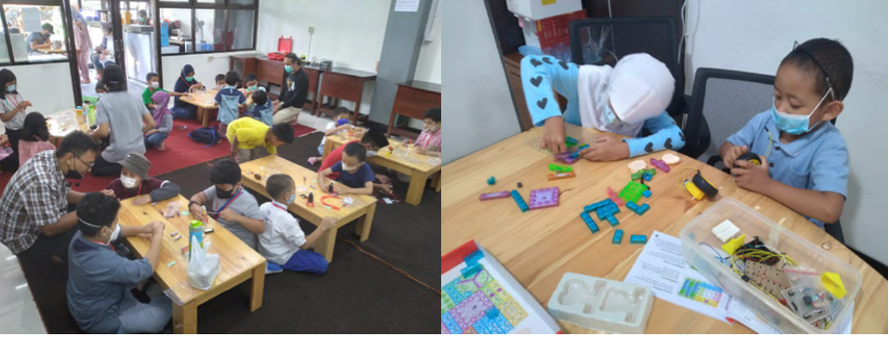
\includegraphics[width=0.7\textwidth]{figures/KegiatanKiddo.png}
    \caption{Kegiatan di Kido Robot}
    \label{fig:kegiatankiddo}
\end{figure}
\begin{figure}[!htb]
    \centering
    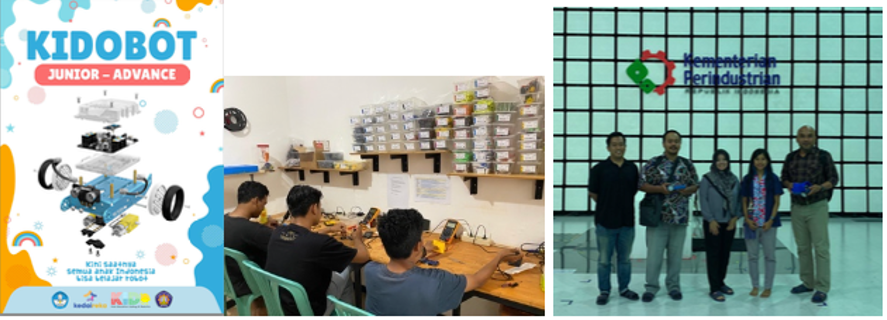
\includegraphics[width=0.7\textwidth]{figures/ProdukWorkshopKiddo.png}
    \caption{Produk dan Workshop di Kido Robot}
    \label{fig:produkkiddo}
\end{figure}
Kido Robot adalah perusahaan yang berfokus pada produksi dan pelatihan modul edukasi robotika. Inisiatif Kido Robot yang dimulai sejak 2014, memiliki misi untuk menyiapkan sumber daya manusia dalam menghadapi ekonomi digital, khususnya di bidang teknologi robotika. Antara lain dengan melakukan pelatihan private, kursus rutin grup dan workshop robotik. Kido Robot juga berkolaborasi dengan sekolah-sekolah dan ikatan guru dalam pengembangan dan pelatihan robotika. Gambar~\ref{fig:kegiatankiddo}  adalah gambaran kegiatan di Kiddo Robot. Gambar~\ref{fig:produkkiddo} adalah gambaran salah satu produk, situasi workshop dan kerjasama yang pernah dilakukan dengan Politeknik Negeri Malang. 

Dedikasi bahwa platform pendidikan dalam aliran berkelanjutan dari fase prasekolah ke fase dewasa harus disediakan untuk kreativitas dan daya pikir mengembangkan pendidikan yang akan menjadi dasar untuk menumbuhkan bakat di setiap bidang, Kido Robot memfasilitasi berbagai platform pendidikan untuk segala usia. Khususnya, alat pendidikan berkualitas baik untuk robot, pengkodean, dan STEM memungkinkan pembelajaran bakat yang efektif. 

Kido Robot telah banyak bekerja sama dengan sekolah-sekolah di area Kota Malang, diantaranya sekolah Andalusia Kids, Tweddle Land, Al Muttaqien, dan lain sebagainya. Tidak hanya dalam kegiatan ekstrakulikuler saja namun dalam berkolaborasi membuat modul belajar robotika juga. Sehingga dapat tercipta modul-modul edukasi yang baik. Selain bekerja sama dengan sekolah, Kido Robot juga menjalin kerjasama kegiatan dengan taman atau lokasi permainan anak. Misi yang dicapai adalah bukan hanya untuk menjadikan siswa-siswa menjadi juara, tapi lebih daripada hal tersebut adalah membuat siswa-siswa senang belajar utamanya dalam hal teknologi dan membuat mereka siap dalam menghadapi perkembangan teknologi yang signifikan. 

\chapter{Tinjauan Pustaka}
\section{Embedded systems dan IoT}
Istilah IoT (Internet of Things) merupakan istilah yang relatif baru tetapi mengacu pada penggunaan lama yang disebut Machine-to-Machine.
Machine-to-Machine (M2M) adalah sekumpulan teknologi jaringan kabel atau nirkabel yang memungkinkan pertukaran informasi secara otomatis antar sistem tanpa intervensi manusia. IoT hanyalah visi yang lebih luas dari M2M, di mana perangkat tidak hanya berasal dari dunia industri, tetapi juga dari penggunaan publik umum.
Pasar IoT terus berkembang pesat di seluruh dunia. Perkembangan pesat ini mendorong pemain baru untuk mengusulkan teknologi baru pada setiap tahap: pengembangan perangkat keras, cakupan konektivitas, dan layanan cloud (misalnya, platform penyimpanan atau visualisasi data).
IoT sering disajikan sebagai revolusi industri baru, dan pemasaran sering menjanjikan bahwa semua kasus penggunaan bersifat "smart": smart building, smart city, smart healthcare, dll. Namun, membuat sesuatu menjadi “smart” tidak selalu mudah dan banyak protokol yang ada.
\subsection{Embedded System}
Embedded systems adalah sistem komputasi khusus yang dirancang untuk menjalankan fungsi tertentu dalam sistem yang lebih besar. Sistem ini biasanya ditandai dengan integrasinya ke dalam perangkat yang dikendalikan, operasi real-time, dan keterbatasan sumber daya (misalnya, daya pemrosesan, memori, dan konsumsi energi yang terbatas). Embedded systems dapat ditemukan dalam berbagai aplikasi, mulai dari elektronik konsumen (misalnya, smartphone, perangkat rumah pintar) hingga otomasi industri (misalnya, robotika, kontrol proses).
Dalam konteks IoT, embedded systems memainkan peran penting sebagai "things" yang mengumpulkan dan memproses data dari lingkungan. Sistem ini sering mencakup sensor, aktuator, dan antarmuka komunikasi yang memungkinkannya berinteraksi dengan perangkat lain dan cloud. Desain dan pengembangan embedded systems untuk aplikasi IoT memerlukan pertimbangan hati-hati terhadap faktor-faktor seperti konektivitas, interoperabilitas, keamanan, dan manajemen daya.
Secara umum, sistem elektronik dapat dikarakterisasi berdasarkan konsumsi daya, daya komputasi, ukuran, dan harga. Dalam kasus khusus embedded systems yang digunakan dalam IoT, kita dapat memberikan bobot berikut pada masing-masing karakteristik:
Meskipun tentu ada pengecualian terhadap definisi sederhana ini, kita mengasumsikan bahwa, dibandingkan dengan sistem elektronik lainnya, embedded systems yang digunakan dalam IoT memiliki:
\begin{enumerate}
    \item Konsumsi daya rendah (Low-power consumption)
    \item Daya komputasi rendah (Low computing power)
    \item Ukuran kecil (A small size)
    \item Harga rendah (A low price)
\end{enumerate}
Karakteristik-karakteristik ini sering saling terkait. Misalnya, ukuran kecil biasanya menyiratkan konsumsi daya rendah dan harga rendah. Demikian pula, konsumsi daya rendah sering menyiratkan daya komputasi rendah. Desain embedded systems sering merupakan pertukaran (trade-off) antara karakteristik-karakteristik ini, tergantung pada aplikasi dan kebutuhan spesifik.
\subsection{Protokol nirkabel IoT}
Protokol nirkabel IoT dapat diklasifikasikan ke dalam tiga kategori utama berdasarkan jangkauan dan laju data: protokol jangkauan pendek, jangkauan menengah, dan jangkauan jauh.
\begin{enumerate}
    \item Protokol jangkauan pendek: Protokol ini dirancang untuk komunikasi pada jarak pendek, biasanya dalam beberapa meter. Protokol ini umum digunakan untuk jaringan area pribadi (PANs) dan aplikasi otomasi rumah. Contoh protokol jangkauan pendek termasuk Bluetooth, Zigbee, dan Wi-Fi.
    \item   Protokol jangkauan menengah: Protokol ini dirancang untuk komunikasi pada jarak sedang, biasanya hingga beberapa ratus meter. Protokol ini umum digunakan untuk jaringan area lokal (LANs) dan aplikasi otomasi industri. Contoh protokol jangkauan menengah termasuk Wi-Fi, Z-Wave, dan Thread.
    \item Protokol jangkauan jauh: Protokol ini dirancang untuk komunikasi pada jarak jauh, biasanya beberapa kilometer atau lebih. Protokol ini umum digunakan untuk jaringan area luas (WANs) dan aplikasi smart city. Contoh protokol jangkauan jauh termasuk LoRaWAN, Sigfox, dan NB-IoT.
    \item Protokol jangkauan sangat jauh: Protokol ini dirancang untuk komunikasi pada jarak yang sangat jauh, biasanya puluhan kilometer. Protokol ini umum digunakan untuk aplikasi yang memerlukan jangkauan ekstrem, seperti pemantauan lingkungan dan pertanian cerdas. Contoh protokol jangkauan sangat jauh termasuk Long Range (LoRa) dan Weightless.
\end{enumerate}


Setiap protokol ini memiliki kelebihan dan kekurangan masing-masing, dan pemilihan protokol tergantung pada kebutuhan spesifik aplikasi IoT, seperti jangkauan, laju data, konsumsi daya, dan biaya.
Sigfox dan LoRaWAN dianggap sebagai protokol dengan jangkauan sangat jauh dan daya sangat rendah. Jenis jaringan ini semuanya disebut sebagai Low Power Wide Area Network (LPWANs). Dalam penelitian ini, kami fokus pada LoRaWAN (Long Range Wide Area Network) yang merupakan standar jangkauan jauh yang menggunakan laju data rendah dengan kebutuhan konsumsi daya rendah.
\section{Ikhtisar Dasar-dasar dan Arsitektur LoRaWAN}
LoRaWAN adalah protokol Low Power Wide Area Network (LPWAN) yang dirancang untuk mendukung komunikasi jarak jauh, daya rendah, dan laju data rendah untuk aplikasi Internet of Things (IoT). Dikembangkan dan dipelihara oleh LoRa Alliance, protokol ini mendefinisikan lapisan Media Access Control (MAC) yang beroperasi di atas lapisan fisik yang disediakan oleh modulasi LoRa. Sejak rilis awalnya pada Januari 2015, LoRaWAN telah berkembang melalui beberapa versi spesifikasi, dengan LoRaWAN 1.0.4 dan 1.1 mewakili iterasi stabil terbaru pada saat penulisan.
Bagian ini memberikan ikhtisar teknis singkat tentang dasar-dasar LoRaWAN, termasuk karakteristik utamanya, arsitektur, model komunikasi, mekanisme keamanan, dan domain aplikasi khas.
\subsection{Karakteristik Utama LoRaWAN}
LoRaWAN menampilkan beberapa fitur utama yang membuatnya sangat cocok untuk penyebaran IoT:
\begin{enumerate}
    \item \textbf{Jangkauan Jauh}: Jangkauan komunikasi hingga 10+ km di lingkungan pedesaan dan 2–5 km di lingkungan perkotaan yang padat dapat dicapai, tergantung pada medan dan kondisi interferensi.
    \item \textbf{Konsumsi Daya Rendah}: Perangkat akhir dapat beroperasi selama 5–10 tahun atau lebih dengan satu baterai karena pengoptimalan siklus tugas (duty cycling) dan mode tidur.
    \item \textbf{Komunikasi Aman}: Kerahasiaan dan integritas data end-to-end dijamin melalui enkripsi berbasis AES simetris.
    \item \textbf{Komunikasi Dua Arah}: Protokol ini mendukung pengiriman pesan uplink (perangkat-ke-server) dan downlink (server-ke-perangkat).
    \item \textbf{Skalabilitas}: Jaringan LoRaWAN dapat mendukung jutaan perangkat per gateway karena skema akses berbasis ALOHA dan mekanisme Adaptive Data Rate (ADR).
    \item \textbf{Dukungan Geolokasi}: LoRaWAN memungkinkan geolokasi perangkat tanpa GPS melalui teknik time difference of arrival (TDOA) menggunakan beberapa gateway.
    \item \textbf{Adaptive Data Rate (ADR)}: Protokol ini secara dinamis menyesuaikan laju data dan daya transmisi berdasarkan kualitas link untuk mengoptimalkan kapasitas jaringan dan masa pakai baterai.
    \item \textbf{Standardisasi Global}: LoRaWAN distandardisasi oleh LoRa Alliance, memastikan interoperabilitas di seluruh perangkat dan jaringan di seluruh dunia.
\end{enumerate}
\subsection{Batasan Laju Data dan Payload}
LoRaWAN dioptimalkan untuk transmisi data kecil dan tidak sering. Batasan utama meliputi:
\begin{enumerate}
    \item \textbf{Ukuran Payload}: Berkisar antara 51 hingga 242 byte per pesan, tergantung pada peraturan regional dan laju data yang dipilih.
    \item \textbf{Laju Data}: Bervariasi antara 0,3 kbps hingga 50 kbps, ditentukan oleh spreading factor (SF) dan konfigurasi bandwidth.
    \item \textbf{Frekuensi Pesan}: Perangkat biasanya dirancang untuk mengirimkan 1–100 pesan per hari.
    \item \textbf{Duty Cycle}: Tunduk pada batasan peraturan nasional (misalnya, 1\% di Eropa berdasarkan peraturan ETSI).
    \item Spreading factor adalah parameter transmisi kritis yang menukar laju data dengan jangkauan komunikasi dan ketahanan: spreading factor yang lebih tinggi (misalnya, SF12) memungkinkan komunikasi jarak jauh dengan biaya throughput yang lebih rendah, sedangkan spreading factor yang lebih rendah (misalnya, SF7) mendukung laju data yang lebih tinggi pada jarak yang lebih pendek.
\end{enumerate}
\subsection{Domain Aplikasi Khas}
LoRaWAN banyak diadopsi dalam skenario yang menuntut masa pakai baterai yang panjang, cakupan luas, efisiensi biaya, dan pertukaran data minimal. Kasus penggunaan representatif meliputi:
\begin{enumerate}
    \item \textbf{Pertanian Cerdas}: Pemantauan kelembaban tanah, pelacakan kesehatan tanaman, manajemen ternak.
    \item \textbf{Pemantauan Lingkungan}: Pemantauan kualitas udara, pemantauan ketinggian air, stasiun cuaca.
    \item \textbf{Gedung Cerdas}: Kontrol HVAC, manajemen pencahayaan, deteksi hunian.
    \item \textbf{Pelacakan Aset}: Manajemen armada, pelacakan inventaris, pemantauan rantai dingin.
    \item \textbf{Kota Cerdas}: Kontrol pencahayaan jalan, pemantauan lalu lintas dan parkir, manajemen limbah.
    \item \textbf{Pertanian}: Pemantauan kelembaban tanah, otomasi irigasi, pelacakan ternak.
    \item \textbf{Rantai Pasok dan Logistik}: Pelacakan aset, pemantauan rantai dingin, manajemen inventaris.
    \item \textbf{Utilitas}: Pengukuran pintar untuk air, gas, dan listrik; deteksi kebocoran dan perusakan.
    \item \textbf{IoT Industri}: Pemantauan kondisi, perawatan prediktif, pemantauan lingkungan.
\end{enumerate}
\subsection{LoRa vs. LoRaWAN}
Penting untuk membedakan antara LoRa dan LoRaWAN:
\begin{enumerate}
    \item \textbf{LoRa} adalah teknik modulasi lapisan fisik berpaten yang berbasis Chirp Spread Spectrum (CSS). LoRa mengkodekan data menggunakan pulsa chirp yang dimodulasi frekuensi linear, menawarkan anggaran link (link budget) yang tinggi dan ketahanan terhadap fading multipath dan pergeseran Doppler.
    \item \textbf{LoRaWAN} adalah protokol lapisan MAC yang mendefinisikan bagaimana perangkat yang diaktifkan LoRa mengakses jaringan, menyusun pesan, mengelola sesi, dan memastikan keamanan. LoRaWAN menstandarkan perilaku perangkat di berbagai penyebaran heterogen dan memungkinkan interoperabilitas.
\end{enumerate}
Dengan demikian, LoRa menyediakan mekanisme transmisi fisik, sedangkan LoRaWAN mengatur aturan komunikasi tingkat jaringan.
\subsection{Arsitektur Jaringan}
Jaringan LoRaWAN standar terdiri dari empat komponen utama:
\begin{enumerate}
    \item \textbf{End Devices}: Node sensor atau aktuator yang menghasilkan atau menerima data aplikasi. Mereka berkomunikasi secara nirkabel menggunakan modulasi LoRa.
    \item \textbf{Gateways}: Transceiver multi-saluran dan multi-modem yang menerima pesan uplink dari end devices dan meneruskannya ke Network Server melalui backhaul (misalnya, Ethernet, seluler). Gateway juga meneruskan pesan downlink dari server ke end devices.
    \item \textbf{Network Server (LNS)}: Perangkat lunak terpusat yang bertanggung jawab atas manajemen jaringan, termasuk deduplikasi pesan, kontrol adaptive data rate (ADR), dan routing.
    \item \textbf{Application Server}: Memproses data lapisan aplikasi yang didekripsi dan berinteraksi dengan layanan pengguna akhir atau dashboard.
\end{enumerate}
\subsection{Alur Pesan}
LoRaWAN menggunakan topologi star-of-stars, di mana end devices berkomunikasi langsung dengan beberapa gateway. Alur pesan dapat dirangkum sebagai berikut:
\subsubsection{Komunikasi Uplink}
Pesan uplink berasal dari end devices dan dikirim melalui udara menggunakan skema akses acak berbasis ALOHA—tidak diperlukan pemasangan berpasangan dengan gateway tertentu. Semua gateway dalam jangkauan radio menerima pesan dan meneruskannya ke Network Server. Server melakukan deduplikasi dengan menyimpan hanya satu salinan dari penerimaan yang berulang dan kemudian memisahkan payload lapisan jaringan dan lapisan aplikasi.
\subsubsection{Komunikasi Downlink}
Pesan downlink diprakarsai oleh Network Server atau Application Server dan dijadwalkan untuk transmisi selama jendela penerimaan yang telah ditentukan (RX1 dan RX2) setelah uplink. Network Server memilih gateway yang sesuai untuk mengirimkan pesan berdasarkan kualitas link dan batasan waktu.
\subsection{Model Keamanan}
LoRaWAN menggunakan skema enkripsi kunci simetris dua lapis untuk memastikan pemisahan perhatian antara fungsi jaringan dan aplikasi:
\begin{enumerate}
    \item \textbf{Network Session Key (NwkSKey)}: Mengenkripsi perintah MAC dan memastikan integritas payload lapisan jaringan. Hanya diketahui oleh end device dan Network Server.
    \item \textbf{Application Session Key (AppSKey)}: Mengenkripsi data aplikasi. Dibagikan secara eksklusif antara end device dan Application Server.
\end{enumerate}
Kunci sesi ini diturunkan dari kunci root selama prosedur join (baik Over-the-Air Activation—OTAA—atau Activation-by-Personalization yang telah ditentukan sebelumnya—ABP). Kunci sesi diputar ulang saat bergabung kembali ke jaringan, meningkatkan kerahasiaan ke depan (forward secrecy).
\subsection{The Things Stack}
The Things Stack adalah implementasi open-source kelas enterprise dari LoRaWAN Network Server yang mengintegrasikan fungsi Network Server dan Application Server. The Things Stack mendukung onboarding aman, manajemen, dan pemantauan jutaan perangkat LoRaWAN dalam skala besar. Dengan mengabstraksi detail protokol tingkat rendah, The Things Stack memungkinkan penyebaran solusi LoRaWAN siap produksi yang cepat di berbagai vertikal.
LoRaWAN merupakan solusi yang kuat, distandardisasi, dan dapat diskalakan untuk penyebaran IoT berbasis LPWAN. Kombinasi kemampuan jangkauan jauh, efisiensi energi, keamanan yang kuat, dan kemampuan beradaptasi dengan peraturan telah mendorong adopsi global di infrastruktur cerdas, pertanian, logistik, dan otomasi industri. Memahami arsitektur berlapisnya—mulai dari modulasi fisik (LoRa), protokol MAC (LoRaWAN), hingga perangkat lunak jaringan (misalnya, The Things Stack)—sangat penting untuk merancang dan menyebarkan sistem IoT yang andal.
\section{Arsitektur LoRaWAN}
\begin{figure}
    \centering
    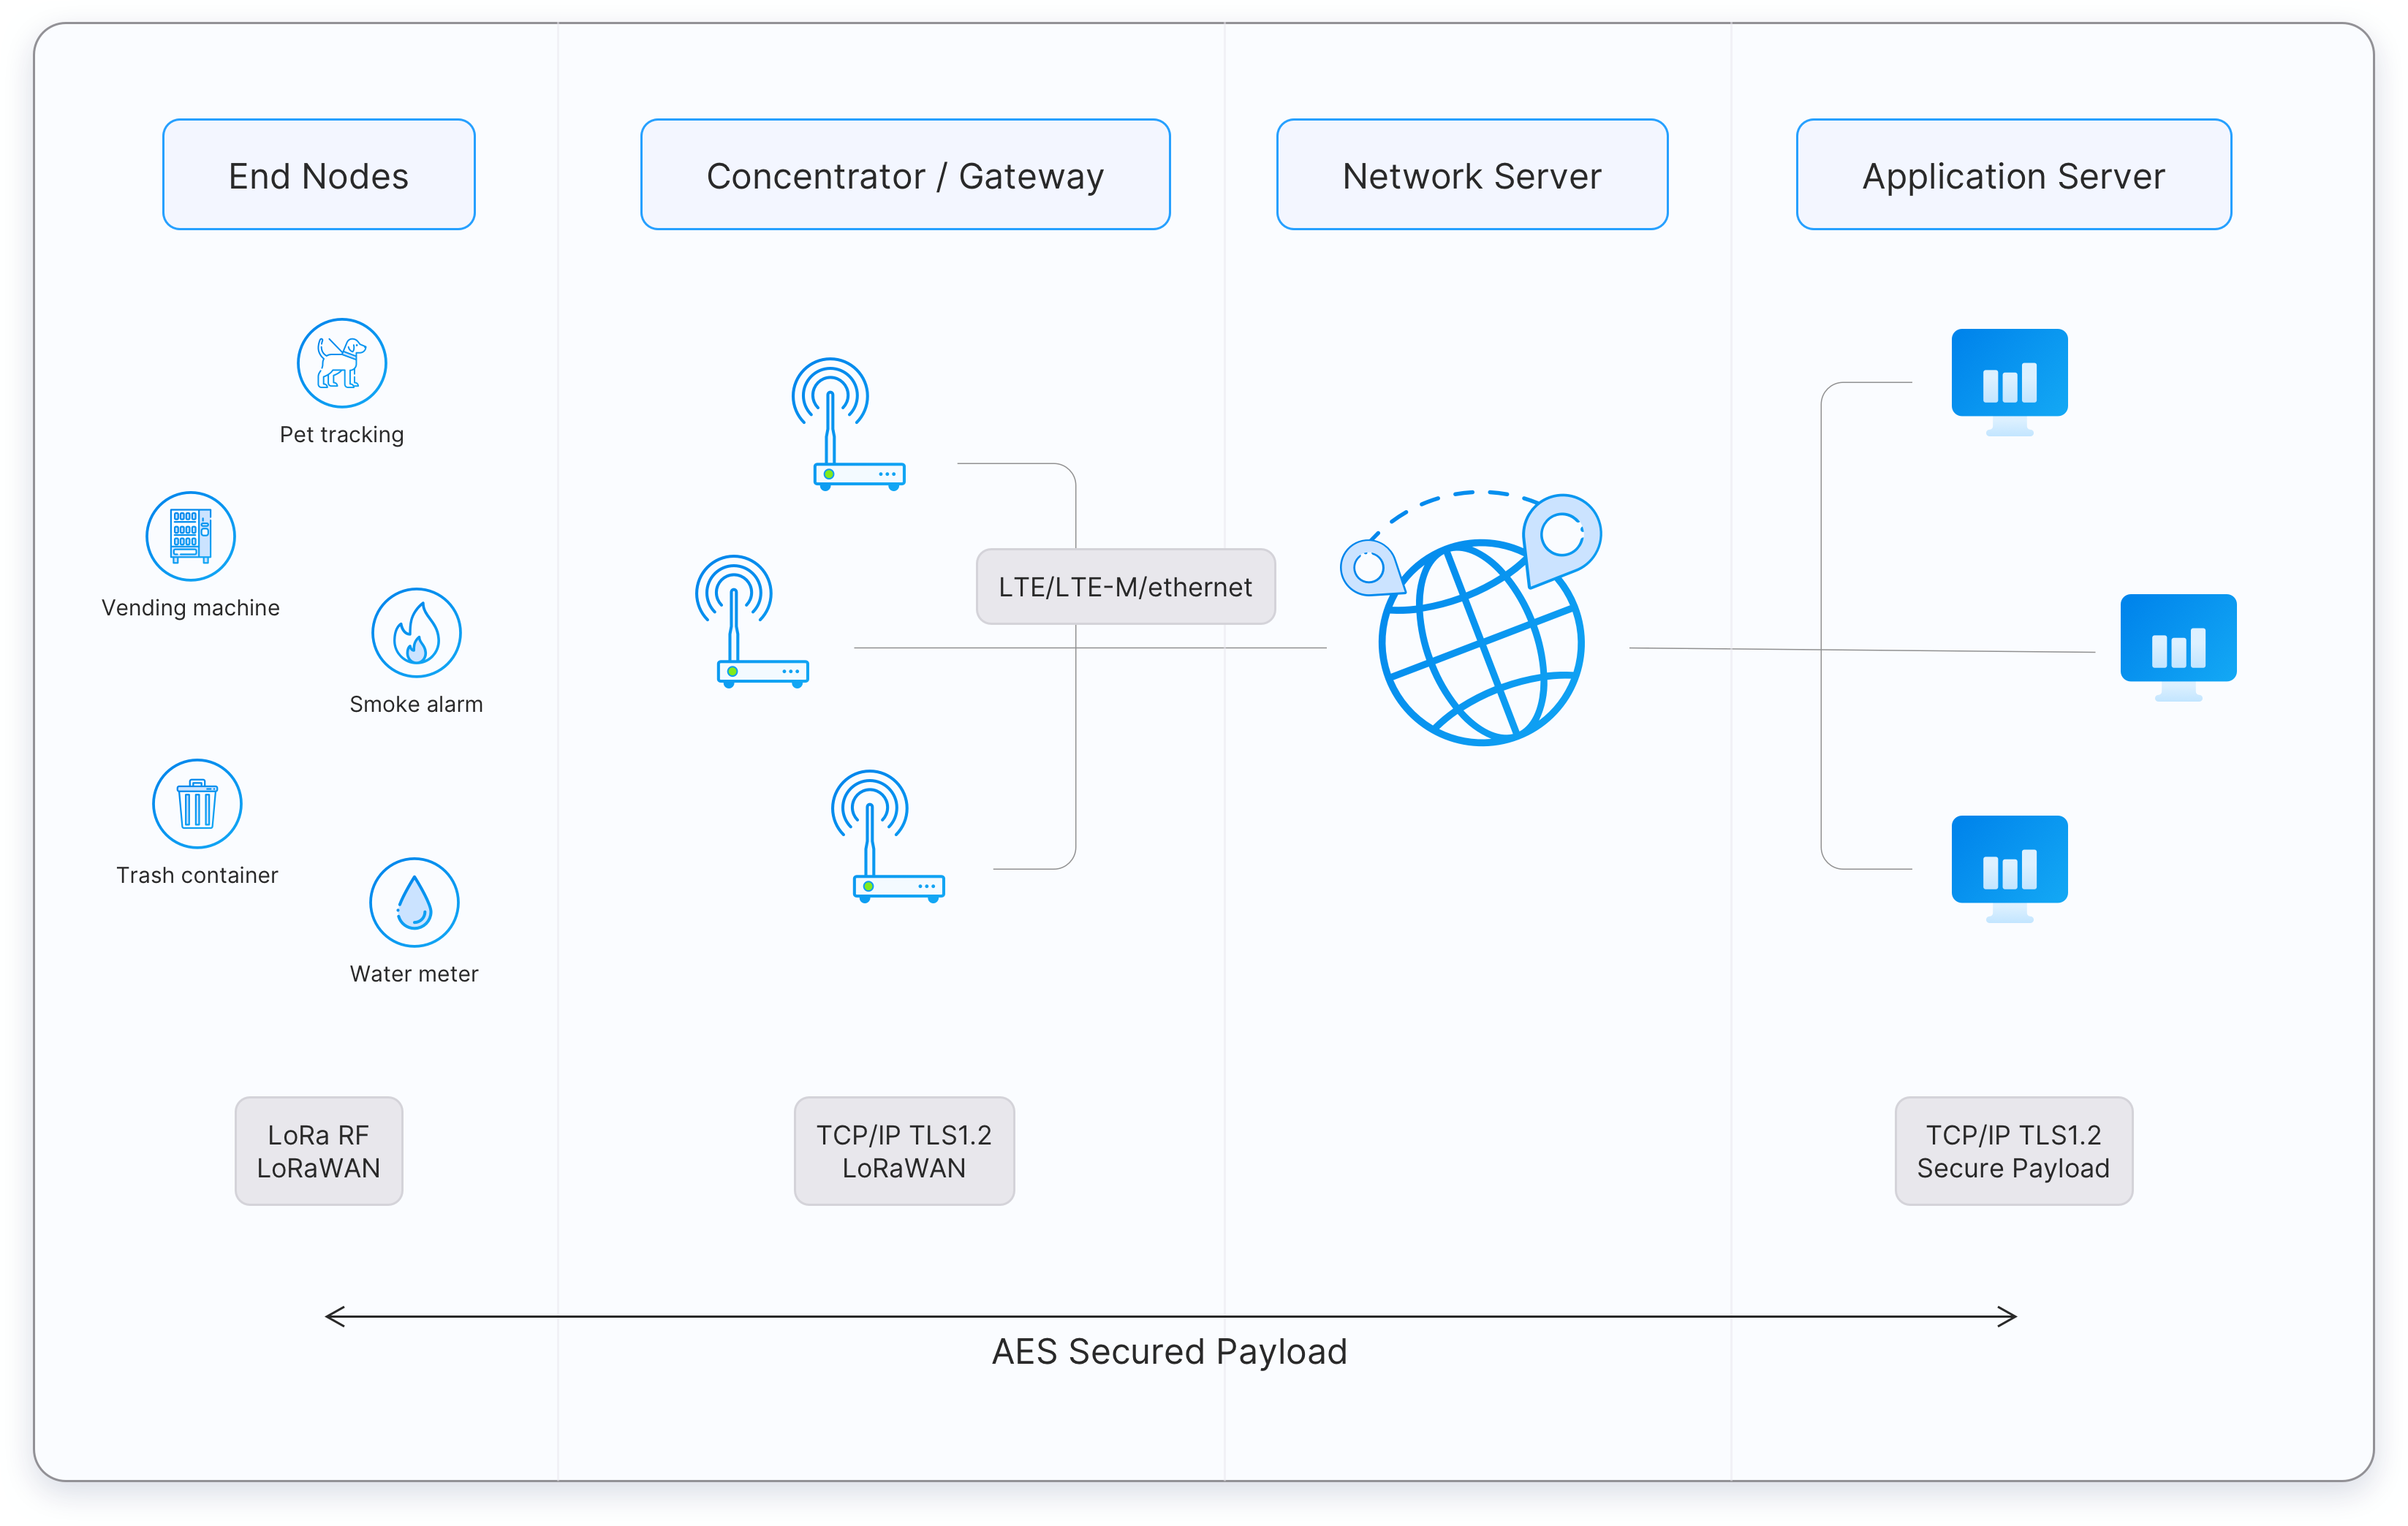
\includegraphics[width=0.8\textwidth]{figures/architecture_ttn.png}
    \caption{Arsitektur Jaringan LoRaWAN}
    \label{fig:lora_architecture}
\end{figure}
Jaringan LoRaWAN diterapkan menggunakan topologi \emph{star-of-stars}.
Gambar~\ref{fig:lora_architecture} menunjukkan arsitektur tingkat tinggi dari jaringan LoRaWAN dan komponen utamanya.
Penyebaran LoRaWAN khas terdiri dari elemen fungsional berikut:
\begin{enumerate}
    \item \textbf{End Devices}: Sensor atau aktuator yang mengirim atau menerima pesan nirkabel LoRa-modulated melalui gateway.
    \item \textbf{Gateways}: Penerima radio multi-saluran yang meneruskan pesan antara end devices dan Network Server.
    \item \textbf{Network Server}: Perangkat lunak terpusat yang bertanggung jawab atas operasi tingkat jaringan.
    \item \textbf{Application Servers}: Komponen perangkat lunak yang memproses data spesifik aplikasi secara aman.
    \item \textbf{Join Server}: Entitas khusus yang menangani aktivasi perangkat aman dan turunan kunci (tidak selalu digambarkan dalam diagram tingkat tinggi).
\end{enumerate}
End devices berkomunikasi dengan semua gateway dalam jangkauan radio. Gateway, pada gilirannya, terhubung ke Network Server melalui tautan backhaul (misalnya, Ethernet, seluler, atau Wi-Fi). Mekanisme akses medium didasarkan pada protokol tipe ALOHA; oleh karena itu, end devices tidak membuat asosiasi persisten dengan gateway tertentu. Pesan uplink dapat diterima oleh beberapa gateway secara bersamaan. Network Server melakukan \emph{deduplikasi pesan} dengan menyimpan hanya satu instance dari setiap pesan unik dan membuang salinan berlebih.
\subsection{End Devices}
\begin{figure}
    \centering
    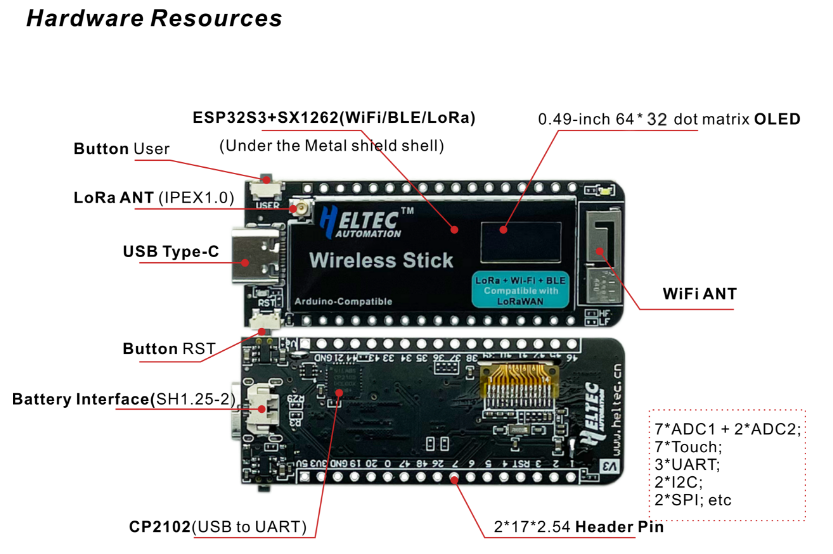
\includegraphics[width=0.6\textwidth]{figures/stick_v3.png}
    \caption{End Device LoRaWAN Heltec stick V3}
    \label{fig:lora_end_device}
\end{figure}
End device LoRaWAN biasanya merupakan sensor daya rendah, aktuator, atau kombinasi keduanya, sering kali dioperasikan dengan baterai yang memiliki masa pakai mulai dari beberapa bulan hingga lebih dari satu dekade. Perangkat ini berinteraksi dengan jaringan secara eksklusif melalui komunikasi RF berbasis LoRa. Modalitas penginderaan umum meliputi suhu, kelembaban, gerakan, dan parameter lingkungan. End devices beroperasi di bawah batasan peraturan yang ketat mengenai daya transmisi, duty cycle, dan penggunaan saluran, yang bersifat spesifik wilayah dan diberlakukan oleh spesifikasi parameter regional LoRaWAN.
Gambar~\ref{fig:lora_end_device} menunjukkan contoh end device LoRaWAN.
\subsection{Gateways}
\begin{figure}
    \centering
    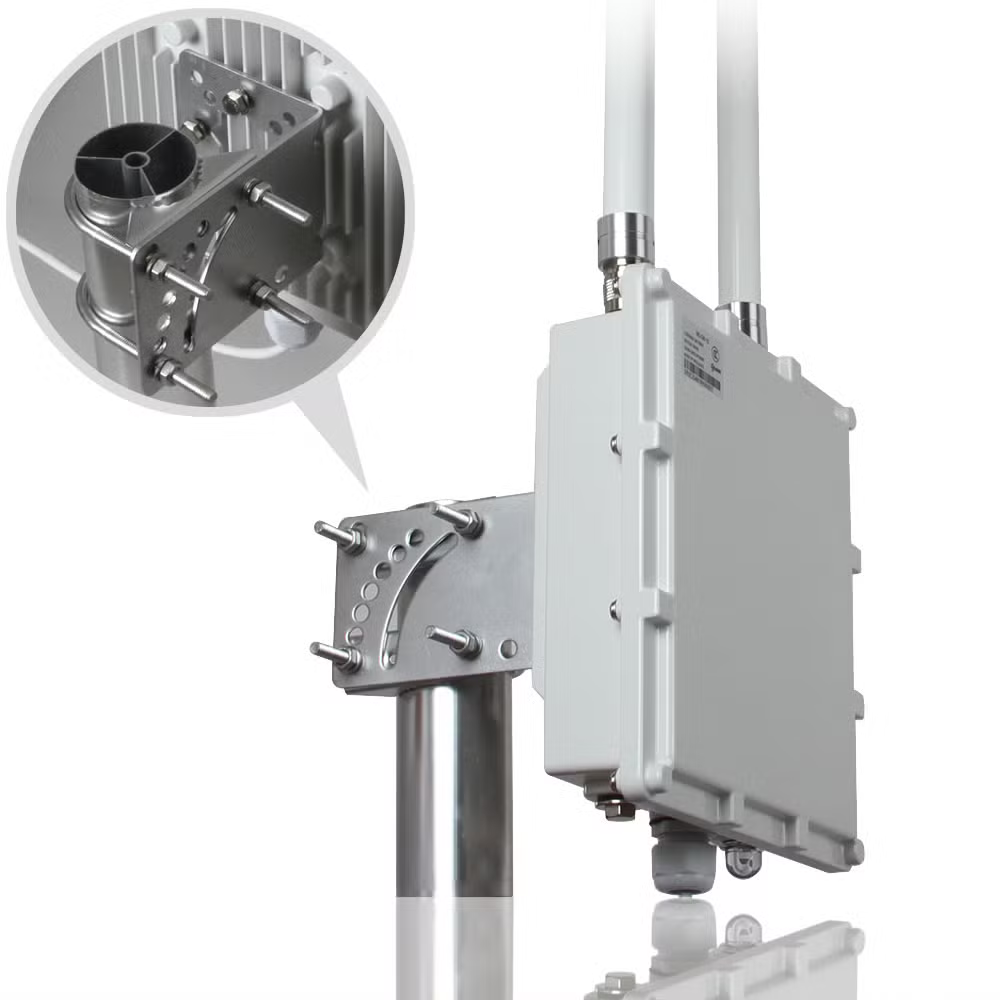
\includegraphics[width=0.6\textwidth]{figures/Ethernet-4G-Lorawan-Outdoor-Gateway-for-Remote-Street-Light-Management.png}
    \caption{Gateway LoRaWAN}
    \label{fig:lora_gateway}
\end{figure}
Gateway berfungsi sebagai jembatan transparan antara lapisan RF dan jaringan inti berbasis IP. Setiap gateway dikonfigurasi sebelumnya untuk berkomunikasi dengan Network Server yang ditentukan. Setelah menerima frame LoRa-modulated, gateway memberi stempel waktu, mengenkapsulasi dalam protokol standar (misalnya, LoRaWAN Backend Interfaces atau Semtech UDP Packet Forwarder), dan meneruskannya melalui backhaul ke Network Server.
Gambar~\ref{fig:lora_gateway} menunjukkan contoh gateway LoRaWAN.
Gateway LoRaWAN secara luas diklasifikasikan ke dalam dua kategori:
\begin{enumerate}
    \item \textbf{Gateway Indoor (Picocell)}:
          \begin{enumerate}
              \item Dirancang untuk penyebaran di lingkungan indoor residensial, komersial, atau industri.
              \item Biasanya memiliki antena terintegrasi atau antena eksternal pendek (misalnya, konektor pigtail).
              \item Hemat biaya dan cocok untuk cakupan di skenario indoor yang dalam seperti ruang bawah tanah atau bangunan bertingkat.
              \item Meskipun bentuknya kecil, beberapa gateway indoor dapat menerima sinyal dari perangkat yang berjarak beberapa kilometer di bawah kondisi propagasi yang menguntungkan.
          \end{enumerate}
    \item \textbf{Gateway Outdoor (Macrocell)}:
          \begin{enumerate}
              \item Dirancang untuk cakupan area luas di lingkungan perkotaan dan pedesaan.
              \item Sering dipasang pada struktur tinggi seperti menara seluler, atap gedung, atau tiang.
              \item Dilengkapi antena eksternal gain tinggi (misalnya, antena omnidirectional fiberglass) yang dihubungkan melalui kabel koaksial.
              \item Menunjukkan sensitivitas penerima yang lebih unggul dibandingkan rekan indoor.
              \item Dapat mendukung opsi konektivitas tambahan (misalnya, 3G/4G, GPS) untuk sinkronisasi dan redundansi backhaul.
              \item Dengan kandang lingkungan yang sesuai dan modifikasi antena, gateway indoor tertentu dapat digunakan kembali untuk penggunaan outdoor.
          \end{enumerate}
\end{enumerate}
\subsection{Network Server}
Network Server (NS) adalah komponen orkestrasi inti dari infrastruktur LoRaWAN. NS mengelola status jaringan, menegakkan kepatuhan protokol, dan memastikan routing data yang aman dan efisien. Tanggung jawab utama meliputi:
\begin{enumerate}
    \item Membangun keamanan end-to-end melalui enkripsi AES 128-bit menggunakan kunci sesi (NwkSKey untuk lapisan jaringan, AppSKey untuk lapisan aplikasi).
    \item Memvalidasi keaslian end devices dan integritas pesan yang diterima.
    \item Melakukan deduplikasi pesan uplink yang diterima dari beberapa gateway.
    \item Memilih gateway optimal untuk transmisi downlink berdasarkan kualitas sinyal dan waktu.
    \item Menjalankan algoritma Adaptive Data Rate (ADR) untuk secara dinamis menyesuaikan laju data perangkat dan daya transmisi demi efisiensi jaringan.
    \item Memverifikasi alamat perangkat (DevAddr) dan mengelola sesi perangkat.
    \item Mengakui frame uplink yang dikonfirmasi sesuai dengan persyaratan lapisan MAC.
    \item Merutekan payload aplikasi ke Application Server yang sesuai.
    \item Meneruskan pesan Join-Request dan Join-Accept antara end devices dan Join Server.
    \item Memproses dan merespons semua perintah MAC yang didefinisikan dalam spesifikasi LoRaWAN.
\end{enumerate}
\subsection{Application Server}
Application Server (AS) bertanggung jawab atas penanganan logika lapisan aplikasi. AS menerima payload aplikasi yang didekripsi dari Network Server, menafsirkan data sesuai dengan kebutuhan spesifik domain, dan dapat memprakarsai komunikasi downlink dengan menghasilkan payload aplikasi. Payload ini dikirim kembali ke end device target melalui Network Server. Penyebaran LoRaWAN tunggal dapat meng-host beberapa Application Server, masing-masing melayani kasus penggunaan atau penyewa yang berbeda. Analitik lanjutan, termasuk teknik machine learning dan artificial intelligence, sering diterapkan pada data yang dikumpulkan untuk menghasilkan wawasan yang dapat ditindaklanjuti dan mendukung pengambilan keputusan.
\subsection{Join Server}
Join Server (JS) adalah komponen kritis keamanan yang diperkenalkan dalam LoRaWAN 1.1 dan juga didukung dalam LoRaWAN 1.0.4 untuk keamanan yang ditingkatkan. Fungsi utamanya adalah:
\begin{enumerate}
    \item Penyimpanan aman kunci root (misalnya, AppKey dalam LoRaWAN 1.0, atau AppKey dan NwkKey dalam LoRaWAN 1.1).
    \item Memproses pesan Join-Request yang diprakarsai oleh end devices selama Over-the-Air Activation (OTAA).
    \item Menurunkan kunci sesi (NwkSKey dan AppSKey) setelah otentikasi berhasil.
    \item Mendistribusikan NwkSKey ke Network Server dan AppSKey ke Application Server secara aman.
\end{enumerate}
Pemisahan manajemen kunci ini meningkatkan keamanan dengan memastikan bahwa tidak ada entitas tunggal yang memiliki kunci sesi jaringan dan aplikasi, sehingga menegakkan prinsip hak akses minimal (least privilege) dan memungkinkan penyebaran multi-penyewa yang aman.
\section{Parameter Regional}
LoRaWAN beroperasi dalam pita spektrum radio Industrial, Scientific, and Medical (ISM) tanpa lisensi yang tersedia secara global. Mirip dengan Wi-Fi di pita 2,4\,GHz dan 5\,GHz, LoRaWAN memungkinkan penyebaran tanpa memerlukan lisensi spektrum individu. Namun, karena penggunaan frekuensi yang lebih rendah—biasanya antara 433\,MHz dan 928\,MHz—transmisi LoRaWAN mencapai jangkauan yang lebih jauh tetapi tunduk pada batasan peraturan yang lebih ketat dan spesifik negara. Untuk mendamaikan interoperabilitas global dengan kepatuhan lokal, LoRa Alliance telah mendefinisikan \emph{Parameter Regional} yang distandardisasi yang menentukan konfigurasi lapisan fisik dan MAC spesifik wilayah.
Parameter Regional ini menetapkan dasar teknis umum untuk setiap domain peraturan tetapi tidak mendefinisikan secara lengkap semua detail operasional. Operator jaringan dapat menerapkan saluran atau kebijakan tambahan di luar spesifikasi, yang sering disebut sebagai parameter \emph{Other}. Di beberapa yurisdiksi, beberapa rencana frekuensi diperbolehkan; misalnya, di Belanda, kedua pita EU863–870 dan EU433 diizinkan untuk penggunaan LoRaWAN.
Parameter Regional mencakup:
\begin{enumerate}
    \item Spesifikasi lapisan fisik, termasuk:
          \begin{enumerate}
              \item Rencana frekuensi (saluran)
              \item Saluran wajib untuk join jaringan
              \item Laju data dan spreading factor yang diizinkan
              \item Batas daya transmisi (EIRP)
          \end{enumerate}
    \item Batasan lapisan MAC, seperti:
          \begin{enumerate}
              \item Ukuran payload maksimum per laju data
              \item Waktu dan frekuensi jendela penerimaan
              \item Batasan duty cycle dan dwell time (jika berlaku)
          \end{enumerate}
\end{enumerate}
Dokumen Parameter Regional resmi (RP002-1.0.4) mendefinisikan tiga belas rencana frekuensi berbeda, masing-masing diberi ID Rencana unik dan nama umum, sebagaimana dirangkum di bawah ini.
\subsection{Rencana Frekuensi}
\begin{enumerate}
    \item Plan ID 1: EU863–870 (nama umum: EU868)
    \item Plan ID 2: US902–928 (nama umum: US915)
    \item Plan ID 3: CN779–787 (nama umum: CN779)
    \item Plan ID 4: EU433 (nama umum: EU433)
    \item Plan ID 5: AU915–928 (nama umum: AU915)
    \item Plan ID 6: CN470–510 (nama umum: CN470)
    \item Plan ID 7: AS923-1 (nama umum: AS923)
    \item Plan ID 8: AS923-2 (nama umum: AS923-2)
    \item Plan ID 9: AS923-3 (nama umum: AS923-3)
    \item Plan ID 10: KR920–923 (nama umum: KR920)
    \item Plan ID 11: IN865–867 (nama umum: IN865)
    \item Plan ID 12: RU864–870 (nama umum: RU864)
    \item Plan ID 13: AS923-4 (nama umum: AS923-4)
\end{enumerate}
Setiap rencana sesuai dengan satu atau lebih negara, sebagaimana dirinci dalam Tabel Referensi Silang Negara LoRa Alliance. Meskipun pengetahuan komprehensif tentang semua rencana tidak diperlukan, pita EU863–870 dan US902–928 ditekankan dalam konteks sertifikasi karena adopsinya yang luas.
\subsection{Pengaturan Default untuk Semua Wilayah}
Parameter waktu dan operasional tertentu direkomendasikan secara seragam di semua implementasi regional untuk memastikan interoperabilitas dasar. Nilai default ini adalah sebagai berikut:
\begin{enumerate}
    \item \textbf{RECEIVE\_DELAY1 (RX1 Delay)}: 1 detik
    \item \textbf{RECEIVE\_DELAY2 (RX2 Delay)}: 2 detik (didefinisikan sebagai RX1 Delay + 1 detik)
    \item \textbf{JOIN\_ACCEPT\_DELAY1}: 5 detik
    \item \textbf{JOIN\_ACCEPT\_DELAY2}: 6 detik
\end{enumerate}
Default ini dapat diganti melalui perintah MAC (misalnya, \texttt{RXTimingSetupReq}) atau selama provisioning perangkat, tetapi penyimpangan harus dikomunikasikan ke Network Server selama komisioning. Network Server dapat menolak konfigurasi waktu non-standar untuk menjaga integritas jaringan.
\subsection{Indonesia: Pita AS923-2}
\label{subsec:indonesia_as923}
Di Indonesia, operasi LoRaWAN diatur di bawah rencana frekuensi \textbf{AS923-2}, yang merupakan varian dari spesifikasi regional AS923 yang lebih luas yang didefinisikan dalam dokumen Parameter Regional LoRaWAN RP002-1.0.4. Rencana ini mengakomodasi sub-pita spesifik yang dialokasikan oleh otoritas peraturan Indonesia, yaitu pita ISM \textbf{920–923 MHz}.
Kerangka kerja regional AS923 menggunakan mekanisme offset frekuensi untuk mendukung beberapa implementasi nasional menggunakan spesifikasi dasar yang sama. Untuk Indonesia, rencana ini ditetapkan sebagai \textbf{AS923-2}, sesuai dengan offset frekuensi:
\begin{enumerate}
    \item \texttt{AS923\_FREQ\_OFFSET} = \texttt{0xFFFFB9B0} (bilangan bulat bertanda 32-bit)
    \item \texttt{AS923\_FREQ\_OFFSET\_HZ} = $-1.80$~MHz
\end{enumerate}
Offset ini menggeser saluran default nominal AS923 dari 923.2/923.4~MHz ke \textbf{921.4~MHz} dan \textbf{921.6~MHz}, yang merupakan saluran default wajib untuk semua end-device AS923-2 di Indonesia.
\begin{enumerate}
    \item \textbf{Saluran Default dan Join}:
          Setiap end-device harus mengimplementasikan dua saluran default berikut untuk operasi normal dan transmisi Join-Request:
    \item Uplink/Downlink: 921.4~MHz (DR2–DR5)
    \item Uplink/Downlink: 921.6~MHz (DR2–DR5)
          Saluran ini menggunakan modulasi LoRa dengan bandwidth 125~kHz. Laju data Join-Request dibatasi pada DR2–DR5 (SF10–SF7) untuk memastikan kompatibilitas dengan batasan dwell time 400~ms yang diberlakukan di banyak yurisdiksi AS923 hingga dikonfigurasi ulang oleh jaringan.
    \item \textbf{Pengkodean Laju Data dan TXPower}:
          Laju data yang didukung adalah:
    \item DR0–DR5 (minimum untuk sertifikasi)
    \item DR0–DR7 (dukungan opsional penuh, termasuk DR6: LoRa SF7/250~kHz dan DR7: FSK 50~kbps)
          EIRP maksimum adalah \textbf{+16 dBm}. Level TXPower didefinisikan relatif terhadap maksimum ini dalam langkah 2~dB (TXPower 0 = +16 dBm, TXPower 1 = +14 dBm, dll.).
    \item \textbf{Dwell Time dan Kepatuhan Peraturan}:
          Perangkat AS923-2 di Indonesia harus mendukung perintah MAC \texttt{TxParamSetupReq} untuk menerima konfigurasi dwell time dari Network Server. Secara default, perangkat mengasumsikan \texttt{UplinkDwellTime} = 1 (batas 400~ms) hingga dikonfigurasi ulang secara eksplisit. Dwell time downlink selalu diatur ke 0 (tanpa batasan).
    \item \textbf{Jendela Penerimaan}:
    \item RX1 menggunakan saluran yang sama dengan uplink. Laju data downlink ditentukan oleh DR uplink dan RX1DROffset (0–7).
    \item RX2 menggunakan frekuensi tetap \textbf{921.4~MHz} (yaitu, 923.2~MHz + \texttt{AS923\_FREQ\_OFFSET\_HZ}) dengan DR2 (SF10, 125~kHz).
    \item \textbf{Fleksibilitas Rencana Saluran}:
          Meskipun hanya dua saluran default yang diwajibkan, end-device harus mendukung struktur data saluran untuk setidaknya 24 saluran. Saluran tambahan dapat dikonfigurasi melalui CFList dalam pesan Join-Accept atau melalui perintah MAC (misalnya, \texttt{NewChannelReq}, \texttt{LinkADRReq}).
    \item \textbf{Listen-Before-Talk (LBT)}:
          Meskipun tidak secara eksplisit diwajibkan untuk Indonesia dalam RP002-1.0.4, perangkat AS923 yang beroperasi di wilayah dengan persyaratan LBT (misalnya, Jepang) harus mematuhi ARIB STD-T108. Produsen perangkat yang menargetkan Indonesia harus memverifikasi peraturan lokal saat ini, karena kebijakan manajemen spektrum dapat berkembang.
\end{enumerate}
Secara ringkas, penyebaran LoRaWAN di Indonesia harus mematuhi profil AS923-2, yang memastikan kepatuhan peraturan sekaligus mempertahankan interoperabilitas dalam ekosistem AS923 yang lebih luas. Operator jaringan dan vendor perangkat harus mengonfigurasi offset frekuensi dan parameter dwell time secara tepat selama komisioning untuk menjamin operasi yang benar.
\section{Relay LoRaWAN}
\begin{figure}
    \centering
    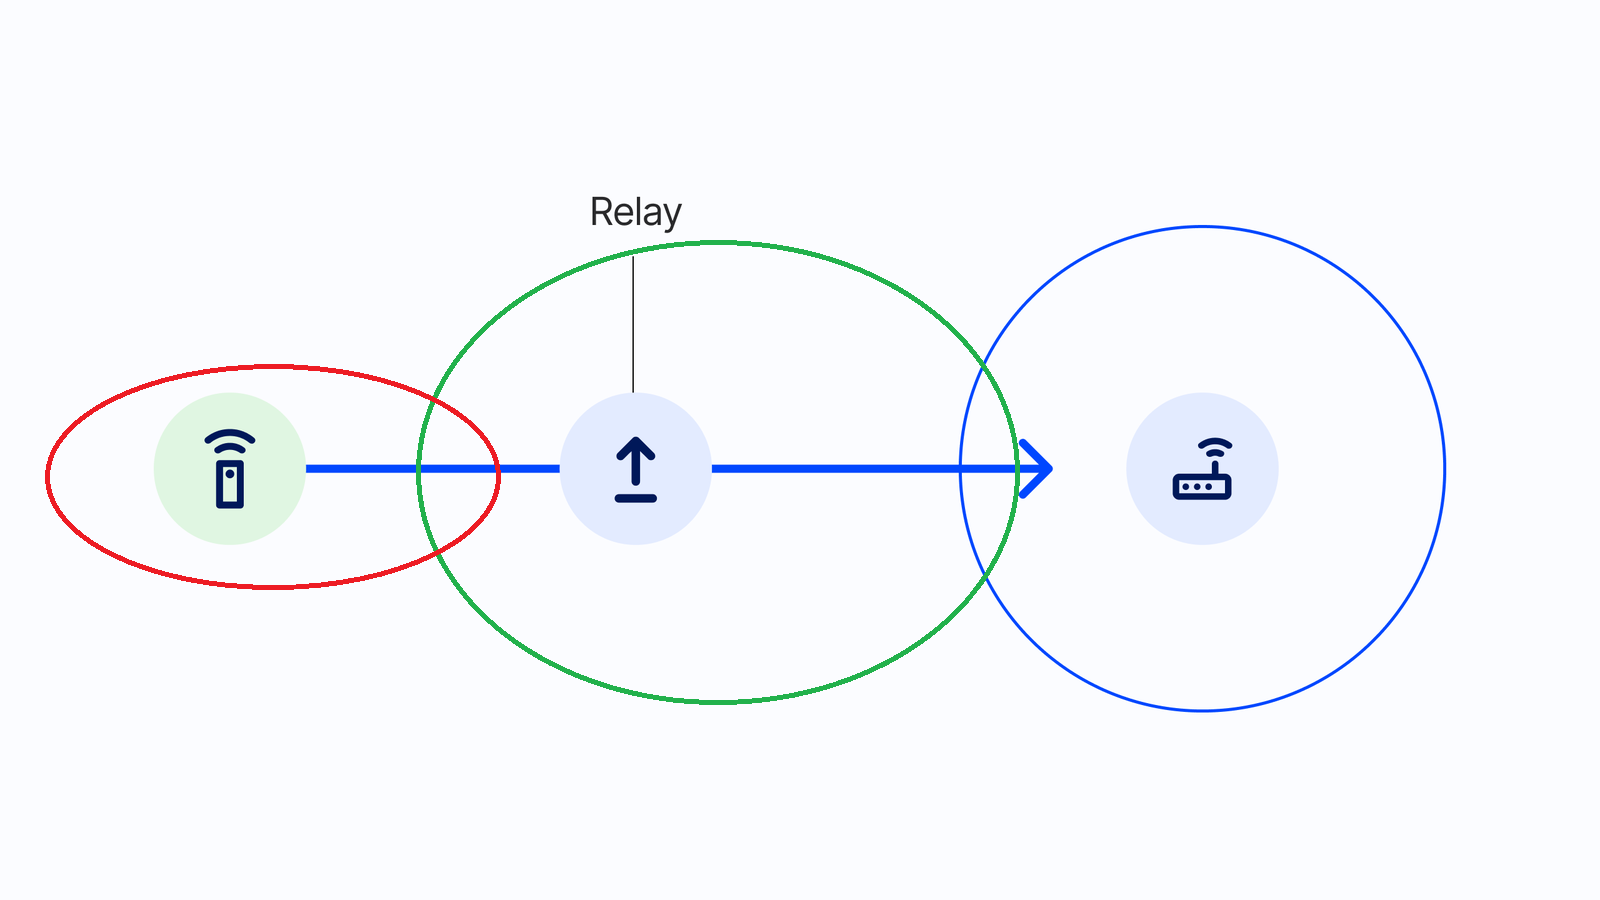
\includegraphics[width=0.8\textwidth]{figures/relay-placement.png}
    \caption{Arsitektur Relay LoRaWAN}
    \label{fig:lora_relay}
\end{figure}
Relay LoRaWAN menyediakan solusi hemat biaya untuk memperluas cakupan jaringan dalam skenario di mana komunikasi langsung antara end devices dan gateway terganggu karena jarak yang berlebihan, hambatan fisik, atau redaman sinyal. Relay beroperasi sebagai perantara berdaya rendah dan berbiaya rendah yang meneruskan pesan antara end devices dan infrastruktur LoRaWAN. Dari perspektif Network Server, relay secara fungsional tidak dapat dibedakan dari end device standar.
Gambar~\ref{fig:lora_relay} menggambarkan arsitektur sistem relay LoRaWAN.
\subsection{Strategi Penempatan Relay}
Penyebaran relay secara ekonomis dibenarkan ketika hanya sejumlah kecil end devices yang mengalami masalah konektivitas. Sebaliknya, jika kekurangan cakupan memengaruhi sebagian besar jaringan, pemasangan gateway tambahan biasanya lebih tepat.
\subsection{Persyaratan Relay}
Persyaratan fungsional dan teknis untuk relay LoRaWAN secara formal didefinisikan dalam \emph{Spesifikasi Relay LoRaWAN\textsuperscript{\textregistered}} (TS011-1.0.0). Prasyarat implementasi utama meliputi:
\begin{enumerate}
    \item End device harus mengimplementasikan:
          \begin{enumerate}
              \item Spesifikasi Lapisan MAC LoRaWAN (TS001) versi 1.0.4.
              \item Spesifikasi Parameter Regional RP2-1.0.3.
              \item Firmware LoRa Basics Modem (rilis eksperimental tersedia dari Semtech).
          \end{enumerate}
    \item Perangkat keras end device harus menggabungkan salah satu transceiver LoRa sub-GHz berikut:
          \begin{enumerate}
              \item SX1261/2
              \item LR1110
              \item LR1120
              \item LR1121
          \end{enumerate}
    \item LoRaWAN Network Server (misalnya, The Things Stack) harus mendukung spesifikasi relay.
    \item Gateway tidak memerlukan modifikasi atau pembaruan firmware untuk mendukung fungsionalitas relay.
\end{enumerate}
\subsection{Operasi Relay}
Komunikasi antara end device dan Network Server melalui relay mengikuti urutan terstruktur:
\begin{enumerate}
    \item Sebelum komunikasi, end device dan relay dikonfigurasi sebelumnya dengan parameter saluran bersama (frekuensi, laju data) untuk tautan langsung mereka.
    \item Untuk memulai komunikasi, end device mengirimkan frame \emph{Wake-on-Radio} (WOR). Frame ini memiliki dua tujuan:
          \begin{enumerate}
              \item Membangunkan relay dari mode tidur.
              \item Menyampaikan parameter radio (frekuensi dan laju data) untuk transmisi uplink berikutnya.
          \end{enumerate}
    \item Dua jenis frame WOR didefinisikan, dapat dibedakan berdasarkan konten payload:
          \begin{enumerate}
              \item Relay Join-Request
              \item Relay Uplink (uplink Kelas A)
          \end{enumerate}
    \item Relay beroperasi dalam keadaan tidur berdaya rendah dan secara berkala melakukan \emph{Channel Activity Detection} (CAD) untuk memantau frame WOR masuk. Parameter waktu utama meliputi:
          \begin{enumerate}
              \item Durasi CAD: 25 ms hingga 1 s (tergantung konfigurasi default).
              \item Periodisitas CAD: interval antara operasi CAD berturut-turut.
              \item Panjang preamble WOR: hingga 1 s, memastikan probabilitas deteksi tinggi selama jendela CAD singkat.
          \end{enumerate}
    \item Setelah mendeteksi aktivitas LoRa selama CAD, relay beralih ke mode penerima setelah penundaan \emph{CadToRx}. Jika frame WOR yang didemodulasi valid, relay merespons dengan frame \emph{WOR-ACK} yang berisi:
          \begin{enumerate}
              \item \texttt{CadToRx}: penundaan dari deteksi CAD ke kesiapan penerimaan.
              \item \texttt{Forward}: status kemampuan penerusan relay.
              \item \texttt{RelayDataRate}: laju data untuk penerusan upstream ke Network Server.
              \item \texttt{XTALAccuracy}: akurasi osilator kristal relay.
              \item \texttt{CADPeriodicity}: interval antara pemindaian CAD.
              \item \texttt{TOffset}: waktu antara awal CAD dan akhir penerimaan preamble WOR.
          \end{enumerate}
    \item End device menggunakan parameter WOR-ACK untuk menyinkronkan transmisi berikutnya dengan relay.
    \item End device kemudian mengirimkan frame uplink LoRaWAN-nya. Relay menerima frame ini, menambahkan header metadata 6-byte, dan mengenkapsulasi hasilnya sebagai \emph{Relay Uplink FRMPayload}. Payload ini dikirim ke Network Server menggunakan FPort 226.
    \item Pesan downlink dari Network Server (FPort 226) diterima oleh relay di jendela RX1 atau RX2. Relay mengekstrak payload asli dan meneruskannya ke end device selama jendela \emph{Relay Receive} (RXR) yang didedikasikan.
\end{enumerate}
\subsection{Parameter Regional untuk Relay}
Parameter lapisan fisik khusus relay didefinisikan per pita regional. Contohnya meliputi:
\begin{enumerate}
    \item \textbf{EU868 (EU863–870 MHz)}:
          \begin{enumerate}
              \item Saluran WOR (end device $\rightarrow$ relay):
                    \begin{enumerate}
                        \item Saluran 0: 856.1 MHz
                        \item Saluran 1: 865.5 MHz
                    \end{enumerate}
              \item Saluran WOR-ACK (relay $\rightarrow$ end device):
                    \begin{enumerate}
                        \item Saluran 0: 865.3 MHz
                        \item Saluran 1: 865.9 MHz
                    \end{enumerate}
              \item Bandwidth: 125 kHz
              \item Spreading Factor: SF9
          \end{enumerate}
    \item \textbf{US915 (US902–928 MHz)}:
          \begin{enumerate}
              \item Saluran WOR (end device $\rightarrow$ relay):
                    \begin{enumerate}
                        \item Saluran 0: 916.7 MHz
                        \item Saluran 1: 919.9 MHz
                    \end{enumerate}
              \item Saluran WOR-ACK (relay $\rightarrow$ end device):
                    \begin{enumerate}
                        \item Saluran 0: 918.3 MHz
                        \item Saluran 1: 918.3 MHz
                    \end{enumerate}
              \item Bandwidth: 500 kHz
              \item Spreading Factor: SF10
          \end{enumerate}
    \item Untuk wilayah lain (AU915, CN470, AS923, KR920, IN865, RU864), frekuensi saluran relay, bandwidth, dan spreading factor ditentukan dalam dokumen Parameter Regional LoRaWAN RP002-1.0.4.
\end{enumerate}
\subsection{Model Keamanan}
Komunikasi relay menggunakan kerangka kerja keamanan khusus untuk memastikan integritas dan kerahasiaan frame WOR dan WOR-ACK:
\begin{enumerate}
    \item Kunci sesi standar (\texttt{AppSKey}, \texttt{NwkSKey}) tidak cukup untuk mengamankan frame kontrol relay.
    \item Kunci root baru, \emph{Root Relay Session Key} (\texttt{RootWorSKey}), diturunkan oleh end device:
          \begin{enumerate}
              \item Dari \texttt{NwkSKey} dalam LoRaWAN 1.0.x.
              \item Dari \texttt{NwkSEncKey} dalam LoRaWAN 1.1.x dan seterusnya.
          \end{enumerate}
    \item Network Server menyediakan \texttt{RootWorSKey} yang sama ke relay selama komisioning.
    \item End device dan relay secara independen menurunkan dua kunci sesi dari \texttt{RootWorSKey} dan \texttt{DevAddr}:
          \begin{enumerate}
              \item \texttt{WorSIntKey}: digunakan untuk menghitung dan memverifikasi Message Integrity Code (MIC) frame WOR dan WOR-ACK.
              \item \texttt{WorSEncKey}: digunakan untuk mengenkripsi dan mendekripsi payload frame WOR dan WOR-ACK.
          \end{enumerate}
\end{enumerate}
\section{Jenis Pesan}
LoRaWAN mendefinisikan serangkaian jenis pesan terstruktur untuk memfasilitasi komunikasi aman dan efisien antara end devices, gateway, dan entitas jaringan. Pesan-pesan ini mengangkut perintah Medium Access Control (MAC) dan data lapisan aplikasi. Memahami klasifikasi pesan, struktur, enkripsi, dan mekanisme integritas sangat penting untuk interoperabilitas dan kepatuhan keamanan, terutama dalam versi LoRaWAN 1.0.x dan 1.1.
\subsection{Pesan Uplink dan Downlink}
Pesan dalam LoRaWAN dikategorikan berdasarkan arah transmisinya:
\begin{enumerate}
    \item \textbf{Pesan uplink}: Berasal dari end devices dan diteruskan ke Network Server melalui satu atau lebih gateway. Bergantung pada tujuannya, Network Server meneruskan pesan ini ke Application Server atau Join Server.
    \item \textbf{Pesan downlink}: Dikirim oleh Network Server ke end device tertentu dan dikirim melalui gateway yang dipilih. Pesan ini dapat berasal dari Network Server itu sendiri, Application Server, atau Join Server.
\end{enumerate}
\subsection{Jenis Pesan MAC}
LoRaWAN menentukan jenis pesan MAC yang berbeda untuk kontrol jaringan dan transportasi data. Enumerasi berikut menguraikan jenis pesan yang didukung dalam LoRaWAN 1.0.x dan 1.1:
\begin{enumerate}
    \item \textbf{Join-request}: Pesan uplink yang digunakan selama Over-the-Air Activation (OTAA) untuk memulai sesi.
    \item \textbf{Join-accept}: Respons downlink terhadap Join-request, menyediakan parameter sesi.
    \item \textbf{Unconfirmed Data Up}: Frame data uplink yang tidak memerlukan acknowledgment.
    \item \textbf{Unconfirmed Data Down}: Frame data downlink yang tidak memerlukan acknowledgment.
    \item \textbf{Confirmed Data Up}: Frame data uplink yang memerlukan acknowledgment dari penerima.
    \item \textbf{Confirmed Data Down}: Frame data downlink yang memerlukan acknowledgment dari end device.
    \item \textbf{Rejoin-request} (hanya LoRaWAN 1.1): Pesan uplink yang digunakan untuk membuat ulang konteks sesi tanpa reaktivasi penuh; mendukung tiga subtipe (0, 1, 2).
    \item \textbf{Proprietary}: Dicadangkan untuk ekstensi khusus vendor.
    \item \textbf{RFU} (LoRaWAN 1.0.x): Dicadangkan untuk penggunaan di masa depan; digunakan kembali sebagai Rejoin-request dalam 1.1.
\end{enumerate}
\subsection{Pesan Join-Request, Rejoin-Request, dan Join-Accept}
\begin{enumerate}
    \item \textbf{Join-request}:
          \begin{enumerate}
              \item Diprakarsai oleh end device.
              \item Dalam LoRaWAN 1.0.4 dan sebelumnya, diteruskan oleh Network Server ke Application Server.
              \item Dalam LoRaWAN 1.1 dan 1.0.4+, diteruskan ke Join Server.
              \item Dikirim tanpa enkripsi.
          \end{enumerate}
    \item \textbf{Join-accept}:
          \begin{enumerate}
              \item Dihasilkan oleh Join Server (1.1 dan 1.0.4+) atau Application Server (sebelum 1.0.4).
              \item Dirutekan ke end device melalui Network Server.
              \item Kunci enkripsi tergantung pada versi LoRaWAN dan pesan pemicu:
                    \begin{enumerate}
                        \item LoRaWAN 1.0: dienkripsi dengan \texttt{AppKey}.
                        \item LoRaWAN 1.1:
                        \item Dipicu oleh Join-request: dienkripsi dengan \texttt{NwkKey}.
                        \item Dipicu oleh Rejoin-request (Tipe 0, 1, 2): dienkripsi dengan \texttt{JSEncKey}.
                    \end{enumerate}
          \end{enumerate}
    \item \textbf{Rejoin-request} (hanya LoRaWAN 1.1):
          \begin{enumerate}
              \item Diprakarsai oleh end device untuk menyegarkan kunci sesi atau bergabung kembali setelah roaming.
              \item Tiga tipe didefinisikan (0, 1, 2), berbeda dalam cakupan pengenal (NetID vs. JoinEUI).
              \item Selalu direspons dengan pesan Join-accept.
          \end{enumerate}
\end{enumerate}
\subsection{Pesan Data}
\begin{figure}
    \centering
    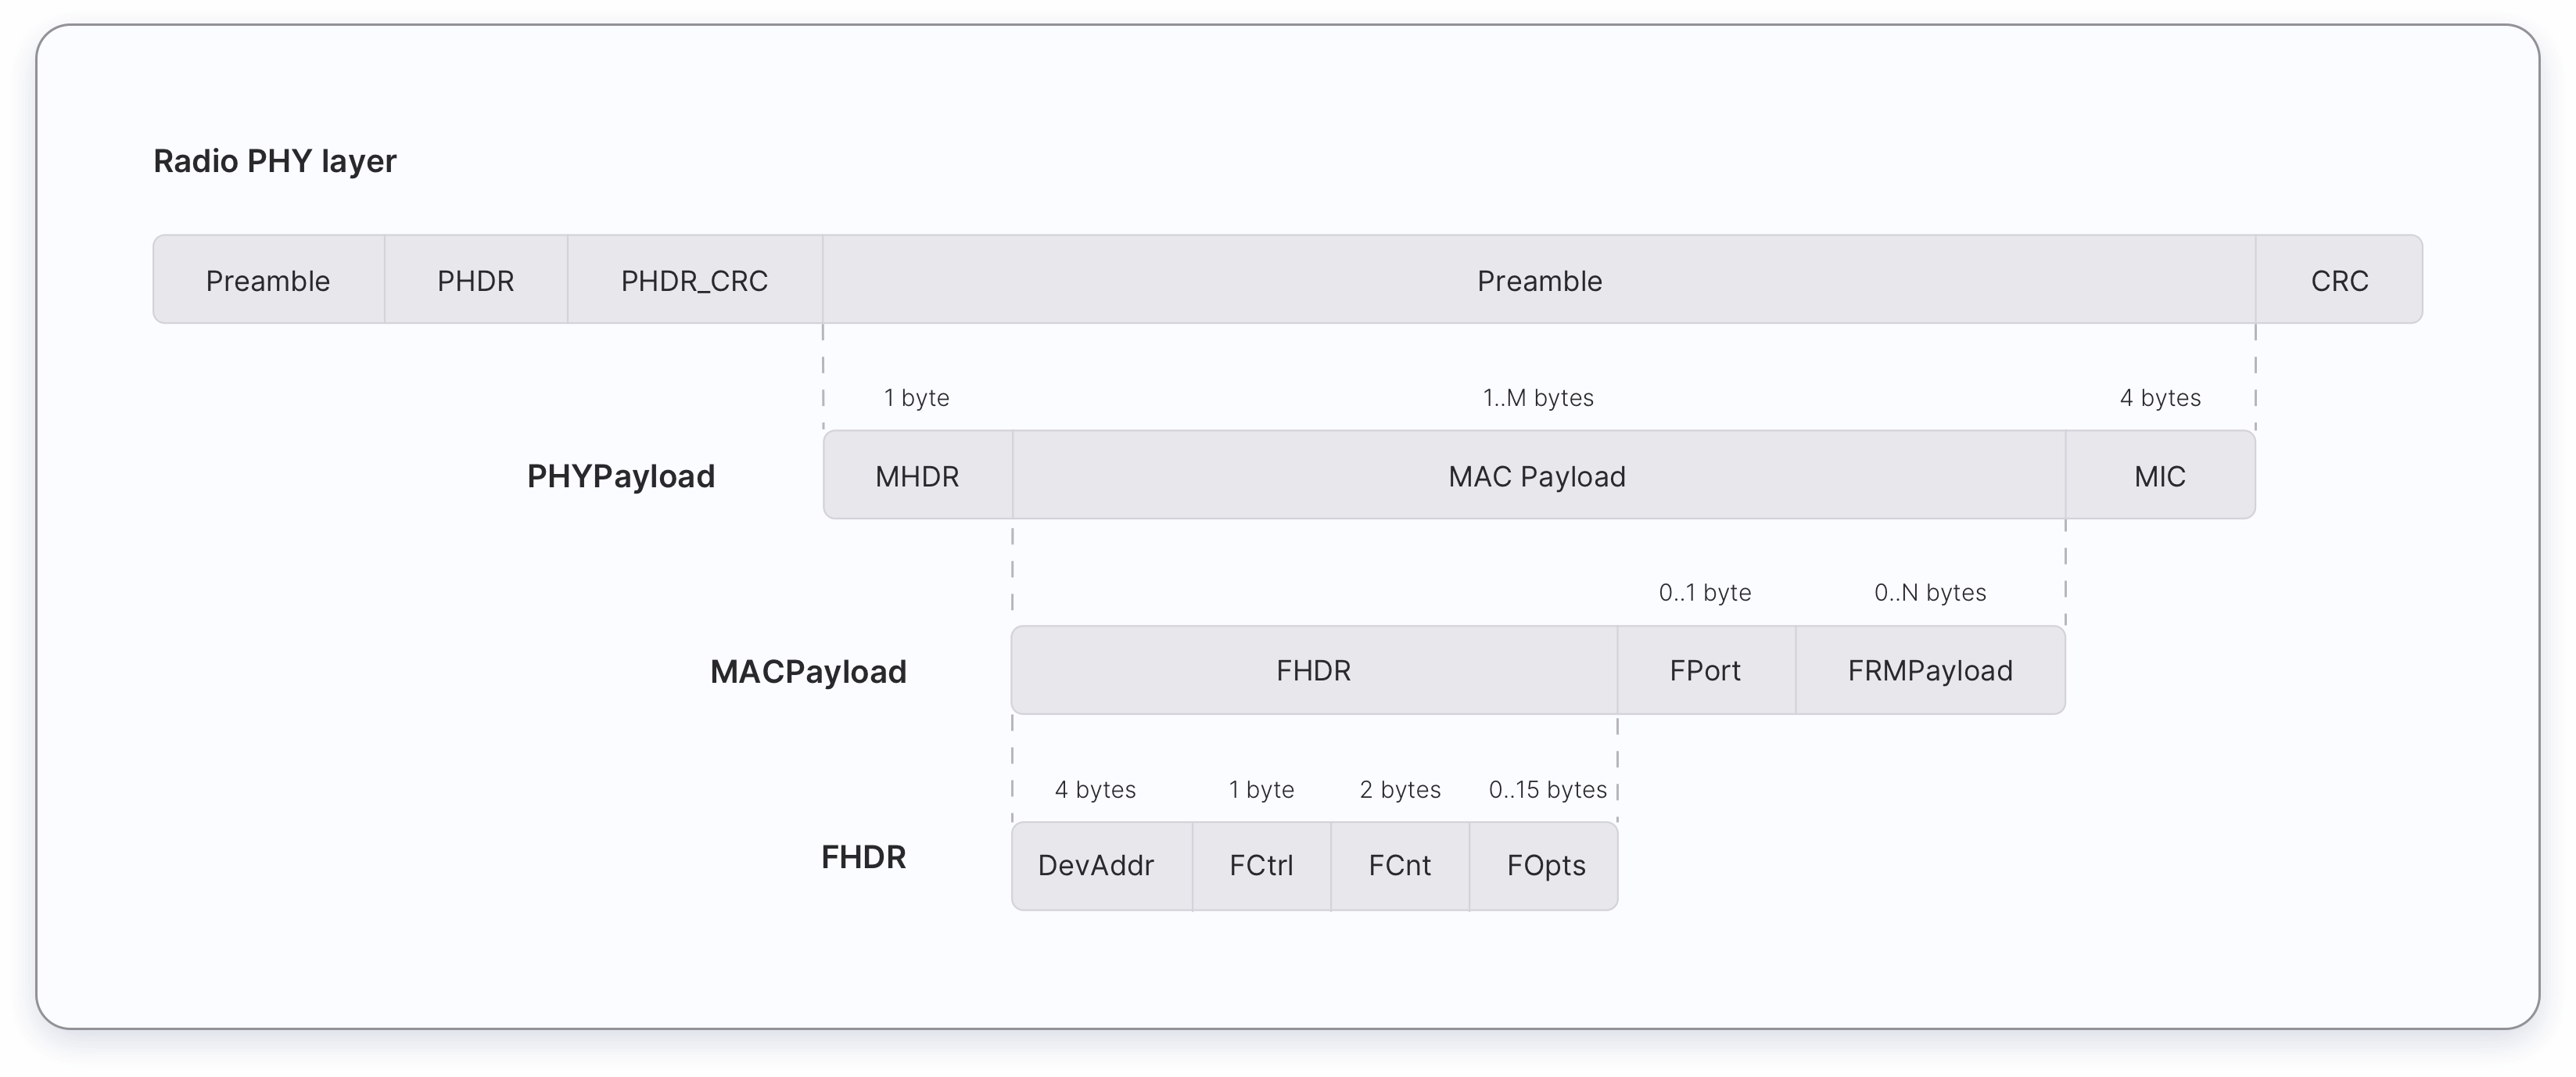
\includegraphics[width=0.8\textwidth]{figures/payload.png}
    \caption{Struktur Pesan Data LoRaWAN}
    \label{fig:lora_data_message}
\end{figure}
Pesan data mengangkut payload aplikasi dan/atau perintah MAC. Empat tipe ada, konsisten di seluruh LoRaWAN 1.0.x dan 1.1:
Gambar~\ref{fig:lora_data_message} menggambarkan struktur pesan data LoRaWAN.
\begin{enumerate}
    \item Unconfirmed Data Up
    \item Unconfirmed Data Down
    \item Confirmed Data Up
    \item Confirmed Data Down
\end{enumerate}
Pesan data terdiri dari payload MAC yang disusun sebagai berikut:
\begin{enumerate}
    \item \textbf{Frame Header (FHDR)}: 7–22 byte, berisi:
          \begin{enumerate}
              \item \texttt{DevAddr} (4 byte)
              \item \texttt{FCtrl} (1 byte)
              \item \texttt{FCnt} (2 byte)
              \item \texttt{FOpts} (0–15 byte)
          \end{enumerate}
    \item \textbf{FPort} (0–1 byte, opsional): Menunjukkan konten FRMPayload.
    \item \textbf{FRMPayload} (0–N byte, opsional): Mengangkut perintah MAC atau data aplikasi.
\end{enumerate}
Panjang payload MAC maksimum tergantung pada wilayah dan laju data, sebagaimana didefinisikan dalam spesifikasi Parameter Regional.
\subsection{Mengirim Perintah MAC dan Data Spesifik Aplikasi}
Perintah MAC dan data aplikasi saling eksklusif dalam field FRMPayload tetapi dapat berdampingan dalam pesan jika perintah MAC ditempatkan di FOpts dan data aplikasi di FRMPayload.
\begin{enumerate}
    \item \textbf{Perintah MAC di FOpts}:
          \begin{enumerate}
              \item Panjang total tidak boleh melebihi 15 byte.
              \item Dalam LoRaWAN 1.0.x: dikirim tanpa enkripsi.
              \item Dalam LoRaWAN 1.1: dienkripsi menggunakan \texttt{NwkSEncKey}.
          \end{enumerate}
    \item \textbf{Perintah MAC atau data aplikasi di FRMPayload}:
          \begin{enumerate}
              \item Memerlukan keberadaan field FPort.
              \item Interpretasi FPort:
                    \begin{enumerate}
                        \item \texttt{FPort = 0}: FRMPayload hanya berisi perintah MAC.
                        \item \texttt{FPort = 1–223}: FRMPayload berisi data aplikasi.
                        \item \texttt{FPort = 224}: Dicadangkan untuk protokol uji lapisan MAC LoRaWAN.
                        \item \texttt{FPort = 255}: Dicadangkan untuk Penggunaan Mendatang (RFU).
                    \end{enumerate}
              \item Enkripsi FRMPayload:
                    \begin{enumerate}
                        \item Perintah MAC (FPort = 0):
                        \item LoRaWAN 1.0.x: dienkripsi dengan \texttt{NwkSKey}.
                        \item LoRaWAN 1.1: dienkripsi dengan \texttt{NwkSEncKey}.
                        \item Data aplikasi (FPort = 1–223): dienkripsi dengan \texttt{AppSKey} di kedua versi.
                    \end{enumerate}
          \end{enumerate}
\end{enumerate}
\subsection{Perhitungan Message Integrity Code (MIC)}
MIC memastikan keaslian dan integritas pesan. MIC dihitung berdasarkan field tertentu dan ditambahkan ke pesan. Field dan kunci yang digunakan tergantung pada versi LoRaWAN dan jenis pesan.
\begin{enumerate}
    \item \textbf{Field yang digunakan dalam perhitungan MIC}:
          \begin{enumerate}
              \item LoRaWAN 1.0.x:
                    \begin{enumerate}
                        \item Join-request: \texttt{MHDR | AppEUI | DevEUI | DevNonce}
                        \item Join-accept: \texttt{MHDR | AppNonce | NetID | DevAddr | DLSettings | RxDelay | CFList}
                        \item Pesan data (up/down): \texttt{MHDR | FHDR | FPort | FRMPayload}
                    \end{enumerate}
              \item LoRaWAN 1.1:
                    \begin{enumerate}
                        \item Join-request: \texttt{MHDR | JoinEUI | DevEUI | DevNonce}
                        \item Join-accept: \texttt{MHDR | JoinNonce | NetID | DevAddr | DLSettings | RxDelay | CFList}
                        \item Rejoin-request Tipe 0/2: \texttt{MHDR | Rejoin Type | NetID | DevEUI | RJcount0}
                        \item Rejoin-request Tipe 1: \texttt{MHDR | Rejoin Type | JoinEUI | DevEUI | RJcount1}
                        \item Pesan data (up/down): \texttt{MHDR | FHDR | FPort | FRMPayload}
                    \end{enumerate}
          \end{enumerate}
    \item \textbf{Kunci yang digunakan untuk perhitungan MIC}:
          \begin{enumerate}
              \item LoRaWAN 1.0.x:
                    \begin{enumerate}
                        \item Join-request: \texttt{AppKey}
                        \item Join-accept: \texttt{AppKey}
                        \item Data uplink: \texttt{NwkSKey}
                        \item Data downlink: \texttt{NwkSKey}
                    \end{enumerate}
              \item LoRaWAN 1.1:
                    \begin{enumerate}
                        \item Join-request: \texttt{NwkKey}
                        \item Join-accept: \texttt{JSIntKey}
                        \item Rejoin-request Tipe 0/2: \texttt{SNwkSIntKey}
                        \item Rejoin-request Tipe 1: \texttt{JSIntKey}
                        \item Data uplink: \texttt{FNwkSIntKey} (untuk verifikasi MIC) dan \texttt{SNwkSIntKey} (untuk pembuatan dalam beberapa konteks)
                        \item Data downlink: \texttt{SNwkSIntKey}
                    \end{enumerate}
              \item Perangkat LoRaWAN 1.1 yang beroperasi dengan Network Server 1.0.x:
                    \begin{enumerate}
                        \item Join-request: \texttt{NwkKey}
                        \item Join-accept: \texttt{NwkKey}
                        \item Data uplink: \texttt{FNwkSIntKey}
                        \item Data downlink: \texttt{FNwkSIntKey}
                    \end{enumerate}
          \end{enumerate}
\end{enumerate}
\section{Keamanan}
LoRaWAN menggunakan kerangka kerja keamanan yang kuat berdasarkan kriptografi simetris untuk memastikan kerahasiaan, integritas, dan keaslian komunikasi. Model keamanan dibangun di atas serangkaian kunci 128-bit dan menggunakan Advanced Encryption Standard (AES-128), konsisten dengan praktik kriptografi dalam standar seperti IEEE 802.15.4.
\subsection{Kunci Keamanan}
Spesifikasi LoRaWAN 1.0 mendefinisikan tiga kunci kriptografi utama, masing-masing 128 bit:
\begin{enumerate}
    \item \textbf{AppKey} (Application Key): Kunci root yang digunakan secara eksklusif selama prosedur Over-the-Air Activation (OTAA) untuk menurunkan kunci sesi. Kunci ini hanya dibagikan antara end-device dan Join Server (atau Application Server dalam penyebaran pra-1.1).
    \item \textbf{NwkSKey} (Network Session Key): Kunci sesi yang digunakan untuk mengamankan komunikasi antara end-device dan Network Server.
    \item \textbf{AppSKey} (Application Session Key): Kunci sesi yang digunakan untuk enkripsi end-to-end payload lapisan aplikasi antara end-device dan Application Server.
\end{enumerate}
\subsection{Kunci Sesi}
Setelah aktivasi jaringan berhasil—baik melalui OTAA atau Activation-by-Personalization (ABP) yang telah ditentukan sebelumnya—dua kunci sesi ditetapkan:
\begin{enumerate}
    \item \textbf{Network Session Key (NwkSKey)} digunakan untuk:
          \begin{enumerate}
              \item Menghitung dan memverifikasi Message Integrity Code (MIC) semua pesan MAC dan data menggunakan AES-CMAC.
              \item Memastikan keaslian pesan dan mencegah perusakan.
              \item Membantu Network Server dalam memetakan alamat perangkat non-unik (\texttt{DevAddr}) ke pengenal unik global \texttt{DevEUI} dan \texttt{AppEUI}.
          \end{enumerate}
    \item \textbf{Application Session Key (AppSKey)} digunakan untuk:
          \begin{enumerate}
              \item Mengenkripsi dan mendekripsi payload aplikasi (\texttt{FRMPayload}) pesan uplink dan downlink.
              \item Memberikan kerahasiaan end-to-end antara end-device dan Application Server.
              \item Memastikan bahwa entitas jaringan perantara (misalnya, gateway, Network Server) tidak dapat mengakses data aplikasi.
          \end{enumerate}
\end{enumerate}
Kunci sesi ini unik per perangkat dan per sesi. Dalam OTAA, kunci dibuat ulang pada setiap permintaan join. Dalam ABP, kunci tetap statis kecuali diperbarui secara manual.
\subsection{Application Key}
\textbf{Application Key (AppKey)} berfungsi sebagai rahasia root untuk perangkat OTAA:
\begin{enumerate}
    \item Tidak pernah dikirim melalui udara.
    \item Digunakan selama prosedur join untuk menurunkan \texttt{NwkSKey} dan \texttt{AppSKey} melalui fungsi turunan kunci yang ditentukan dalam spesifikasi lapisan MAC LoRaWAN.
    \item Dalam penyebaran jaringan seperti The Things Network, \texttt{AppKey} default dapat dikonfigurasi per aplikasi, atau kunci individual dapat ditetapkan per perangkat untuk keamanan yang ditingkatkan.
\end{enumerate}
\subsection{Penghitung Frame}
Untuk mengurangi serangan replay—di mana penyerang menangkap dan mengirim ulang pesan yang valid—LoRaWAN menggunakan penghitung uplink dan downlink:
\begin{enumerate}
    \item \texttt{FCntUp}: Dinaikkan oleh end-device untuk setiap transmisi uplink.
    \item \texttt{FCntDown}: Dinaikkan oleh Network Server untuk setiap transmisi downlink.
    \item Kedua penghitung diinisialisasi ke nol setelah pembentukan sesi.
    \item Penerima (perangkat atau server) membuang pesan apa pun dengan penghitung frame kurang dari atau sama dengan nilai penghitung yang diterima terakhir kali.
    \item Mekanisme ini memastikan bahwa setiap pesan diproses hanya sekali, bahkan jika dicegat dan dikirim ulang.
\end{enumerate}
Untuk perangkat ABP, penghitung frame biasanya diatur ulang ke nol pada setiap siklus daya atau pembaruan firmware. Akibatnya, Network Server akan menolak pesan berikutnya hingga penghitung melebihi nilai yang dicatat sebelumnya. Untuk menghindari hal ini selama pengembangan, disarankan untuk mendaftarkan ulang perangkat ABP di server jaringan setelah setiap reset atau menyimpan penghitung frame dalam memori non-volatil.
\subsection{Spread Spectrum dan Pertimbangan Keamanan}
LoRa menggunakan modulasi Chirp Spread Spectrum (CSS), bentuk spread spectrum urutan langsung (DSSS). Meskipun teknik spread spectrum secara historis memberikan probabilitas intersepsi rendah (LPI) dalam komunikasi militer, penggunaan CSS oleh LoRa terutama dimotivasi oleh:
\begin{enumerate}
    \item Ketahanan terhadap fading multipath dan pergeseran Doppler.
    \item Anggaran link tinggi dan kemampuan jangkauan jauh.
    \item Koeksistensi di lingkungan spektral padat melalui keuntungan pemrosesan (processing gain).
\end{enumerate}
Perlu ditekankan bahwa CSS dalam LoRaWAN \emph{tidak} merupakan mekanisme keamanan kriptografi. Kerahasiaan dan integritas pesan semata-mata dijamin oleh kerangka kerja berbasis AES yang dijelaskan di atas, bukan oleh modulasi lapisan fisik. Oleh karena itu, ketergantungan pada spread spectrum untuk keamanan terhadap penyadapan tidak dapat dibenarkan; perlindungan kriptografi tetap penting.
\section{Kelas Perangkat}
Spesifikasi LoRaWAN mendefinisikan tiga kelas perangkat—Kelas A, Kelas B, dan Kelas C—untuk mengakomodasi berbagai kebutuhan aplikasi dalam hal konsumsi daya, latensi, dan pola komunikasi. Semua end-device LoRaWAN diwajibkan untuk mengimplementasikan fungsionalitas Kelas A. Kelas B dan Kelas C adalah ekstensi opsional yang dibangun di atas Kelas A. Semua kelas mendukung komunikasi dua arah (uplink dan downlink). Selama Pembaruan Firmware Over-The-Air (FUOTA), perangkat harus beroperasi dalam Kelas B atau Kelas C untuk memungkinkan pengiriman payload firmware besar secara tepat waktu.
Penting untuk dicatat bahwa end-device tidak dapat mengirim pesan uplink saat menerima pesan downlink karena batasan radio half-duplex.
\subsection{Kelas A}
\begin{figure}[htbp]
    \centering
    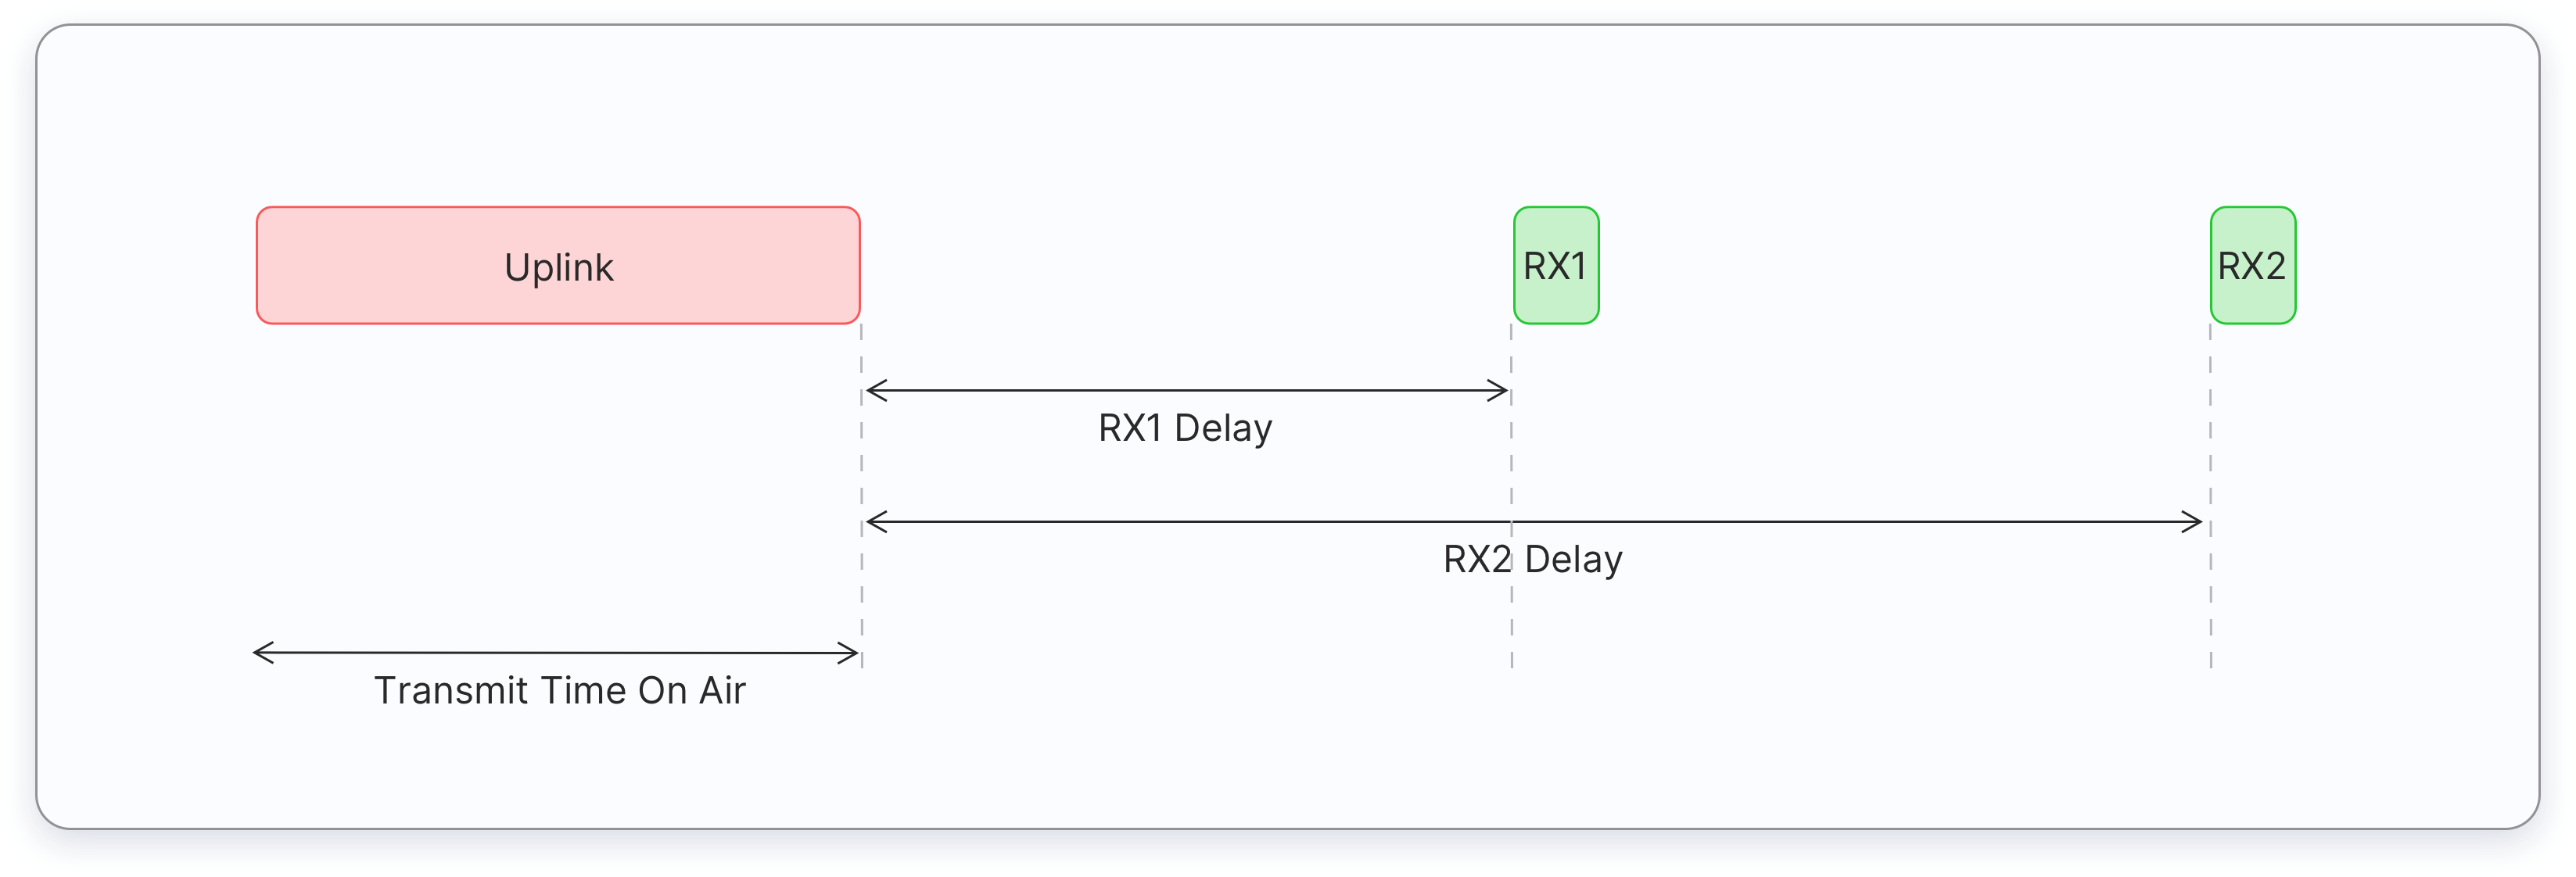
\includegraphics[width=0.8\textwidth]{figures/class-a.png}
    \caption{Operasi LoRaWAN Kelas A}
    \label{fig:lora_class_a}
\end{figure}
\begin{figure}
    \centering
    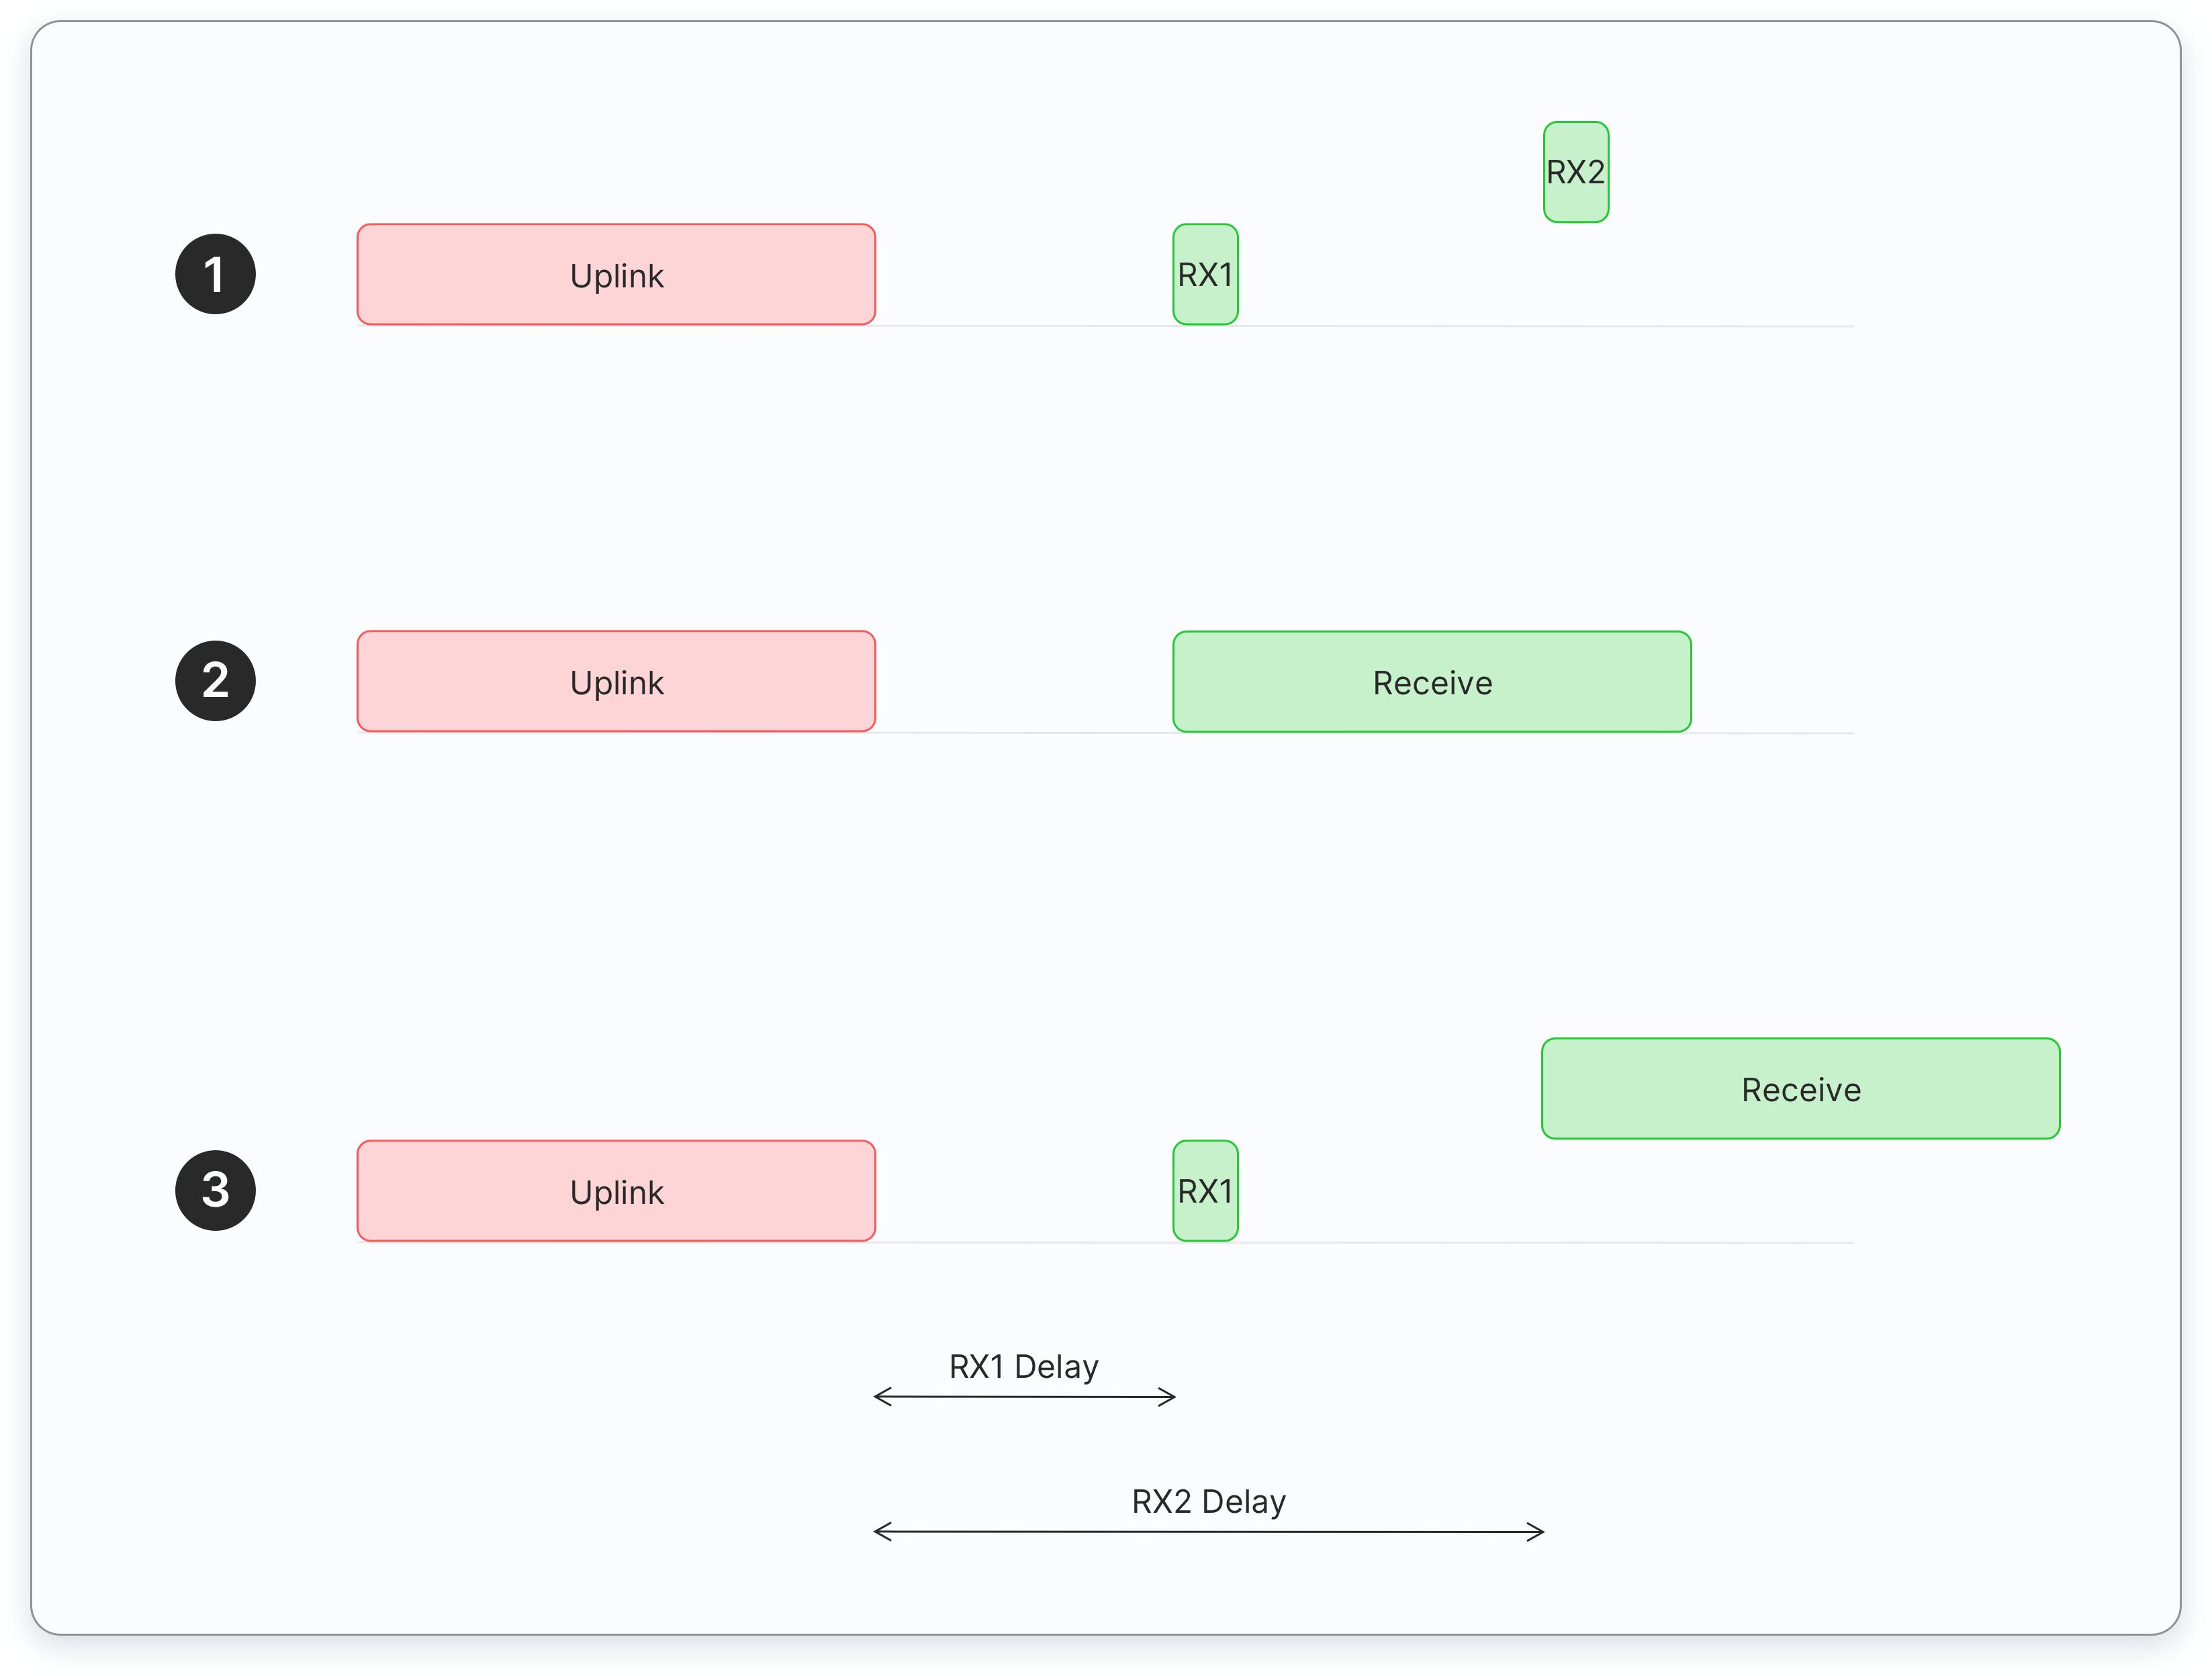
\includegraphics[width=0.8\textwidth]{figures/class-a-alt.png}
    \caption{Operasi Alternatif LoRaWAN Kelas A}
    \label{fig:lora_class_a_alt}
\end{figure}
Kelas A adalah kelas perangkat dasar dan wajib dalam LoRaWAN. Desainnya memprioritaskan konsumsi daya ultra-rendah, menjadikannya cocok untuk aplikasi berbaterai dengan kebutuhan komunikasi tidak sering.
Gambar~\ref{fig:lora_class_a} dan~\ref{fig:lora_class_a_alt} menggambarkan waktu transmisi uplink dan downlink dalam perangkat Kelas A.
\begin{enumerate}
    \item End-device dapat memulai transmisi uplink kapan saja.
    \item Setelah menyelesaikan transmisi uplink, perangkat membuka dua jendela penerimaan berurutan:
          \begin{enumerate}
              \item \textbf{RX1}: Dibuka setelah penundaan tetap (\texttt{RECEIVE\_DELAY1}, biasanya 1 detik).
              \item \textbf{RX2}: Dibuka setelah penundaan tetap kedua (\texttt{RECEIVE\_DELAY2}, biasanya 2 detik), yaitu 1 detik setelah RX1.
          \end{enumerate}
    \item Network Server dapat menjadwalkan downlink di RX1 atau RX2, tetapi tidak keduanya.
    \item Jika tidak ada downlink yang diterima di kedua jendela, kesempatan berikutnya untuk downlink hanya terjadi setelah perangkat mengirim uplink berikutnya.
    \item RX2 menggunakan frekuensi dan laju data tetap yang dikonfigurasi per parameter regional, sedangkan RX1 menggunakan saluran yang sama dengan uplink dan laju data yang diimbangi oleh \texttt{RX1DROffset}.
\end{enumerate}
Perangkat Kelas A menunjukkan latensi downlink tinggi tetapi mencapai efisiensi energi luar biasa dengan tetap dalam mode tidur antar transmisi. Aplikasi khas meliputi:
\begin{enumerate}
    \item Pemantauan lingkungan (misalnya, suhu, kelembaban, kualitas udara)
    \item Pelacakan hewan dan aset
    \item Deteksi kebakaran hutan dan kebocoran air
    \item Sistem parkir pintar dan manajemen limbah
\end{enumerate}
\subsection{Kelas B}
\begin{figure}
    \centering
    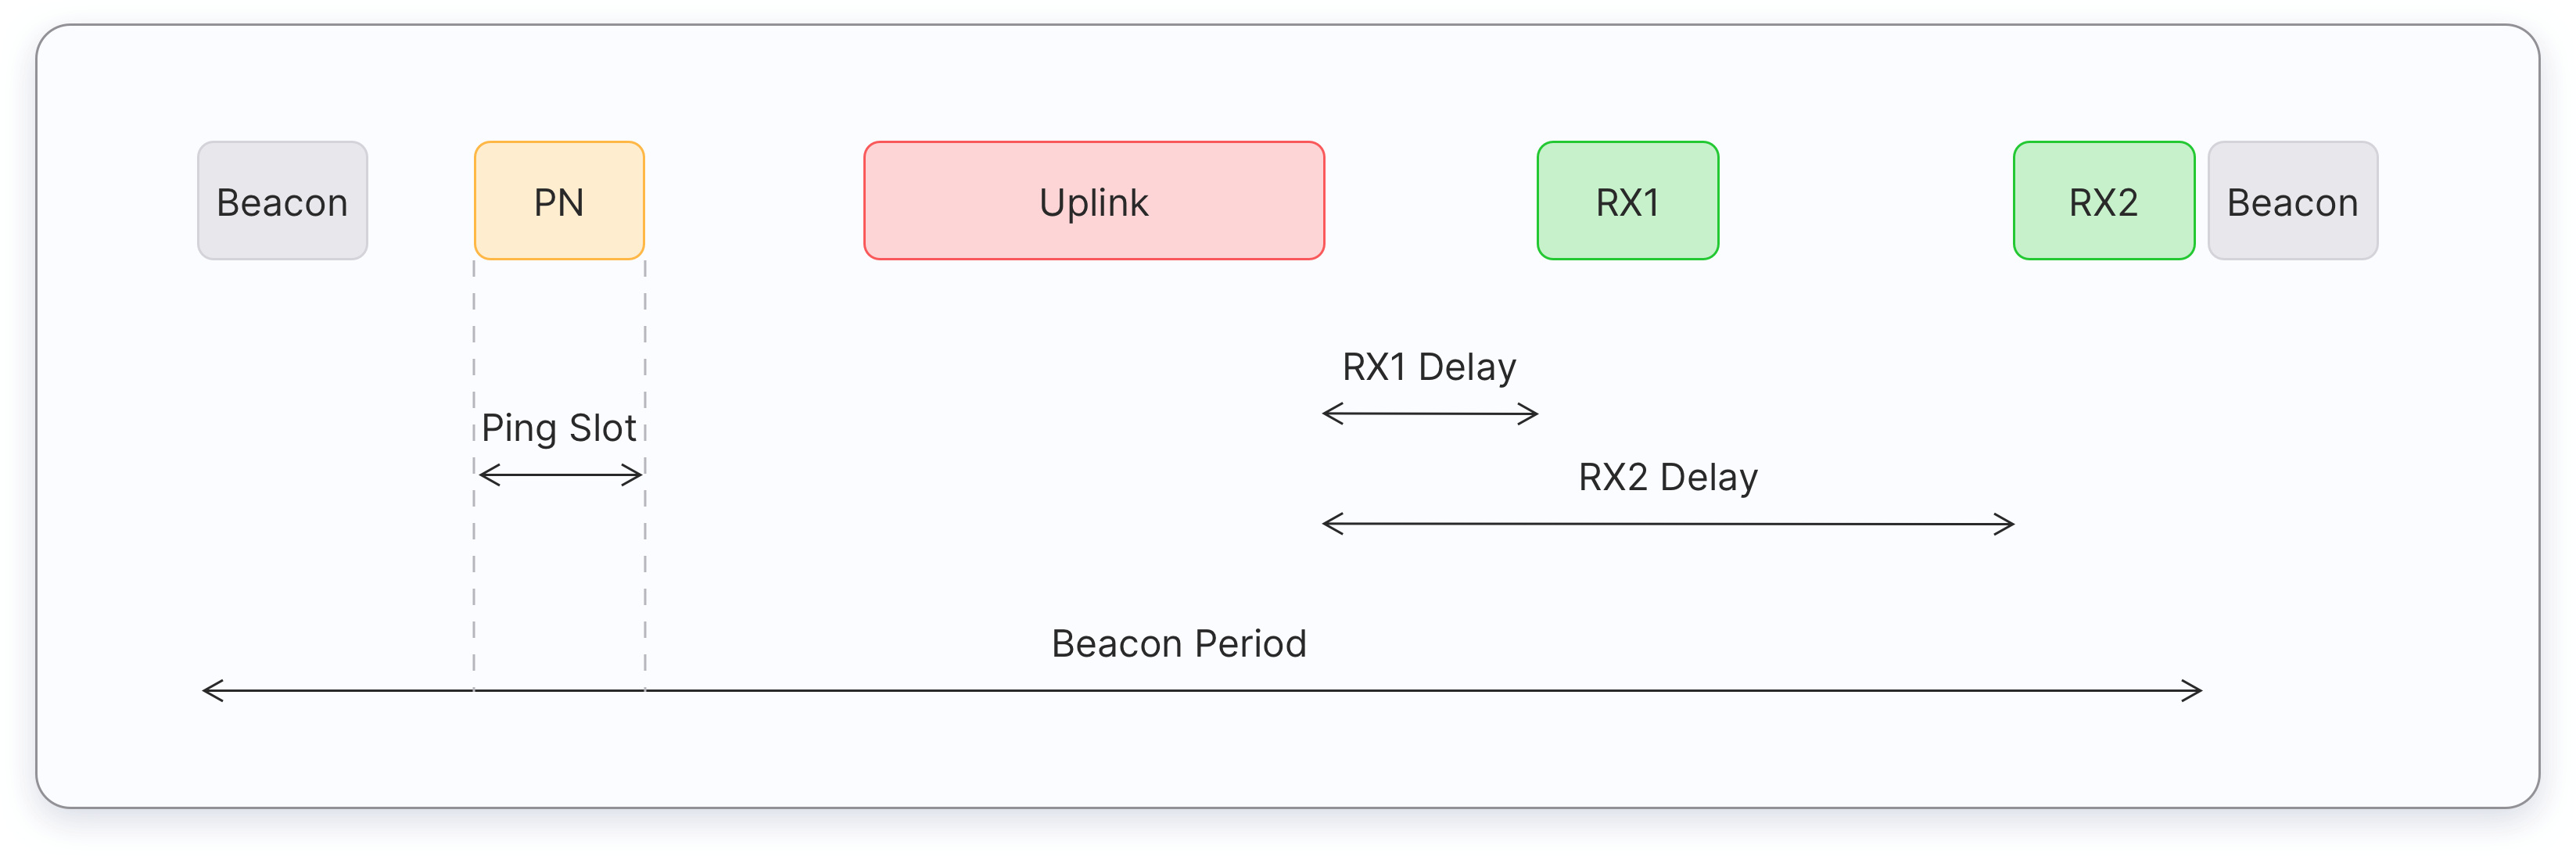
\includegraphics[width=0.8\textwidth]{figures/class-b.png}
    \caption{Operasi LoRaWAN Kelas B}
    \label{fig:lora_class_b}
\end{figure}
Kelas B memperluas Kelas A dengan memperkenalkan slot penerimaan terjadwal—dikenal sebagai \emph{ping slots}—untuk mengurangi latensi downlink sambil mempertahankan efisiensi daya yang wajar.
Gambar~\ref{fig:lora_class_b} menggambarkan waktu transmisi uplink dan downlink dalam perangkat Kelas B.
\begin{enumerate}
    \item Gateway secara berkala menyiarkan \emph{beacon} yang disinkronkan (setiap 128 detik secara default), yang memberikan referensi waktu umum.
    \item End-device menggunakan beacon ini untuk menyelaraskan jam internalnya dengan waktu jaringan.
    \item Berdasarkan sinkronisasi ini, Network Server dapat menjadwalkan downlink selama ping slots yang telah ditentukan untuk perangkat individual atau grup multicast.
    \item Setelah setiap uplink, perangkat masih membuka jendela RX1 dan RX2 seperti pada Kelas A.
    \item Ping slots terjadi pada interval reguler yang ditentukan oleh \texttt{PING\_SLOT\_PERIODICITY} (default: $2^7 = 128$ detik).
\end{enumerate}
Kelas B menawarkan latensi downlink sedang dan cocok untuk aplikasi yang memerlukan aktuasi sesekali atau interaksi downlink lebih sering daripada yang diizinkan Kelas A. Konsumsi daya lebih tinggi daripada Kelas A karena penerimaan beacon berkala dan pendengaran ping slot, tetapi banyak perangkat Kelas B tetap beroperasi dengan baterai dengan masa pakai yang dapat diterima.
Kasus penggunaan khas meliputi:
\begin{enumerate}
    \item Meteran utilitas (listrik, air, gas)
    \item Sistem pencahayaan jalan pintar
\end{enumerate}
Perangkat Kelas B dapat kembali ke operasi Kelas A ketika fungsionalitas ping slot tidak diperlukan.
\subsection{Kelas C}
\begin{figure}
    \centering
    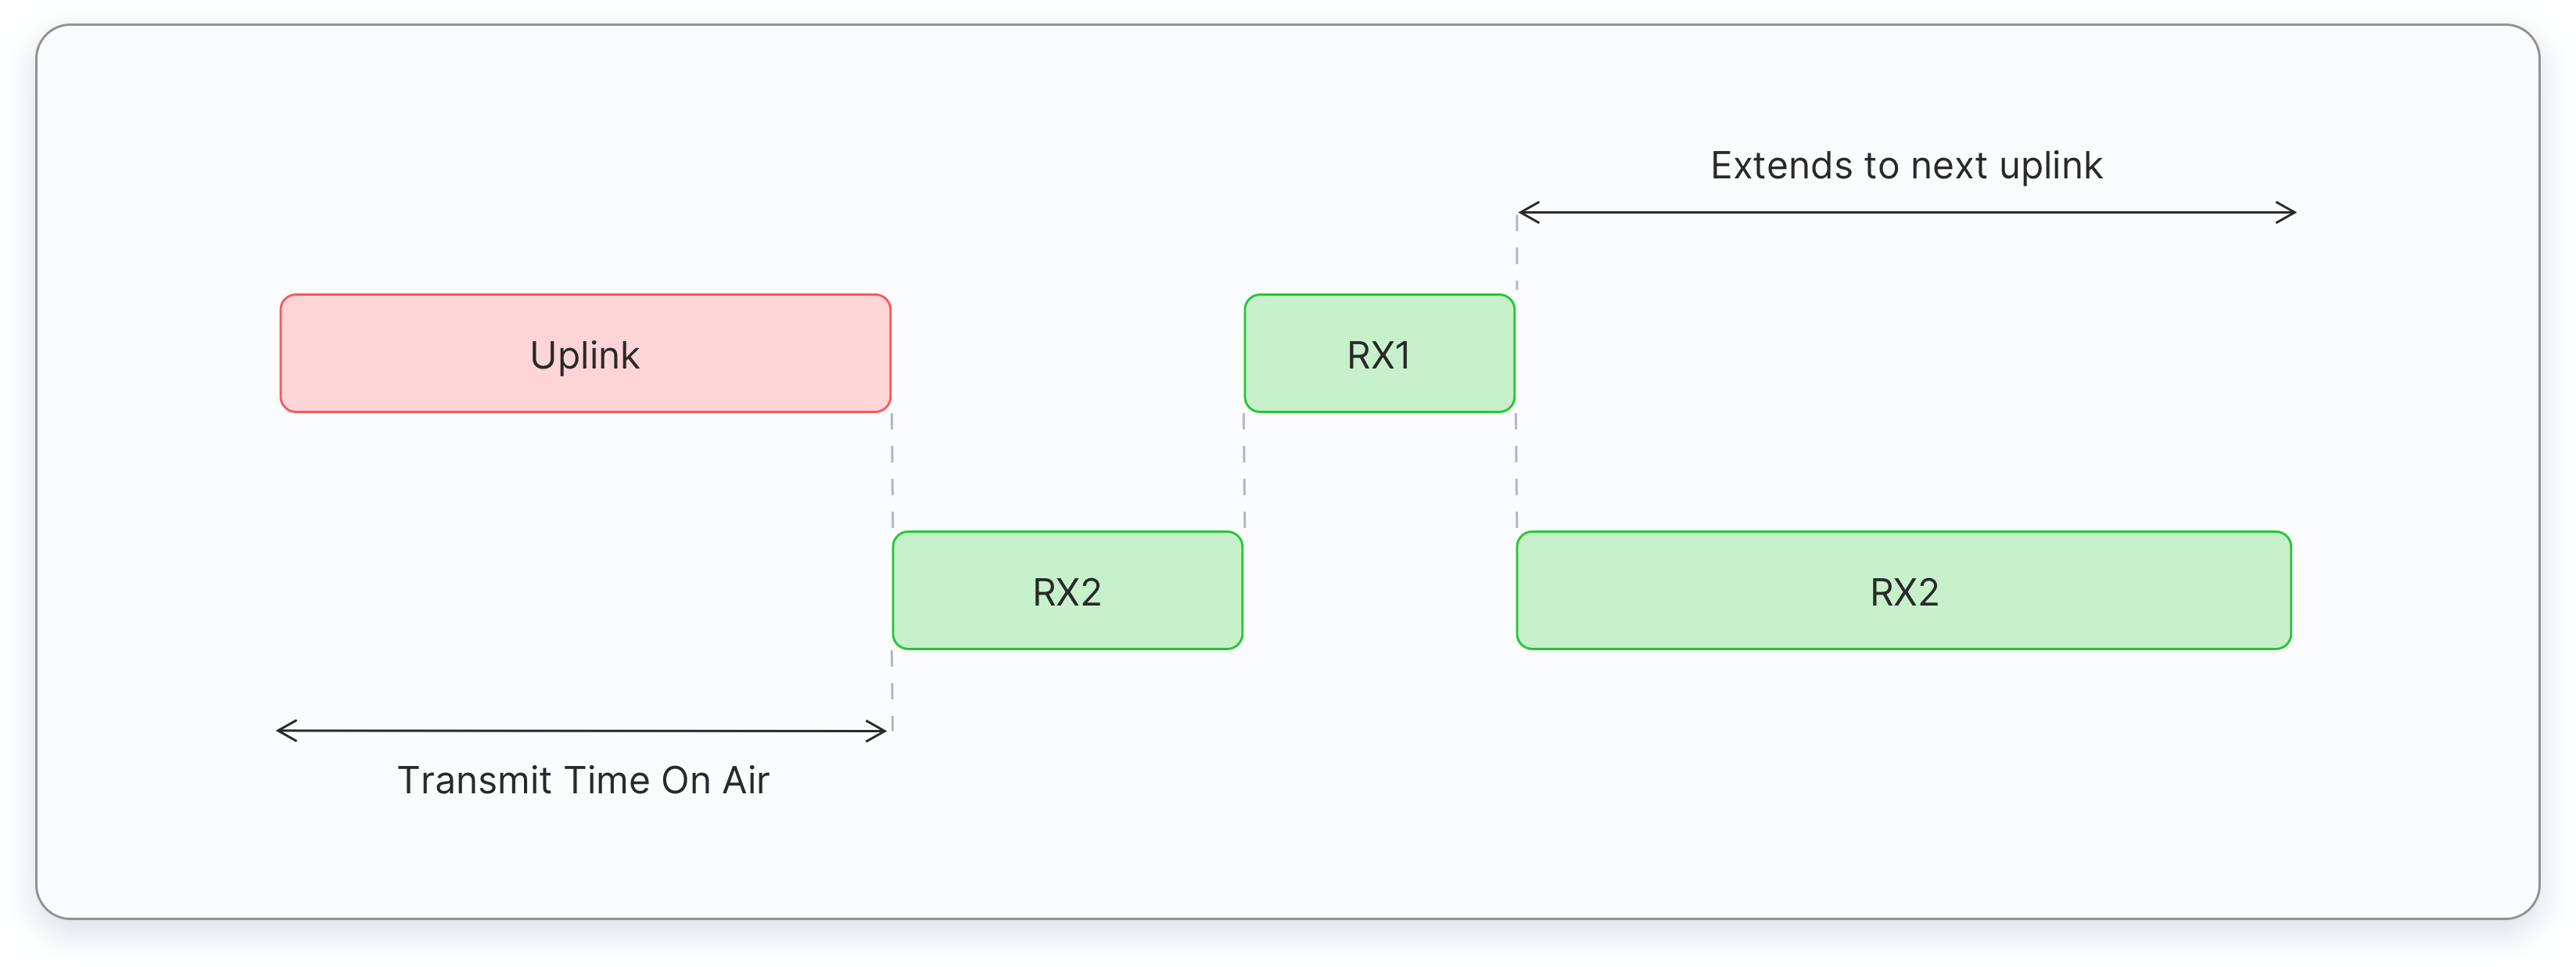
\includegraphics[width=0.8\textwidth]{figures/class-c.png}
    \caption{Operasi LoRaWAN Kelas C}
    \label{fig:lora_class_c}
\end{figure}
Kelas C memberikan latensi downlink serendah mungkin dengan menjaga penerima hampir selalu aktif, dengan mengorbankan konsumsi daya yang jauh lebih tinggi.
Gambar~\ref{fig:lora_class_c} menggambarkan waktu transmisi uplink dan downlink dalam perangkat Kelas C.
\begin{enumerate}
    \item Setelah transmisi uplink, perangkat membuka RX1 dan RX2 seperti pada Kelas A.
    \item Setelah RX2, perangkat menjaga jendela penerimaan RX2 \emph{terus terbuka} hingga transmisi uplink berikutnya dimulai.
    \item Ini memungkinkan Network Server mengirim pesan downlink kapan saja, hanya tunduk pada batasan duty cycle peraturan.
    \item Transmisi uplink hanya dimungkinkan ketika tidak ada downlink yang sedang berlangsung.
\end{enumerate}
Karena aktivitas radio yang hampir terus-menerus, perangkat Kelas C umumnya tidak cocok untuk operasi baterai jangka panjang dan biasanya menggunakan daya listrik.
Aplikasi umum meliputi:
\begin{enumerate}
    \item Meteran utilitas yang memerlukan kontrol real-time
    \item Lampu jalan dengan peredupan dinamis atau perintah hidup/mati
    \item Lampu suar dan sistem alarm yang memerlukan respons segera
\end{enumerate}
Perangkat Kelas C dapat beroperasi dalam mode Kelas A selama periode aktivitas rendah untuk menghemat energi, meskipun ini memerlukan peralihan mode eksplisit melalui perintah MAC atau logika aplikasi.
\section{Aktivasi End Device}
Sebelum berpartisipasi dalam jaringan LoRaWAN, setiap end device harus menjalani prosedur aktivasi untuk menetapkan kredensial kriptografi dan mendapatkan alamat jaringan. Dua metode aktivasi berbeda didefinisikan dalam spesifikasi LoRaWAN: Over-the-Air Activation (OTAA) dan Activation by Personalization (ABP). OTAA adalah pendekatan yang direkomendasikan dan lebih aman, memungkinkan turunan kunci dinamis dan roaming jaringan, sedangkan ABP melibatkan pra-konfigurasi kunci dan alamat statis, membatasi fleksibilitas dan keamanan.
\subsection{Over-the-Air Activation dalam LoRaWAN 1.0.x}
\begin{figure}[htbp]
    \centering
    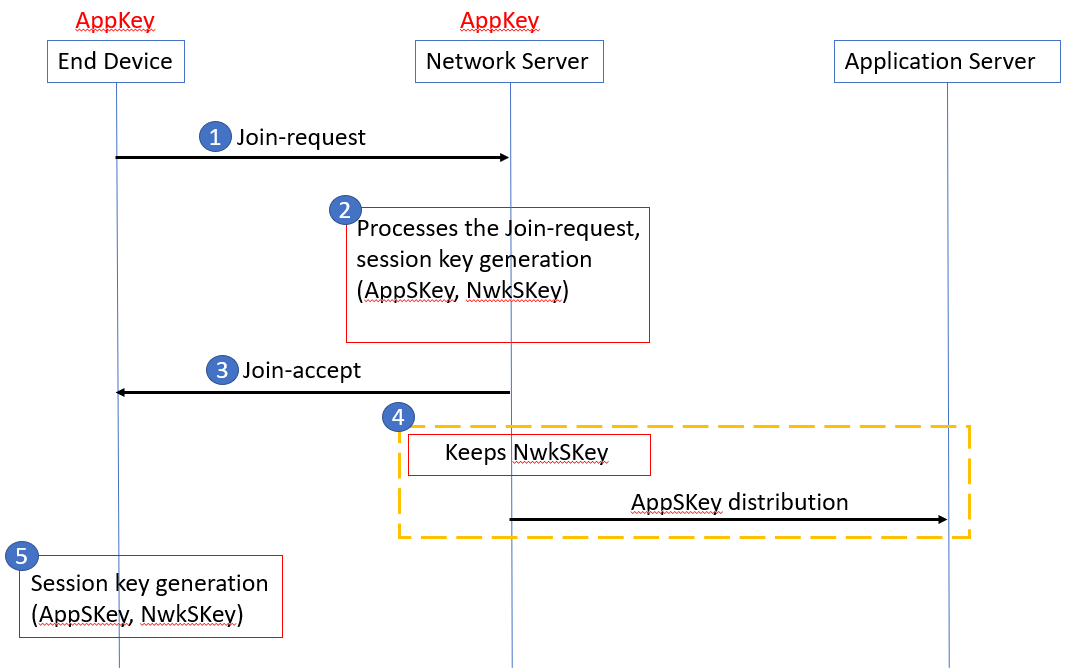
\includegraphics[width=0.8\textwidth]{figures/otaa-lorawan1.0.png}
    \caption{Prosedur Over-the-Air Activation (OTAA) LoRaWAN 1.0.x}
    \label{fig:lora_otaa_1.0}
\end{figure}
Dalam LoRaWAN 1.0.x, OTAA dicapai melalui jabat tangan dua pesan antara end device dan Network Server, difasilitasi oleh kunci root bersama. Prosedurnya adalah sebagai berikut:
Gambar~\ref{fig:lora_otaa_1.0} menggambarkan proses OTAA dalam LoRaWAN 1.0.x.
\begin{enumerate}
    \item \textbf{Prasyarat}: End device harus disediakan dengan parameter non-volatil berikut:
          \begin{enumerate}
              \item \texttt{AppEUI}: Pengenal IEEE EUI-64 64-bit dari server aplikasi.
              \item \texttt{DevEUI}: Pengenal unik IEEE EUI-64 64-bit dari end device.
              \item \texttt{AppKey}: Kunci root rahasia AES 128-bit, dibagikan dengan Network Server.
          \end{enumerate}
          \texttt{AppKey} tidak pernah dikirim melalui udara.
    \item \textbf{Transmisi Join-request}: End device memulai prosedur join dengan mengirimkan pesan \texttt{Join-request} yang berisi:
          \begin{enumerate}
              \item \texttt{AppEUI} (8 byte)
              \item \texttt{DevEUI} (8 byte)
              \item \texttt{DevNonce} (2 byte): nonce acak atau meningkat secara monoton untuk mencegah serangan replay.
          \end{enumerate}
          Message Integrity Code (MIC) dihitung berdasarkan field ini menggunakan \texttt{AppKey} dalam AES-CMAC. Pesan dikirim tanpa enkripsi pada salah satu saluran join spesifik wilayah (misalnya, 868.10/868.30/868.50 MHz dalam EU868).
    \item \textbf{Pembuatan Join-accept}: Setelah validasi berhasil, Network Server menghasilkan:
          \begin{enumerate}
              \item \texttt{DevAddr} dinamis 32-bit.
              \item Dua kunci sesi 128-bit: \texttt{NwkSKey} (untuk integritas lapisan jaringan dan enkripsi perintah MAC) dan \texttt{AppSKey} (untuk enkripsi payload aplikasi).
              \item Pesan \texttt{Join-accept} yang terdiri dari:
              \item \texttt{AppNonce} (3 byte): nonce yang disediakan server.
              \item \texttt{NetID} (3 byte): pengenal jaringan.
              \item \texttt{DevAddr} (4 byte)
              \item \texttt{DLSettings} (1 byte): konfigurasi downlink.
              \item \texttt{RxDelay} (1 byte): penundaan jendela penerimaan.
              \item \texttt{CFList} (0 atau 16 byte, opsional): frekuensi saluran tambahan.
          \end{enumerate}
          MIC dari \texttt{Join-accept} dihitung menggunakan \texttt{AppKey}, dan seluruh payload dienkripsi dengan \texttt{AppKey} menggunakan AES-128 dalam mode ECB.
    \item \textbf{Pengiriman Join-accept}: \texttt{Join-accept} yang dienkripsi dikirim ke end device melalui downlink di RX1 atau RX2. Tidak ada respons yang dikirim jika permintaan ditolak.
    \item \textbf{Turunan dan aktivasi kunci sesi}: End device mendekripsi \texttt{Join-accept} dan menurunkan \texttt{NwkSKey} dan \texttt{AppSKey} menggunakan \texttt{AppKey} dan \texttt{AppNonce}. Perangkat menyimpan:
          \begin{enumerate}
              \item \texttt{DevAddr}
              \item \texttt{NwkSKey}
              \item \texttt{AppSKey}
          \end{enumerate}
          Network Server menyimpan \texttt{NwkSKey}, sedangkan \texttt{AppSKey} diteruskan ke Application Server.
\end{enumerate}
\subsection{Over-the-Air Activation dalam LoRaWAN 1.1}
\begin{figure}[htbp]
    \centering
    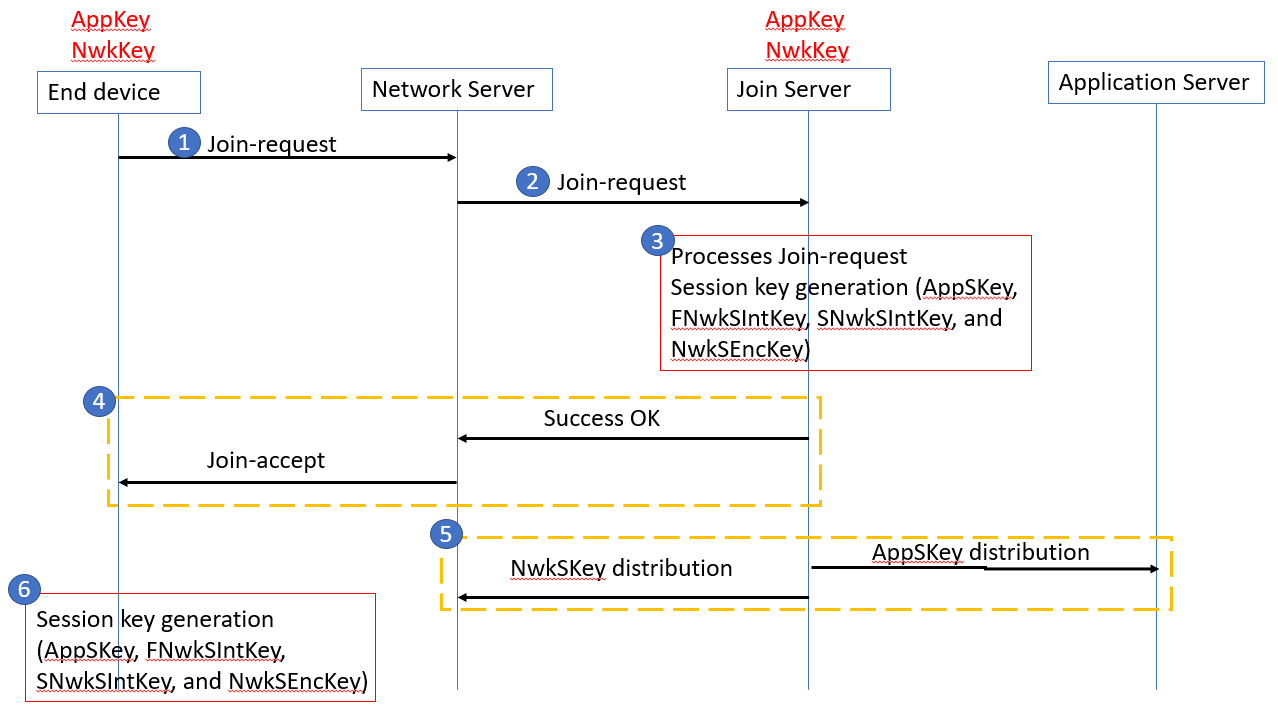
\includegraphics[width=0.8\textwidth]{figures/otaa-1.1.png}
    \caption{Prosedur Over-the-Air Activation (OTAA) LoRaWAN 1.1}
    \label{fig:lora_otaa_1.1}
\end{figure}
LoRaWAN 1.1 meningkatkan keamanan dengan memisahkan kunci root jaringan dan aplikasi serta memperkenalkan Join Server khusus. Prosedur OTAA melibatkan langkah-langkah berikut:
Gambar~\ref{fig:lora_otaa_1.1} menggambarkan proses OTAA dalam LoRaWAN 1.1.
\begin{enumerate}
    \item \textbf{Prasyarat}: End device disediakan dengan:
          \begin{enumerate}
              \item \texttt{JoinEUI}: Pengenal 64-bit dari Join Server (menggantikan \texttt{AppEUI}).
              \item \texttt{DevEUI}: Pengenal perangkat 64-bit.
              \item \texttt{AppKey}: Kunci root untuk turunan sesi aplikasi.
              \item \texttt{NwkKey}: Kunci root untuk turunan sesi jaringan.
          \end{enumerate}
          Kedua \texttt{AppKey} dan \texttt{NwkKey} dirahasiakan dan tidak pernah dikirim.
    \item \textbf{Transmisi Join-request}: End device mengirim \texttt{Join-request} yang berisi:
          \begin{enumerate}
              \item \texttt{JoinEUI} (8 byte)
              \item \texttt{DevEUI} (8 byte)
              \item \texttt{DevNonce} (2 byte): biasanya penghitung yang dinaikkan per upaya join.
          \end{enumerate}
          MIC dihitung menggunakan \texttt{NwkKey}. Pesan tidak dienkripsi dan dikirim pada saluran join spesifik wilayah.
    \item \textbf{Penerusan ke Join Server}: Network Server meneruskan \texttt{Join-request} yang divalidasi ke Join Server yang diidentifikasi oleh \texttt{JoinEUI}.
    \item \textbf{Pembuatan kunci sesi}: Join Server menurunkan empat kunci sesi:
          \begin{enumerate}
              \item \texttt{AppSKey}: untuk kerahasiaan payload aplikasi.
              \item \texttt{FNwkSIntKey}: untuk MIC uplink (bagian pertama).
              \item \texttt{SNwkSIntKey}: untuk MIC uplink (bagian kedua) dan semua MIC downlink.
              \item \texttt{NwkSEncKey}: untuk enkripsi perintah MAC dalam kedua arah.
          \end{enumerate}
    \item \textbf{Konstruksi dan enkripsi Join-accept}: Network Server menyusun pesan \texttt{Join-accept} dengan:
          \begin{enumerate}
              \item \texttt{JoinNonce} (1 byte): nonce yang disediakan Join Server.
              \item \texttt{NetID} (3 byte)
              \item \texttt{DevAddr} (4 byte)
              \item \texttt{DLSettings} (1 byte)
              \item \texttt{RxDelay} (1 byte)
              \item \texttt{CFList} (0 atau 16 byte, opsional)
          \end{enumerate}
          MIC dihitung menggunakan \texttt{JSIntKey} (diturunkan dari \texttt{NwkKey}), dan payload dienkripsi dengan \texttt{NwkKey} (untuk \texttt{Join-request}) atau \texttt{JSEncKey} (untuk \texttt{Rejoin-request}).
    \item \textbf{Distribusi kunci}: Join Server mengirim \texttt{AppSKey} ke Application Server dan tiga kunci jaringan (\texttt{FNwkSIntKey}, \texttt{SNwkSIntKey}, \texttt{NwkSEncKey}) ke Network Server.
    \item \textbf{Aktivasi perangkat}: End device mendekripsi \texttt{Join-accept} dan menurunkan keempat kunci sesi menggunakan \texttt{AppKey}, \texttt{NwkKey}, dan \texttt{JoinNonce}. Perangkat menyimpan:
          \begin{enumerate}
              \item \texttt{DevAddr}
              \item \texttt{AppSKey}
              \item \texttt{FNwkSIntKey}
              \item \texttt{SNwkSIntKey}
              \item \texttt{NwkSEncKey}
          \end{enumerate}
\end{enumerate}
\subsection{Activation by Personalization}
\begin{figure}
    \centering
    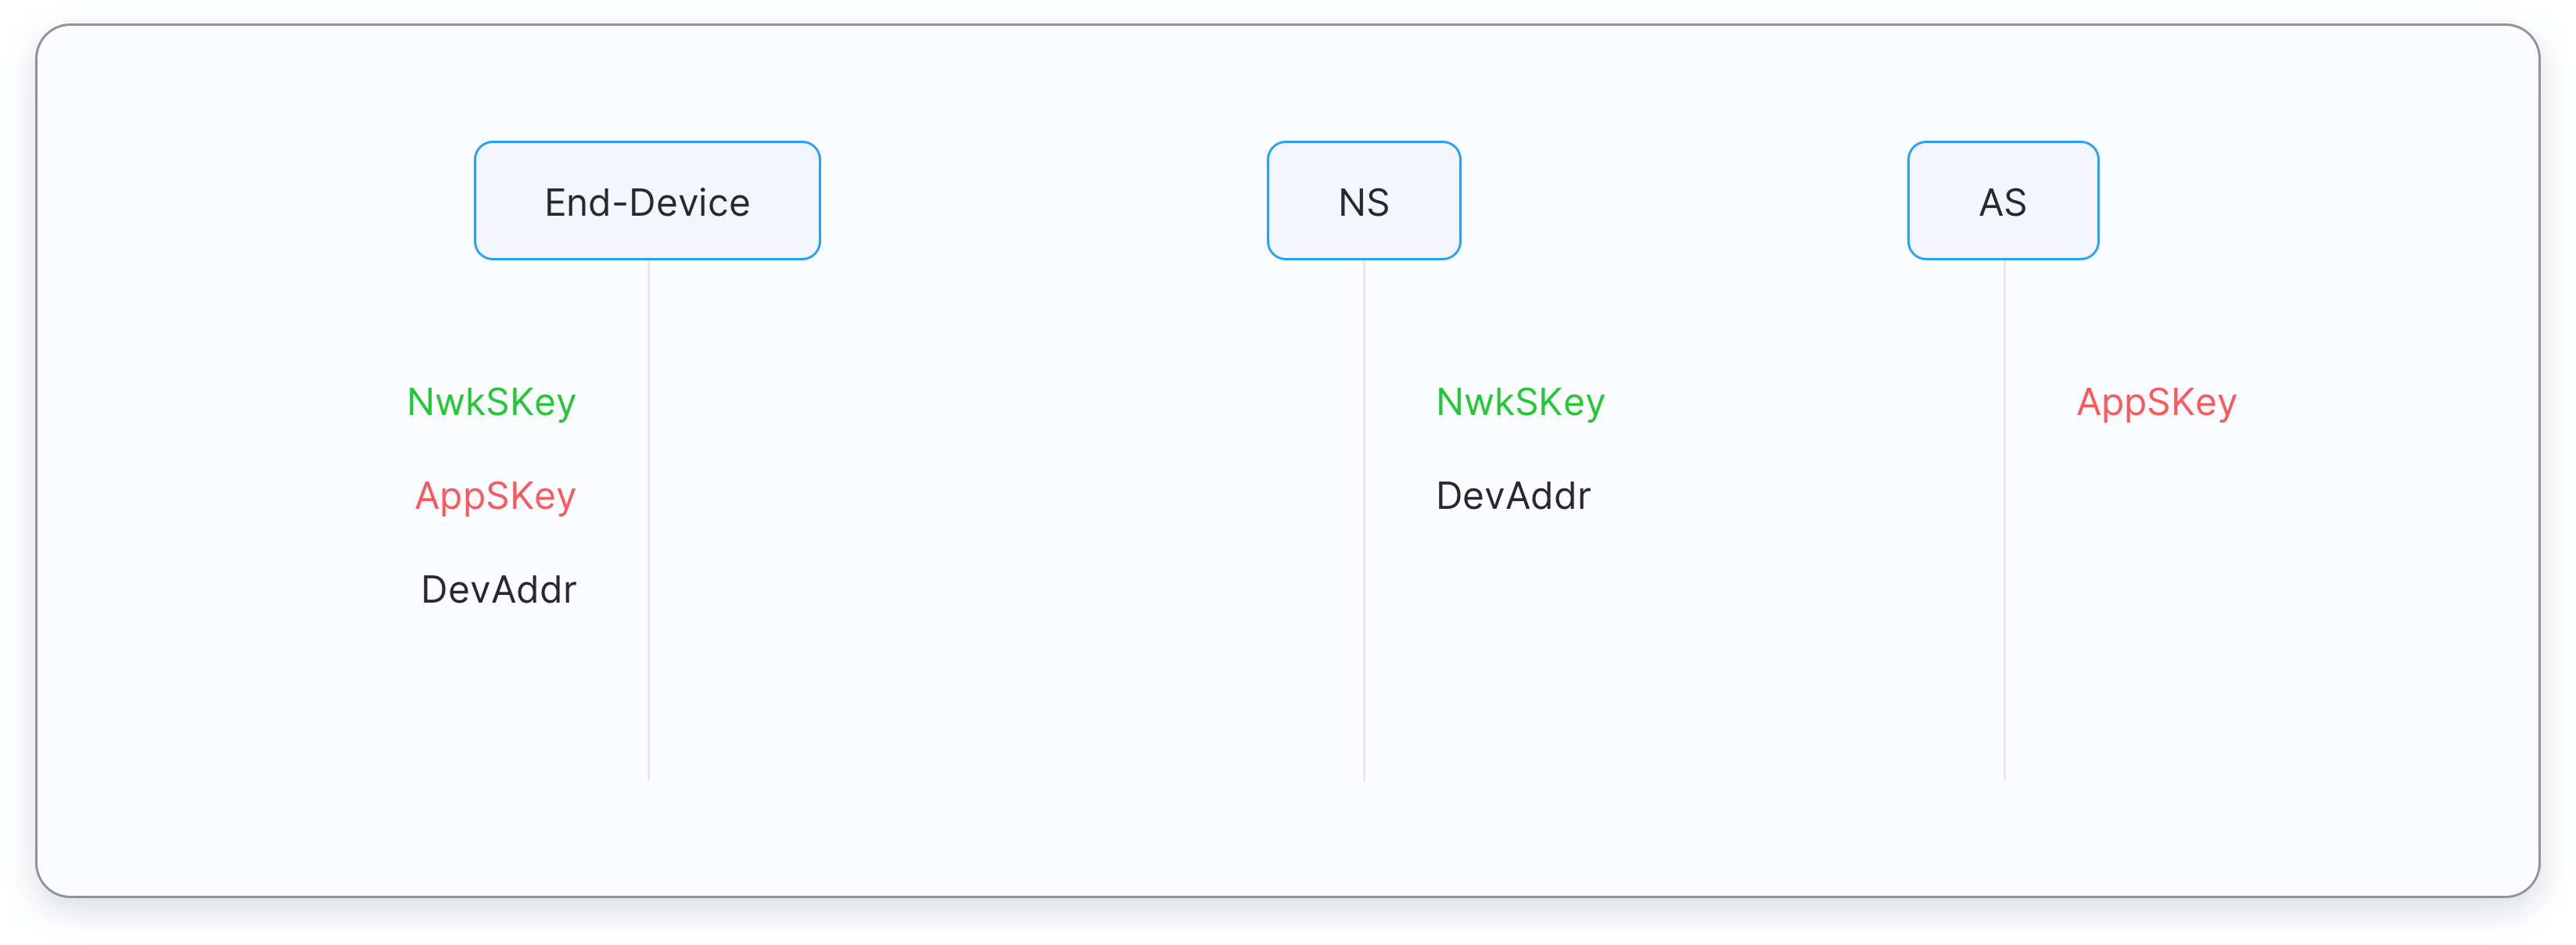
\includegraphics[width=0.8\textwidth]{figures/abp-1.0.png}
    \caption{Prosedur Activation by Personalization (ABP) LoRaWAN}
    \label{fig:lora_abp}
\end{figure}
Activation by Personalization (ABP) melewati prosedur join dengan mengonfigurasi parameter sesi langsung ke end device. Metode ini kurang aman dan tidak mendukung roaming jaringan.
Gambar~\ref{fig:lora_abp} menggambarkan proses ABP.
\begin{figure}
    \centering
    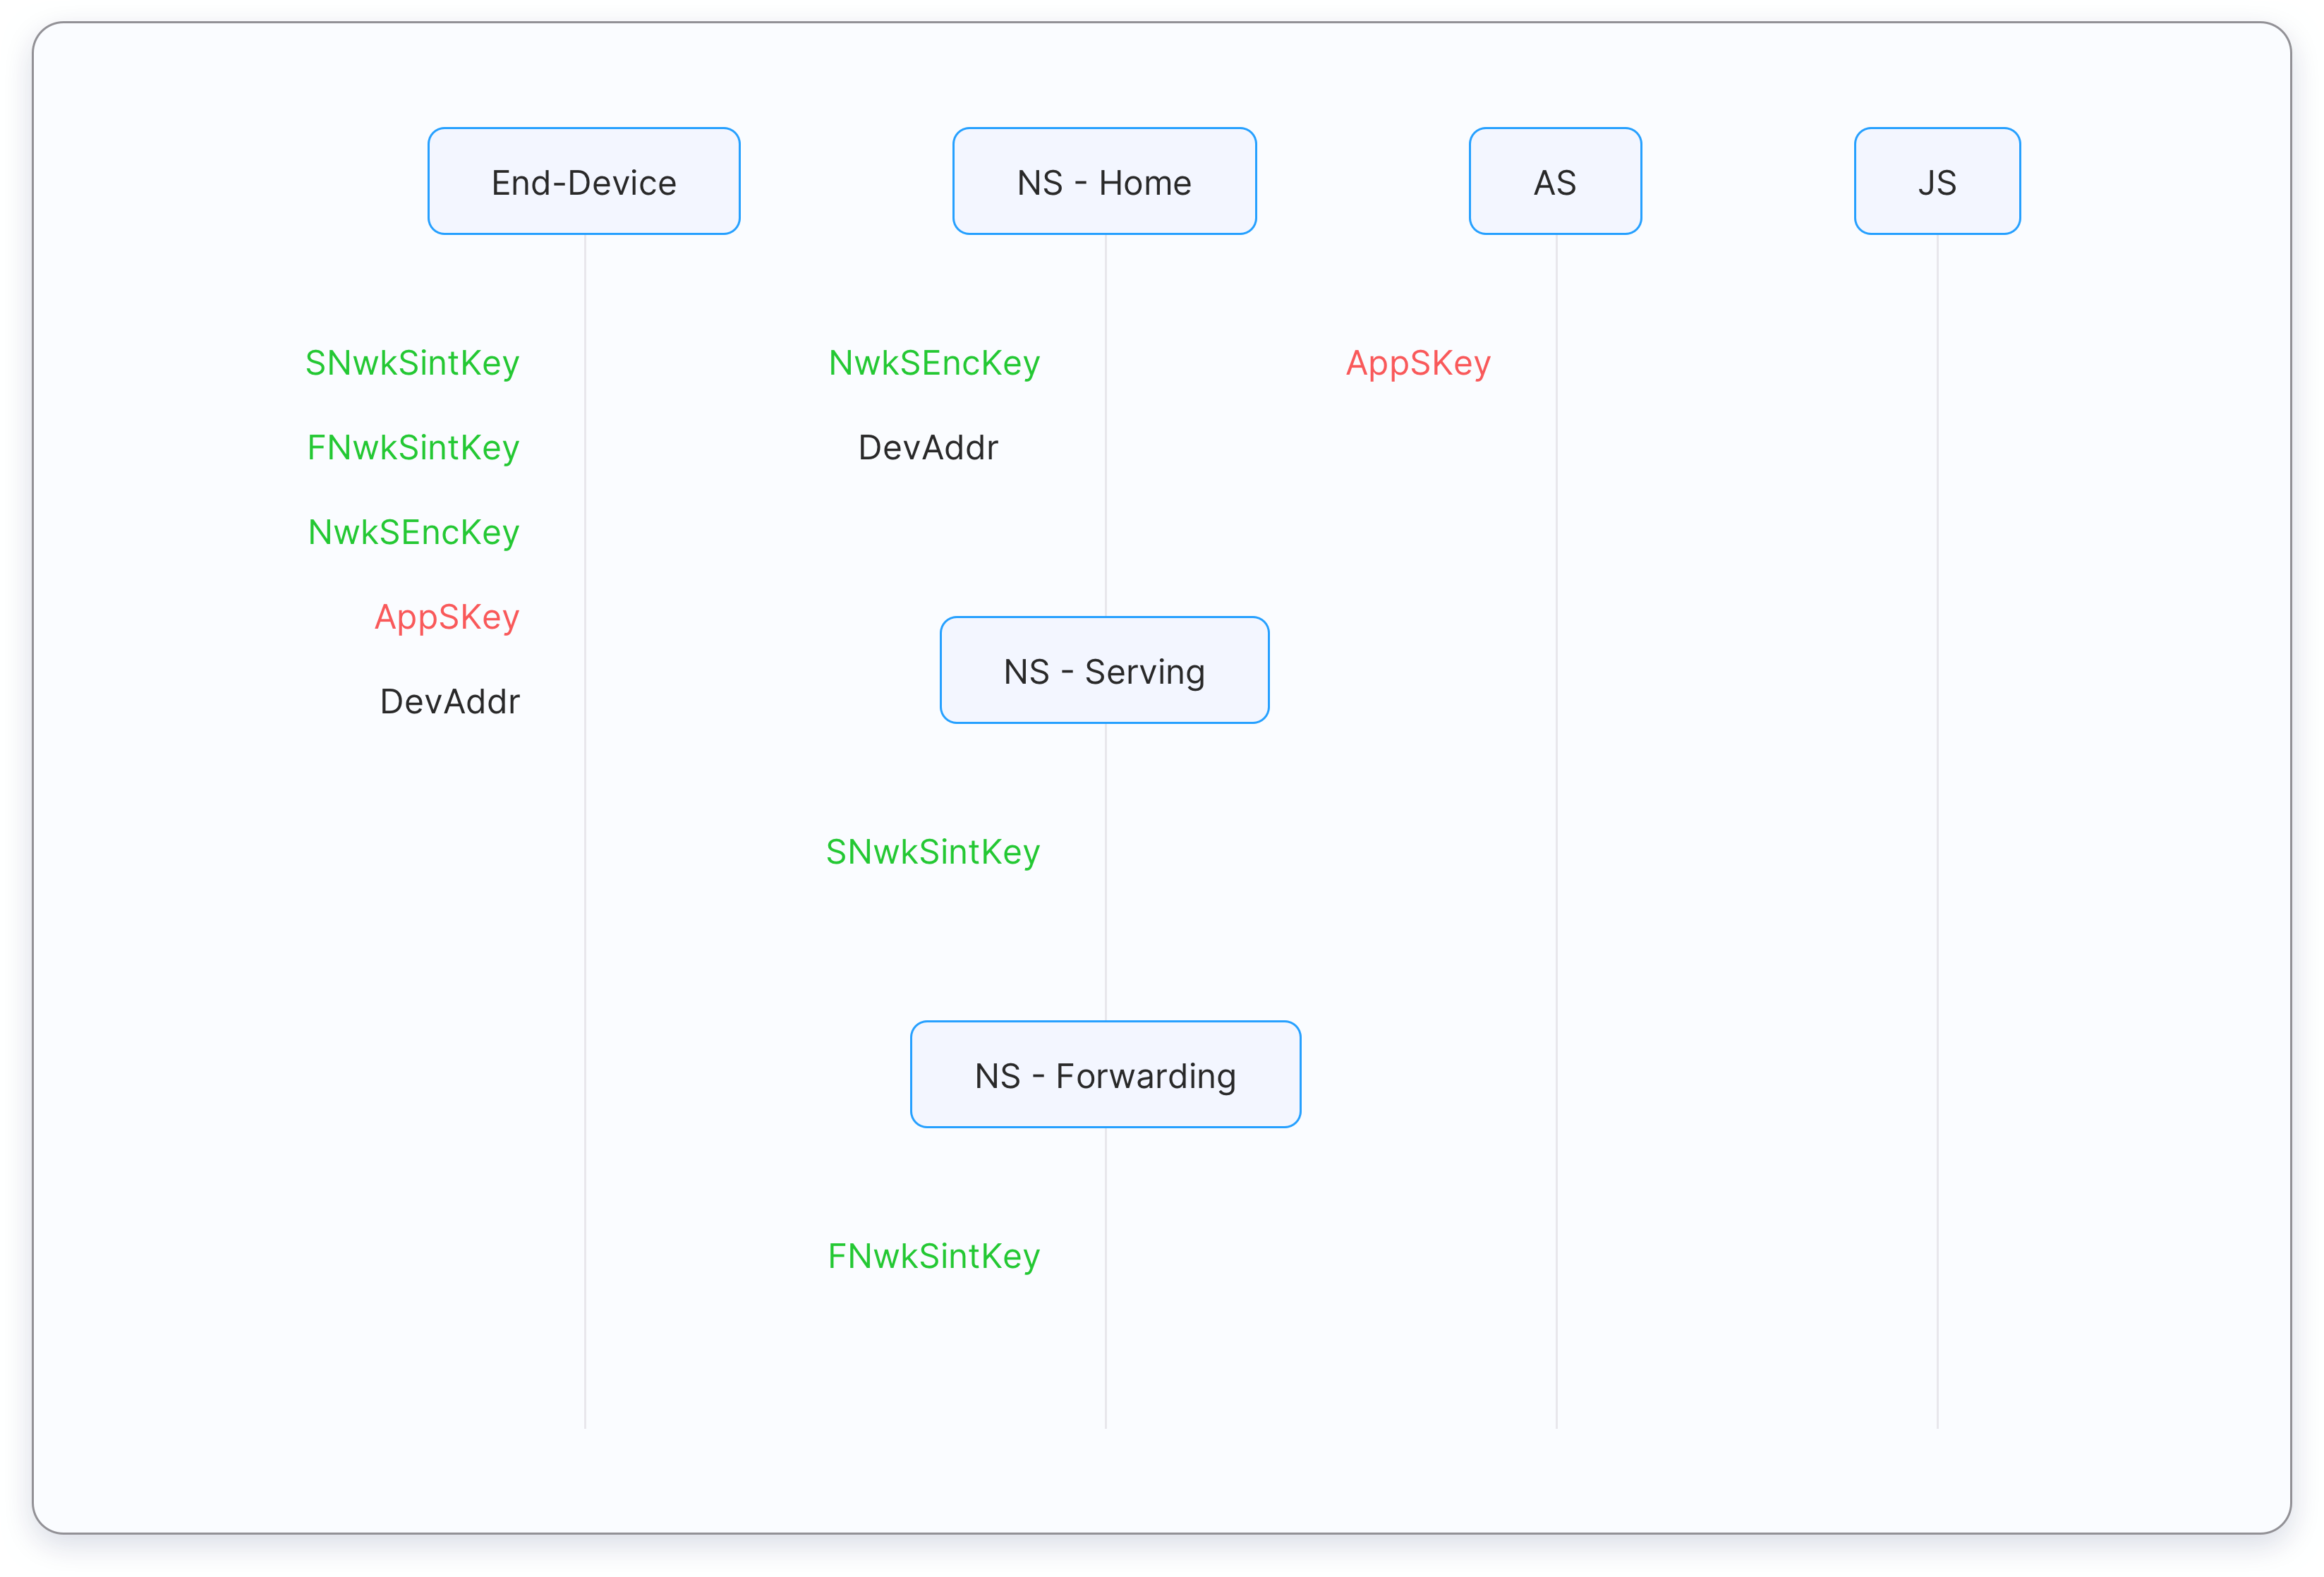
\includegraphics[width=0.8\textwidth]{figures/abp-1.1.png}
    \caption{Prosedur Activation by Personalization (ABP) LoRaWAN 1.1}
    \label{fig:lora_abp_1.1}
\end{figure}
Dalam LoRaWAN 1.1, ABP memerlukan pra-konfigurasi beberapa kunci sesi untuk menyelaraskan dengan model keamanan yang ditingkatkan.
Gambar~\ref{fig:lora_abp_1.1} menggambarkan proses ABP dalam LoRaWAN 1.1.
\begin{enumerate}
    \item \textbf{ABP dalam LoRaWAN 1.0.x}: Parameter berikut dipra-konfigurasi:
          \begin{enumerate}
              \item \texttt{DevAddr} (32 bit)
              \item \texttt{NwkSKey} (128 bit)
              \item \texttt{AppSKey} (128 bit)
          \end{enumerate}
          Parameter ini harus disinkronkan secara manual dengan Network Server (\texttt{DevAddr}, \texttt{NwkSKey}) dan Application Server (\texttt{AppSKey}).
    \item \textbf{ABP dalam LoRaWAN 1.1}: Empat kunci sesi dipra-konfigurasi:
          \begin{enumerate}
              \item \texttt{DevAddr} (32 bit)
              \item \texttt{FNwkSIntKey} (128 bit)
              \item \texttt{SNwkSIntKey} (128 bit)
              \item \texttt{NwkSEncKey} (128 bit)
              \item \texttt{AppSKey} (128 bit)
          \end{enumerate}
          Network Server menyimpan tiga kunci jaringan dan \texttt{DevAddr}, sedangkan Application Server menyimpan \texttt{AppSKey}.
    \item \textbf{Implikasi keamanan}: Perangkat ABP menggunakan kunci sesi statis sepanjang masa pakainya, meningkatkan kerentanan terhadap kompromi kunci. Selain itu, mengganti penyedia jaringan memerlukan rekonfigurasi manual semua materi kriptografi.
\end{enumerate}
\section{Spreading Factors}
LoRa menggunakan modulasi Chirp Spread Spectrum (CSS), di mana informasi dikodekan dalam pulsa yang dimodulasi frekuensi linear yang dikenal sebagai \emph{chirps} atau \emph{symbols}. \emph{Spreading factor} (SF) adalah parameter mendasar yang mengatur durasi dan struktur setiap chirp, sehingga secara langsung memengaruhi karakteristik transmisi utama termasuk laju data, jangkauan komunikasi, time-on-air, sensitivitas penerima, dan konsumsi energi.
\subsection{Definisi dan Dampak Spreading Factor}
\begin{enumerate}
    \item Spreading factor menentukan laju sapuan chirp: spreading factor yang lebih tinggi sesuai dengan chirp yang lebih lambat, yang meningkatkan durasi simbol dan mengurangi laju data.
    \item Untuk setiap kenaikan satu unit dalam spreading factor (misalnya, dari SF7 ke SF8), durasi chirp berlipat ganda, dan akibatnya laju data berkurang separuhnya untuk bandwidth dan laju pengkodean tetap.
    \item LoRa mendukung enam spreading factor, dilambangkan SF7 hingga SF12, di mana SF7 menghasilkan laju data tertinggi dan jangkauan terpendek, sedangkan SF12 memberikan laju data terendah dan jangkauan terpanjang.
    \item Spreading factor bersifat ortogonal: transmisi yang menggunakan spreading factor berbeda pada frekuensi yang sama dan pada waktu yang sama tidak saling mengganggu, memungkinkan penggunaan ulang spektrum dan manajemen kemacetan di jaringan padat.
\end{enumerate}
\subsection{Data Rate}
\begin{enumerate}
    \item Untuk bandwidth dan coding rate tetap, data rate berbanding terbalik dengan spreading factor.
    \item Data rate berbanding lurus dengan bandwidth: menggandakan bandwidth akan menggandakan data rate untuk spreading factor yang sama.
    \item Contoh bit rate untuk SF7 dengan coding rate 4/5 (sering disederhanakan sebagai CR = 1 dalam perhitungan nominal) adalah:
          \begin{enumerate}
              \item 5.5 kbit/s pada bandwidth 125 kHz
              \item 10.9 kbit/s pada bandwidth 250 kHz
              \item 21.9 kbit/s pada bandwidth 500 kHz
          \end{enumerate}
\end{enumerate}
\subsection{Communication Range}
\begin{enumerate}
    \item Spreading factor yang lebih tinggi meningkatkan processing gain, sehingga meningkatkan ketahanan sinyal terhadap noise dan memungkinkan penerimaan pada rasio signal-to-noise (SNR) yang lebih rendah.
    \item Akibatnya, transmisi yang menggunakan SF12 mencapai jangkauan yang jauh lebih besar dibandingkan dengan yang menggunakan SF7 dalam kondisi daya dan lingkungan yang identik.
    \item Sifat ini memungkinkan jaringan untuk secara dinamis menyesuaikan spreading factor per perangkat guna menyeimbangkan data rate dan jangkauan berdasarkan kualitas link.
\end{enumerate}
\subsection{Time-on-Air}
\begin{enumerate}
    \item Time-on-air mengacu pada durasi perangkat menduduki kanal untuk mentransmisikan payload tertentu.
    \item Untuk ukuran payload dan bandwidth tetap, time-on-air meningkat secara eksponensial seiring peningkatan spreading factor.
    \item Time-on-air yang lebih lama dapat memperparah keterbatasan duty cycle di pita frekuensi yang diatur dan meningkatkan kerentanan terhadap interferensi.
    \item Operator jaringan sering menggunakan kalkulator airtime (misalnya, LoRaWAN airtime calculator dari The Things Network) untuk memperkirakan durasi transmisi berdasarkan ukuran payload, bandwidth, dan spreading factor.
\end{enumerate}
\subsection{Receiver Sensitivity}
\begin{enumerate}
    \item Receiver sensitivity—daya sinyal minimum di mana penerima dapat mendekode transmisi dengan benar—meningkat dengan spreading factor yang lebih tinggi.
    \item Untuk bandwidth tetap 125 kHz, nilai receiver sensitivity tipikal adalah:
          \begin{enumerate}
              \item SF7: \SI{-123}{\decibel m}
              \item SF8: \SI{-126}{\decibel m}
              \item SF9: \SI{-129}{\decibel m}
              \item SF10: \SI{-132}{\decibel m}
              \item SF11: \SI{-134.5}{\decibel m}
              \item SF12: \SI{-137}{\decibel m}
          \end{enumerate}
    \item Peningkatan sensitivitas ini pada spreading factor tinggi sangat penting untuk menjaga konektivitas di lingkungan dengan sinyal rendah, seperti di dalam gedung atau area pedesaan.
\end{enumerate}
\subsection{Battery Life}
\begin{enumerate}
    \item Transmisi radio merupakan sumber utama konsumsi energi pada perangkat end LoRaWAN.
    \item Spreading factor yang lebih tinggi meningkatkan time-on-air, yang secara langsung meningkatkan waktu transmisi aktif dan konsumsi energi per pesan.
    \item Akibatnya, perangkat yang beroperasi terutama pada SF12 akan memiliki masa pakai baterai lebih pendek dibandingkan dengan perangkat yang beroperasi pada SF7, dengan asumsi ukuran payload dan frekuensi transmisi yang sama.
    \item Mekanisme Adaptive Data Rate (ADR) dalam LoRaWAN bertujuan untuk meminimalkan spreading factor (dan konsumsi daya) sambil mempertahankan keandalan link, sehingga mengoptimalkan umur baterai.
\end{enumerate}

\section{Adaptive Data Rate}
Adaptive Data Rate (ADR) adalah mekanisme yang dikendalikan jaringan yang dirancang untuk mengoptimalkan pertukaran antara keandalan komunikasi, pemanfaatan waktu udara (\emph{airtime}), dan konsumsi energi dalam jaringan LoRaWAN. Dengan menyesuaikan parameter transmisi secara dinamis berdasarkan kualitas tautan yang teramati, ADR memungkinkan penggunaan spektrum yang efisien sekaligus menjaga konektivitas yang andal.
\subsection{Transmission Parameters Controlled by ADR}
Mekanisme ADR mengatur parameter lapisan fisik berikut dari perangkat akhir:
\begin{enumerate}
    \item Spreading factor
    \item Bandwidth
    \item Transmission power
\end{enumerate}
Perangkat yang berada dekat dengan gateway biasanya beroperasi dengan spreading factor yang lebih rendah dan data rate yang lebih tinggi untuk meminimalkan airtime dan konsumsi energi. Sebaliknya, perangkat di tepi sel menggunakan spreading factor yang lebih tinggi untuk mencapai anggaran tautan (\emph{link budget}) yang diperlukan agar penerimaan tetap andal.
\subsection{Conditions for ADR Activation}
ADR sebaiknya hanya diaktifkan dalam kondisi frekuensi radio (RF) yang stabil. Oleh karena itu:
\begin{enumerate}
    \item Perangkat akhir statis umumnya dapat mengaktifkan ADR, asalkan lingkungan RF tetap konsisten.
    \item Jika perangkat statis mendeteksi degradasi RF sementara (misalnya karena adanya penghalang lingkungan seperti kendaraan yang diparkir di atas sensor), perangkat tersebut harus menonaktifkan ADR sementara.
    \item Perangkat akhir bergerak harus menerapkan logika untuk mendeteksi periode operasi stasioner yang berkepanjangan dan mengaktifkan ADR selama interval tersebut.
    \item Keputusan untuk mengaktifkan atau menonaktifkan ADR berada sepenuhnya pada perangkat akhir; baik server aplikasi maupun server jaringan tidak boleh mengesampingkan keputusan ini.
\end{enumerate}
\subsection{ADR Operation in The Things Stack}
The Things Stack mengimplementasikan ADR menggunakan algoritma optimasi berbasis pengukuran yang diturunkan dari strategi adaptasi laju yang direkomendasikan oleh Semtech. Aspek operasional utama meliputi:
\begin{enumerate}
    \item Saat bit ADR diatur dalam frame uplink, Network Server mulai mengumpulkan 20 pengukuran uplink terbaru. Setiap pengukuran mencakup:
          \begin{enumerate}
              \item Frame counter
              \item Signal-to-Noise Ratio (SNR) yang dilaporkan oleh gateway penerima terbaik
              \item Jumlah gateway yang menerima pesan tersebut
          \end{enumerate}
    \item Ketika bit ADR dibersihkan oleh perangkat (misalnya karena mobilitas atau kondisi RF yang tidak stabil), semua pengukuran sebelumnya dibuang. Pengumpulan pengukuran dilanjutkan hanya setelah bit ADR diaktifkan kembali.
    \item Untuk setiap pengukuran, \emph{margin} dihitung sebagai:
          \[
              \text{Margin} = \text{Measured SNR} - \text{Required SNR for current data rate}
          \]
          Margin ini mengkuantifikasi kelebihan anggaran tautan, yang menjadi dasar potensi peningkatan data rate atau pengurangan daya transmisi.
    \item Permintaan ADR dipicu dalam kondisi berikut:
          \begin{enumerate}
              \item \textbf{Initial ADR Request (hanya untuk US915 dan AU915)}: Dikirim segera setelah join dalam implementasi pra-LoRaWAN 1.1 untuk mengonfigurasi mask saluran. Permintaan ini mencakup margin keamanan karena pengukuran tautan belum mencukupi saat join. LoRaWAN 1.1 menghilangkan kebutuhan permintaan ini dengan memungkinkan konfigurasi mask saluran dalam pesan \texttt{JoinAccept}.
              \item \textbf{Regular ADR Request}: Dijadwalkan ketika pengukuran yang cukup menunjukkan pengaturan data rate atau daya yang tidak optimal. Permintaan ini disisipkan (\emph{piggybacked}) pada downlink lapisan aplikasi yang sudah ada (misalnya ACK atau payload).
              \item \textbf{Lowest Data Rate Trigger}: Dikirim ketika perangkat beroperasi pada DR0 (biasanya SF12/125 kHz), terlepas dari margin, untuk mendorong adaptasi laju.
              \item \textbf{ADR Acknowledgment Request}: Dipicu ketika perangkat mengatur bit \texttt{ADRAckReq}, biasanya setelah mengirim 64 uplink tanpa menerima downlink (tergantung implementasi).
          \end{enumerate}
    \item Jika perangkat akhir berulang kali menolak perintah ADR, Network Server akan berhenti menjadwalkan permintaan ADR lebih lanjut. Perilaku ini dapat mengindikasikan adanya masalah firmware perangkat atau ketidakcocokan versi antara perangkat dan server.
\end{enumerate}
\section{Limitations and Design Recommendations}
LoRaWAN adalah protokol Low Power Wide Area Network (LPWAN) khusus yang dioptimalkan untuk kelas aplikasi Internet of Things (IoT) tertentu. Meskipun menawarkan keunggulan signifikan dalam hal jangkauan, efisiensi energi, dan biaya, protokol ini secara inheren tidak cocok untuk kasus penggunaan yang memerlukan data rate tinggi, latensi rendah, atau komunikasi kontinu. Memahami keterbatasan ini sangat penting untuk desain sistem dan pemanfaatan sumber daya yang efektif.
\subsection{Appropriate Use Cases for LoRaWAN}
LoRaWAN cocok untuk aplikasi yang memiliki karakteristik berikut:
\begin{enumerate}
    \item \textbf{Komunikasi jarak jauh}: Mampu mencapai cakupan beberapa kilometer di lingkungan pedesaan dan ratusan meter hingga beberapa kilometer di lingkungan perkotaan.
    \item \textbf{Konsumsi daya sangat rendah}: Perangkat akhir dapat beroperasi selama beberapa tahun dengan satu baterai berkat operasi berbasis duty cycle dan mode tidur yang efisien.
    \item \textbf{Biaya modal dan operasional rendah}: Biaya perangkat keras biasanya di bawah 20\,\texteuro\ per node, dengan biaya operasional berulang yang minimal.
    \item \textbf{Kebutuhan data rate rendah}: Laju bit lapisan fisik berkisar antara sekitar 250\,bit/s hingga 11\,kbit/s di pita EU868 (menggunakan modulasi LoRa), tergantung pada spreading factor dan bandwidth yang dipilih.
    \item \textbf{Penyebaran jaringan terdesentralisasi}: Pengguna dapat menyebar gateway pribadi untuk mencapai cakupan di area terpencil atau kurang terlayani tanpa bergantung pada infrastruktur pihak ketiga.
    \item \textbf{Keamanan end-to-end}: Semua payload aplikasi dienkripsi menggunakan AES 128-bit, menjamin kerahasiaan dan integritas.
\end{enumerate}
\subsection{Inappropriate Use Cases for LoRaWAN}
LoRaWAN tidak dirancang untuk skenario berikut:
\begin{enumerate}
    \item \textbf{Transmisi data real-time atau frekuensi tinggi}: Protokol ini menerapkan duty cycle regulasi dan dioptimalkan untuk transmisi infrekuensi (misalnya sekali setiap beberapa menit).
    \item \textbf{Komunikasi suara atau audio}: Teknologi seperti GPRS, 3G, atau LTE lebih sesuai untuk layanan berbasis suara.
    \item \textbf{Sistem kendali jarak pendek dengan interaksi tinggi}: Protokol seperti Zigbee atau Bluetooth Low Energy (BLE) lebih cocok untuk otomasi rumah (misalnya pengendalian pencahayaan).
    \item \textbf{Aplikasi bandwidth tinggi}: Transmisi gambar, streaming video (misalnya Netflix), atau file besar tidak layak; Wi-Fi atau broadband seluler sebaiknya digunakan sebagai gantinya.
\end{enumerate}
\subsection{Uplink Transmission Best Practices}
Untuk memaksimalkan efisiensi spektrum, masa pakai baterai, dan kapasitas jaringan, pedoman berikut harus diperhatikan untuk komunikasi uplink:
\begin{enumerate}
    \item \textbf{Minimalkan ukuran payload}: Data harus dikodekan dalam format biner ringkas, bukan representasi verbose seperti JSON atau teks ASCII. Format Cayenne Low Power Payload (LPP) direkomendasikan karena kesederhanaan dan dukungan luasnya.
    \item \textbf{Optimalkan frekuensi transmisi}: Pesan harus dikirim dengan interval beberapa menit. Strategi agregasi data—seperti melaporkan nilai minimum, rata-rata, dan maksimum selama suatu jendela—atau transmisi berbasis peristiwa (misalnya dipicu oleh pelanggaran ambang batas atau deteksi gerakan) dapat secara signifikan mengurangi lalu lintas yang tidak perlu.
    \item \textbf{Gunakan data rate tertinggi yang memungkinkan}: Data rate yang lebih tinggi (misalnya SF7 dengan bandwidth 125\,kHz) meminimalkan time-on-air dan konsumsi energi. Jika margin tautan tidak mencukupi, spreading factor dapat ditingkatkan secara bertahap. Adaptive Data Rate (ADR) harus diaktifkan jika kondisi RF stabil, memungkinkan server jaringan untuk mengoptimalkan data rate dan daya transmisi secara dinamis.
\end{enumerate}
\subsection{Downlink Transmission Best Practices}
Karena sifat half-duplex dari sebagian besar gateway LoRaWAN, transmisi downlink sementara menonaktifkan kemampuan gateway untuk menerima pesan uplink di semua saluran. Hal ini berdampak pada kapasitas dan keandalan jaringan. Oleh karena itu, batasan berikut berlaku:
\begin{enumerate}
    \item \textbf{Minimalkan penggunaan downlink}: Pesan downlink harus dihindari kecuali benar-benar diperlukan untuk fungsionalitas aplikasi.
    \item \textbf{Jaga agar payload downlink tetap kecil}: Jika downlink diperlukan, ukuran payload harus diminimalkan untuk mengurangi airtime.
    \item \textbf{Optimalkan uplink untuk meningkatkan efisiensi downlink}: Data rate downlink diturunkan dari data rate uplink dan RX1DROffset. Konfigurasi uplink yang efisien (misalnya data rate tinggi) memungkinkan downlink yang lebih efisien pula.
    \item \textbf{Hindari uplink confirmed kecuali benar-benar diperlukan}: Pesan uplink confirmed memicu acknowledgment downlink wajib, meningkatkan beban jaringan. Aplikasi harus dirancang untuk mentolerir kehilangan pesan sesekali bila memungkinkan, menggunakan mekanisme keandalan lapisan aplikasi jika diperlukan.
\end{enumerate}
\chapter{Metode Penelitian}

\section{Campus-Based LoRaWAN Architecture with Basic Station Gateway}
\label{subsec:campus_lorawan_architecture}

\begin{figure}[htbp]
    \centering
    % Replace with your actual image file (e.g., exported as PNG or PDF from draw.io)
    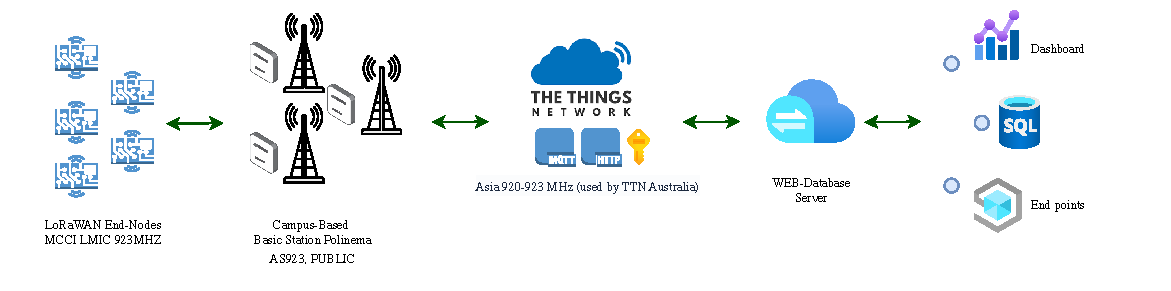
\includegraphics[width=0.95\textwidth]{../figures/cb-iot-arch.drawio.pdf}
    \caption{Campus-based LoRaWAN architecture using Basic Station gateway compliant with AS923 (Indonesia).}
    \label{fig:campuslorawanarch}
\end{figure}

Figure~\ref{fig:campuslorawanarch} illustrates the proposed campus-scale LoRaWAN architecture deployed at Polinema, utilizing the Basic Station gateway model compliant with Indonesian regulatory requirements. The system integrates end-devices, a LoRaWAN gateway, cloud infrastructure, and application endpoints into a cohesive IoT test bed. The components and data flow are described as follows:

\begin{enumerate}
    \item \textbf{LoRaWAN End-Nodes}
          \begin{enumerate}
              \item Located on the left side of the diagram, these represent sensor or actuator devices deployed across the campus (e.g., environmental monitors, smart meters).
              \item Each end-node is implemented using the MCCI LMIC stack configured for the \texttt{AS923} frequency plan (920–923 MHz), in accordance with Permenkominfo No. 21/2019.
              \item Devices transmit uplink messages using LoRa modulation and adhere to the 10\% duty cycle and 14 dBm EIRP power limit mandated for Indonesia.
          \end{enumerate}

    \item \textbf{Basic Station Gateway (Campus-Based)}
          \begin{enumerate}
              \item Positioned at the center-left, the gateway is labeled \textit{Campus-Based Basic Station Polinema} and operates in the \texttt{AS923 (PUBLIC)} mode.
              \item The gateway hardware (e.g., SenseCAP M1 or equivalent) runs the Basic Station software stack, enabling secure communication with The Things Network (TTN) via WebSocket over TLS.
              \item It receives LoRa frames from multiple end-nodes simultaneously across different spreading factors and channels within the 920–923 MHz band.
              \item The gateway forwards all received packets to the LoRaWAN Network Server (LNS) in the cloud using the LNS protocol, while also receiving downlink commands via the same secure channel.
          \end{enumerate}

    \item \textbf{Cloud Infrastructure (The Things Network)}
          \begin{enumerate}
              \item Represented by the central cloud icon, this layer corresponds to TTN’s \texttt{au1} or \texttt{eu1} cluster (configured as \texttt{AS923} for compatibility with Indonesian devices).
              \item The LNS performs frame validation, deduplication, and routing of application data to the appropriate integration endpoints.
              \item The gateway authenticates with TTN using its unique Gateway EUI and an API key, ensuring secure and authorized traffic exchange.
          \end{enumerate}

    \item \textbf{Application and Data Endpoints}
          \begin{enumerate}
              \item On the right side, three primary endpoints are shown:
                    \begin{enumerate}
                        \item \textit{Dashboard}: A web-based monitoring interface (e.g., Grafana, TTN Console) for real-time visualization of sensor data.
                        \item \textit{Time Series Data Sets}: A database or time-series storage system (e.g., InfluxDB, Azure Time Series Insights) for historical data logging and analytics.
                        \item \textit{Web-Database Server}: A custom application server hosting business logic, user management, and RESTful APIs for campus services (e.g., smart lighting, occupancy tracking).
                    \end{enumerate}
              \item Data flows from TTN to these endpoints via HTTP/MQTT integrations, as indicated by the protocol icons (HTTP, MQTT, and policy/access symbols) above the cloud layer.
          \end{enumerate}

    \item \textbf{Data Flow and Protocols}
          \begin{enumerate}
              \item Bidirectional arrows between components indicate full-duplex communication:
                    \begin{enumerate}
                        \item End-nodes $\leftrightarrow$ Gateway: LoRa RF communication (920–923 MHz, AS923).
                        \item Gateway $\leftrightarrow$ TTN: Secure WebSocket (port 8887) using Basic Station LNS protocol.
                        \item TTN $\leftrightarrow$ Endpoints: Standard internet protocols (HTTP/HTTPS, MQTT over TLS).
                    \end{enumerate}
              \item All cloud-to-application links are encrypted and authenticated, ensuring end-to-end security from sensor to dashboard.
          \end{enumerate}
\end{enumerate}

This architecture enables scalable, secure, and regulatory-compliant IoT deployment across the Polinema campus. By leveraging Basic Station and TTN, the system supports remote gateway management, over-the-air updates, and seamless integration with existing campus IT infrastructure—making it suitable for both research and operational use cases.



\section{Configuring Gateway: Basic Station}
\label{sec:configuring_gateway_basic_station}

This section provides a step-by-step guide to configuring a LoRaWAN gateway using the Basic Station software stack on The Things Network (TTN). The instructions are tailored for the Seeed Studio SenseCAP M1 gateway, which natively supports Basic Station and offers a user-friendly WebUI for initial setup.

\subsection{Setting-up Basic Station on TTN}
\label{subsec:basic_station_ttn_setup}

To integrate a Basic Station-compatible gateway (such as the SenseCAP M1) with The Things Network (TTN), the following steps must be performed. These steps assume the gateway has internet connectivity and has been powered on.

\begin{enumerate}
    \item \textbf{Create a Gateway Entry in The Things Network Console}
          \begin{enumerate}
              \item Log in to your account at \url{https://console.cloud.thethings.network/}.
              \item Navigate to the desired application or create a new one if necessary.
              \item In the left-hand menu, click on \textit{Gateways} and then select \textit{+ Add gateway}.
              \item Fill in the required fields:
                    \begin{enumerate}
                        \item \textit{Gateway ID}: Enter a unique, lowercase identifier (e.g., \texttt{univ-campus-gw-01}). This ID must be globally unique across TTN.
                        \item \textit{Gateway EUI}: Enter the 64-bit Gateway EUI (typically printed on the device label or found in the WebUI under device information). It must be entered in hexadecimal format without colons or dashes (e.g., \texttt{ABCDEF1234567890}).
                        \item \textit{Gateway Server Address}: Set to \texttt{eu1.cloud.thethings.network} (or the appropriate cluster region, e.g., \texttt{nam1}, \texttt{au1}, etc.).
                        \item \textit{Frequency Plan}: Select the correct regional plan. For Indonesia, choose \texttt{AS923} (specifically \texttt{AS923 - Group 1} or as defined by local regulations).
                        \item Leave other fields at their default values unless advanced configuration is required.
                    \end{enumerate}
              \item Click \textit{Create gateway}.
          \end{enumerate}

    \item \textbf{Obtain Gateway Authentication Credentials}
          \begin{enumerate}
              \item After creating the gateway, navigate to the gateway’s overview page in the TTN Console.
              \item Go to the \textit{General Settings} tab.
              \item Scroll down to the \textit{Gateway Authentication} section.
              \item Click \textit{Generate API key}.
              \item In the pop-up window:
                    \begin{enumerate}
                        \item Provide a name for the key (e.g., \texttt{basic-station-key}).
                        \item Under \textit{Rights}, ensure at least the following permissions are selected:
                              \begin{enumerate}
                                  \item \texttt{View gateway information}
                                  \item \texttt{Link as Gateway to a Gateway Server for traffic exchange}
                              \end{enumerate}
                        \item Click \textit{Create API key}.
                    \end{enumerate}
              \item Copy the generated API key immediately—it will not be shown again.
          \end{enumerate}

    \item \textbf{Configure the Gateway to Use TTN as LNS}
          \begin{enumerate}
              \item The SenseCAP M1 uses Basic Station, which requires two server endpoints:
                    \begin{enumerate}
                        \item \textit{LNS (LoRa Network Server)}: For real-time packet forwarding (e.g., \texttt{wss://[cluster].cloud.thethings.network:8887}).
                        \item \textit{CUPS (Configuration and Update Server)}: For secure provisioning and updates (e.g., \texttt{https://[cluster].cloud.thethings.network:443}).
                    \end{enumerate}
              \item These endpoints are typically configured automatically via the WebUI when TTN is selected as the network provider (see next subsection).
              \item The Gateway EUI and API key obtained above are used by the gateway to authenticate with TTN’s LNS and CUPS services.
          \end{enumerate}
\end{enumerate}

\subsection{Configuring Basic Station SenseCAP M1: WEBUI}
\label{subsec:sensecap_m1_webui}

The SenseCAP M1 provides a built-in web-based user interface (WebUI) accessible over Wi-Fi or Ethernet. The following steps detail the configuration process through this interface.

\begin{enumerate}
    \item \textbf{Access the WebUI}
          \begin{enumerate}
              \item Power on the SenseCAP M1 gateway.
              \item Connect your computer or mobile device to the gateway’s default Wi-Fi hotspot (SSID typically starts with \texttt{SenseCAP\_M1\_XXXX}).
              \item Open a web browser and navigate to \url{http://192.168.100.1}.
              \item Log in using the default credentials (usually username: \texttt{admin}, password: printed on the device label or set during first boot).
          \end{enumerate}

    \item \textbf{Connect to Local Network}
          \begin{enumerate}
              \item In the WebUI, go to \textit{Network Settings}.
              \item Configure internet connectivity:
                    \begin{enumerate}
                        \item For Wi-Fi: Select your campus or lab Wi-Fi network and enter the password.
                        \item For Ethernet: Ensure a cable is connected; DHCP is enabled by default.
                    \end{enumerate}
              \item Save settings and wait for the gateway to obtain an IP address on the local network.
              \item Note the new local IP address (e.g., \texttt{192.168.1.50}) to access the WebUI from the local network.
          \end{enumerate}

    \item \textbf{Select Network Provider}
          \begin{enumerate}
              \item Navigate to \textit{LoRaWAN Settings} or \textit{Network Provider}.
              \item Choose \textit{The Things Network (TTN)} from the list of available providers.
              \item The WebUI will automatically populate the following fields:
                    \begin{enumerate}
                        \item LNS Server: \texttt{wss://[region].cloud.thethings.network:8887}
                        \item CUPS Server: \texttt{https://[region].cloud.thethings.network:443}
                    \end{enumerate}
              \item If your region is not auto-detected, manually select the correct TTN cluster (e.g., \texttt{eu1} for Europe, \texttt{nam1} for North America). For Indonesia, \texttt{au1} or \texttt{eu1} may be used depending on latency and policy.
          \end{enumerate}

    \item \textbf{Enter Gateway Credentials}
          \begin{enumerate}
              \item In the same \textit{LoRaWAN Settings} section, enter the following:
                    \begin{enumerate}
                        \item \textit{Gateway EUI}: The 16-character hexadecimal EUI registered in TTN (e.g., \texttt{ABCDEF1234567890}).
                        \item \textit{API Key}: Paste the API key generated in Subsection~\ref{subsec:basic_station_ttn_setup}.
                    \end{enumerate}
              \item Ensure the \textit{Frequency Plan} is set to \texttt{AS923} to comply with Indonesian regulations (Permenkominfo No. 21/2019).
              \item Optionally, adjust the \textit{Transmission Power} and \textit{Duty Cycle} settings to respect the 14 dBm EIRP limit and 10\% duty cycle requirement for the 920–923 MHz band.
          \end{enumerate}

    \item \textbf{Apply and Reboot}
          \begin{enumerate}
              \item Click \textit{Save} or \textit{Apply Configuration}.
              \item The gateway will restart and initiate a secure WebSocket connection to TTN’s LNS using TLS.
              \item Monitor the WebUI status page for connection indicators (e.g., “Connected to LNS”).
          \end{enumerate}

    \item \textbf{Verify Operation in TTN Console}
          \begin{enumerate}
              \item Return to the TTN Console gateway page.
              \item Check the \textit{Live Data} tab to confirm uplink messages are being received.
              \item Verify that the gateway status shows as \textit{Connected}.
              \item If no data appears, check:
                    \begin{enumerate}
                        \item Internet connectivity of the gateway,
                        \item Correctness of Gateway EUI and API key,
                        \item Regional frequency plan alignment (AS923 for Indonesia),
                        \item Firewall or proxy settings that may block WebSocket (port 8887) or HTTPS (port 443) traffic.
                    \end{enumerate}
          \end{enumerate}
\end{enumerate}


\section{End-Nodes Using Lilygo T3S3}
\label{sec:end_nodes_lilygo_t3s3}
The end-nodes for this campus-based LoRaWAN architecture are implemented using the Lilygo T3S3 development board, which features the ESP32 microcontroller and an integrated SX1276 LoRa transceiver. The following outlines the configuration and programming steps to set up the Lilygo T3S3 as LoRaWAN end-nodes compliant with the AS923 frequency plan.
\subsection{Hardware Setup}
\begin{enumerate}
    \item \textbf{Lilygo T3S3 Board}
          \begin{enumerate}
              \item Ensure you have the Lilygo T3S3 board with the SX1276 LoRa module.
              \item Connect the board to your computer via USB for programming and power.
          \end{enumerate}
    \item \textbf{Antenna Connection}
          \begin{enumerate}
              \item Attach a suitable antenna for the 920–923 MHz frequency range to the LoRa module to ensure optimal signal transmission and reception.
          \end{enumerate}
\end{enumerate}
\subsection{Software Setup}
\begin{enumerate}
    \item \textbf{Arduino IDE Configuration}
          \begin{enumerate}
              \item Install the Arduino IDE if not already installed.
              \item Add the ESP32 board support by including the following URL in the Additional Board Manager URLs: \url{https://dl.espressif.com/dl/package_esp32_index.json}.
              \item Install the ESP32 board package via the Board Manager.
              \item Select the Lilygo T3S3 board from the Tools > Board menu.
          \end{enumerate}
    \item \textbf{Library Installation}
          \begin{enumerate}
              \item Install the MCCI LoRaWAN LMIC library via the Library Manager (Sketch > Include Library > Manage Libraries).
              \item Ensure the library version supports the AS923 frequency plan.
          \end{enumerate}
\end{enumerate}
\subsection{Programming the End-Nodes}
\begin{enumerate}
    \item \textbf{LoRaWAN Configuration}
          \begin{enumerate}
              \item Configure the LMIC library for the AS923 frequency plan by defining the appropriate parameters in your sketch.
              \item Set the device EUI, application EUI, and application key as provided by TTN for your end-node.
          \end{enumerate}
    \item \textbf{Uplink Message Implementation}
          \begin{enumerate}
              \item Implement code to read sensor data (e.g., temperature, humidity) and format it into a payload suitable for LoRaWAN transmission.
              \item Use the LMIC library functions to send uplink messages at defined intervals, adhering to duty cycle regulations.
          \end{enumerate}
    \item \textbf{Testing and Deployment}
          \begin{enumerate}
              \item Upload the sketch to the Lilygo T3S3 board.
              \item Monitor the TTN Console to verify that uplink messages are being received correctly.
              \item Deploy the end-nodes across the campus as needed, ensuring they are within range of the gateway.
          \end{enumerate}
\end{enumerate}

\subsection{LoRaWAN TTN End-Device Registration}
To register the Lilygo T3S3 end-nodes on The Things Network (TTN), follow these steps:
\begin{enumerate}
    \item Log in to your TTN Console account.
    \item Navigate to the application where you want to register the end-device.
    \item Click on \textit{End devices} and then select \textit{+ Add end device}.
    \item Fill in the required fields:
          \begin{enumerate}
              \item \textit{End device ID}: A unique identifier for the end-device (e.g., \texttt{lilygo-t3s3-node-01}).
              \item \textit{Device EUI}: The 64-bit unique identifier for the device, which can be generated or obtained from the board.
              \item \textit{Application EUI}: The 64-bit identifier for the application, provided by TTN.
              \item \textit{App Key}: A 128-bit key used for encryption, also provided by TTN.
              \item \textit{Frequency Plan}: Select \texttt{AS923} to comply with Indonesian regulations.
              \item Leave other fields at their default values unless specific configurations are needed.
              \item Click \textit{Create end device}.
              \item Repeat the process for each Lilygo T3S3 end-node you wish to register.
              \item After registration, monitor the \textit{Live Data} tab for each end-device to verify successful uplink message reception.
              \item Ensure that the end-nodes are configured to use OTAA (Over-The-Air Activation) for secure network joining.
              \item Deploy the end-nodes in their intended locations and ensure they are within range of the gateway for optimal performance.
          \end{enumerate}
\end{enumerate}

Table~\ref{tab:TTN_frequency_plans} summarizes the frequency plans available on TTN, highlighting the AS923 plan used in this architecture.
\begin{table}[htbp]
    \centering
    \caption{TTN Frequency Plans Summary}
    \label{tab:TTN_frequency_plans}
    \begin{tabular}{|c|c|c|c|}
        \hline
        \textbf{Frequency Plan} & \textbf{Region}          & \textbf{Uplink Frequencies (MHz)} & \textbf{Downlink Frequencies (MHz)} \\ \hline
        AS923                   & Asia-Pacific (Indonesia) & 920-923                           & 920-923                             \\ \hline
        EU868                   & Europe                   & 863-870                           & 863-870                             \\ \hline
        US915                   & North America            & 902-928                           & 923-927                             \\ \hline
        AU915                   & Australia                & 915-928                           & 923-928                             \\ \hline
        CN470                   & China                    & 470-510                           & 470-510                             \\ \hline
    \end{tabular}
\end{table}

\subsection{LoRaWAN specifications and Regional Parameters}
The Lilygo T3S3 end-nodes are configured to operate under the LoRaWAN specifications defined for the AS923 frequency plan, which is compliant with Indonesian regulations as per Permenkominfo No. 21/2019. Key specifications include:
\begin{itemize}
    \item \textbf{Frequency Range}: 920–923 MHz for both uplink and downlink communications.
    \item \textbf{Maximum EIRP}: 14 dBm, adhering to local regulatory limits.
    \item \textbf{Duty Cycle}: 10\% maximum duty cycle for transmissions to minimize interference.
    \item \textbf{Spreading Factors}: Configurable from SF7 to SF12, allowing for trade-offs between data rate and range.
    \item \textbf{Channel Plan}: Multiple channels are defined within the AS923 plan to support simultaneous transmissions from multiple end-nodes.
    \item \textbf{Data Rates}: Ranging from DR0 (SF12, 250 bps) to DR5 (SF7, 5470 bps), enabling flexible communication based on application requirements.
\end{itemize}

Table~\ref{tab:lorawan_specifications} shows LoRaWAN versions and specifications available in TTN.
\begin{table}[htbp]
    \centering
    \caption{LoRaWAN Versions and Specifications in TTN}
    \label{tab:lorawan_specifications}
    \begin{tabular}{|c|c|c|c|}
        \hline
        \textbf{LoRaWAN Version} & \textbf{Max Payload Size (bytes)} & \textbf{Max Data Rate (bps)} & \textbf{Spreading Factors} \\ \hline
        1.0.0                    & 51                                & 5470                         & SF7 to SF12                \\ \hline
        1.0.1                    & 51                                & 5470                         & SF7 to SF12                \\ \hline
        1.0.2                    & 222                               & 5470                         & SF7 to SF12                \\ \hline
        1.0.3                    & 222                               & 5470                         & SF7 to SF12                \\ \hline
        1.1                      & 242                               & 5470                         & SF7 to SF12                \\ \hline
    \end{tabular}
\end{table}

Regional parameter is defined in Table~\ref{tab:regional_parameters} shows regional parameters versions available on TTN and its description.
RP001 Regional Parameters 1.0.3 revision A is used for AS923 frequency plan.
Describes all option avaliable for regional pa




\section{Tahapan Penelitian}
Langkah-langkah yang harus dilakukan (lihat Gambar~\ref{fig:tahapan_penelitian}) untuk menyelesaikan penelitian ini dengan baik yang juga memungkinkan untuk menghasilkan prototipe yang dapat digunakan pada laboratorium sistem kontrol, serta tulisan yang dapat dipresentasikan pada seminar internasional terindeks IEEE, dan dokumen feasibility study, implementation arrangement, KI, untuk tujuan komersialisasi prototipe adalah sebagai berikut:

\begin{enumerate}
    \item Penelitian dan Studi Literatur yang Mendalam.  Langkah awal yang krusial adalah melakukan penelitian dan studi literatur yang menyeluruh terkait dengan Model Predictive Control (MPC), sistem kontrol, serta pengembangan prototipe perangkat keras. Tersedianya informasi yang tepat dan pemahaman yang kuat merupakan kunci utama untuk memulai penelitian ini dengan baik. Indikator Keberhasilan: Identifikasi jurnal terkemuka, buku, dan sumber daya tepercaya tentang Model Predictive Control (MPC) dan sistem kontrol. Membangun pemahaman yang kuat tentang konsep MPC, sejarah, dan penerapannya.
    \item Identifikasi Spesifikasi Prototipe. Selanjutnya adalah mengidentifikasi spesifikasi dan persyaratan yang diperlukan untuk mengembangkan prototipe yang dapat digunakan pada laboratorium sistem kontrol. Ini meliputi desain perangkat keras yang cocok, pilihan perangkat lunak yang tepat, serta integrasi komponen yang diperlukan sesuai kebutuhan. Indikator Keberhasilan: Dokumen spesifikasi yang jelas dan terinci yang mencakup persyaratan perangkat keras, perangkat lunak, output yang diharapkan, dan kriteria evaluasi prototipe.
    \item Desain Perangkat Keras dan Perangkat Lunak. Setelah spesifikasi prototipe teridentifikasi, langkah selanjutnya adalah merancang perangkat keras dan perangkat lunak yang sesuai dengan persyaratan yang ada. Ini mencakup pemilihan komponen, perancangan sirkuit, dan implementasi perangkat lunak untuk kontrol dan interaksi sistem. Indikator Keberhasilan: Penyelesaian desain perangkat keras yang dilengkapi dengan skematik dan layout PCB, serta pengembangan perangkat lunak dengan beroperasinya fungsi kontrol sesuai spesifikasi.
    \item Pengujian dan Evaluasi. Prototipe yang dikembangkan harus diuji secara ekstensif, baik untuk memastikan kinerja yang diharapkan maupun untuk memverifikasi bahwa prototipe tersebut sesuai dengan spesifikasi yang telah ditetapkan. Indikator Keberhasilan: Pengujian prototipe yang menghasilkan data kuantitatif dan kualitatif untuk mengevaluasi kinerja prototipe sesuai dengan spesifikasi yang ditetapkan.
    \item Penulisan Paper Ilmiah dan KI. Selama proses pengembangan prototipe, penting untuk secara bersamaan mulai menulis paper ilmiah yang mendokumentasikan konsep, perancangan, pengujian, dan hasil dari penelitian ini. Paper ini harus dirancang sejak awal agar memenuhi standar dan persyaratan yang diperlukan untuk mempresentasikan penelitian dalam konferensi internasional terindeks seperti IEEE. Pada tahap ini, dituliskan juga dokumen KI untuk program komputer. Indikator Keberhasilan: Penyusunan sepenuhnya paper ilmiah dengan latar belakang yang kuat, tujuan penelitian yang jelas, metodologi yang tepat, hasil yang signifikan, dan kesimpulan yang terdefinisi dengan baik, serta sertifikat KI.
    \item Analisis Kelayakan Bisnis. Sambil mengembangkan prototipe, langkah selanjutnya adalah melakukan analisis kelayakan bisnis atau feasibility study. Ini mencakup analisis pasar, potensi komersialisasi, dan strategi pemasaran yang dapat diterapkan jika prototipe berhasil dikembangkan. Indikator Keberhasilan: Dokumen analisis kelayakan bisnis yang mencakup analisis risiko, evaluasi pasar yang komprehensif, strategi pemasaran yang efektif, dan proyeksi pendapatan.
    \item Penulisan Dokumen Feasibility Study dan Implementation Arrangement. Berdasarkan hasil analisis kelayakan bisnis, selanjutnya diperlukan pengembangan dokumen feasibility study yang komprehensif, mencakup analisis pasar, rencana pemasaran, perkiraan pendapatan, dan informasi terkait komersialisasi prototipe. Indikator Keberhasilan: Diselesaikannya dokumen feasibility study yang menyediakan gambaran yang jelas tentang potensi komersialisasi, rencana pemasaran, target pasar, dan strategi untuk memasarkan prototipe.
    \item Presentasi pada Seminar Internasional. Setelah paper ilmiah selesai, adalah mendaftar untuk mengajukan presentasi pada konferensi atau seminar internasional terindeks seperti IEEE. Proses penerimaan untuk konferensi ini sering kali memerlukan penyerahan paper yang ketat dan sesuai kriteria. Indikator Keberhasilan: Penyerahan paper ilmiah yang lulus seleksi peer-review dan diterima oleh konferensi, serta presentasi yang mengesankan dan informatif pada seminar internasional yang terindeks.
    \item Pelaporan Akhir Penelitian. Langkah terakhir adalah pelaporan penelitian: Indikator tersedianya dokumen yang diperlukan untuk pelaporan penelitian.
\end{enumerate}

\section{Uraian Tugas Ketua, Anggota Peneliti dan Mitra}
Pembagian dan uraian tugas ketua peneliti dan anggota peneliti serta mitra adalah sebagai berikut:
\begin{enumerate}
    \item Ketua:
          \begin{enumerate}
              \item Merencanakan Usulan (Proposal, Administrasi, RAB, Monev, dan Hasil), perumusan sistem kontrol
              \item Mendisain, mengimplementasikan dan menguji algoritma sistem kontrol
              \item Mengintegrasikan sistem dan sub-sub sistem dalam diagram kontrol
              \item Memprogram algoritma MPC
              \item Menyusun dan presentasi artikel publikasi pada seminar
              \item Menyusun dan melaporkan luaran dan laporan untuk monev dan laporan akhir
              \item Menyusun feasibility study, implementation arrangement dan dokumen hak cipta
          \end{enumerate}
    \item Anggota 1:
          \begin{enumerate}
              \item Mendisain sistem travel cart-inverted pendulum
              \item Mendisain sistem belt-drive dan sistem gear
              \item Mendisain linear actuator
              \item Membantu analisa data
          \end{enumerate}
    \item Anggota 2:
          \begin{enumerate}
              \item Mendisain sistem elektronik power-supply
              \item Mendisain sistem elektronik komunikasi
              \item Mendisain sistem elektronik embedded sistem
              \item Membantu analisa data
          \end{enumerate}
    \item Anggota 3:
          \begin{enumerate}
              \item Menyusun algoritma pemrograman sistem komputasi matrix dan vector
              \item Menyusun algoritma pemrograman sistem komputasi integrator
              \item Menyusun algoritma pemrograman system optimasi
              \item Mendisain layout plotting respon sistem
          \end{enumerate}
    \item Mahasiswa:
          \begin{enumerate}
              \item Membantu realisasi sistem mekanik dengan peralatan-peralatan rapid-prototyping: 3D Printer, CNC, dll.
              \item Membantu realisasi disain sistem komputasi dan antarmuka dengan Bahasa pemrograman Python
              \item Membantu realisasi disain sistem elektronik dengan software rangkaian elektronik serta mesin pembuat PCB
          \end{enumerate}
    \item Mitra Industri
          \begin{enumerate}
              \item Membantu menyusun feasibility study dan dokumen implementation arrangement
              \item Memberikan spesifikasi-spesifikasi detil tentang produk sesuai dengan permintaan pasar dan kondisi produk-produk serupa yang di pasaran
              \item Membantu menentukan parameter-paremeter teknis CAD/CAM untuk disain prototipe
              \item Membantu merencanakan disain elektronik, komunikasi dan mekanik
              \item Memberikan dukungan dengan penyediaan sarana dan prasarana yang dimiliki mitra untuk dapat digunakan dalam proses rapid prototyping
          \end{enumerate}
\end{enumerate}





\chapter{Hasil Pelaksanaan Penelitian}















% \bibliographystyle{IEEEtran}
% \nocite{*}
% \bibliography{bibliography/urbanrobotwarfare.bib}
% \bibliography{bibliography/urbanrobotwarfare.bib}

%\chapter*{}
\addcontentsline{toc}{chapter}{Lampiran A. Surat Pertanggungan Jawab Belanja}
\vskip 7.5cm
\centering
\blankpage
\newpage
\Large \textbf{Lampiran A.} Surat Pertanggungan Jawab Belanja
\blankpage
%\pagestyle{plain}
\chapter*{}
\addcontentsline{toc}{chapter}{Lampiran B. Susunan Tim Peneliti}
\vskip 7.5cm
\centering
\Large \textbf{Lampiran B.} Susunan Tim Peneliti
\newpage
% Please add the following required packages to your document preamble:
% \usepackage{graphicx}
% \usepackage[table,xcdraw]{xcolor}
% If you use beamer only pass "xcolor=table" option, i.e. \documentclass[xcolor=table]{beamer}
% \usepackage[normalem]{ulem}
% \useunder{\uline}{\ul}{}
\begin{enumerate}
	\normalsize
	\item Ketua Peneliti
	\begin{enumerate}
		\item Nama Lengkap : Indrazno Siradjuddin, S.T., M.T., Ph.D.
		\item Kedudukan dan Jabatan : Ketua Peneliti Dosen MTTE
		\item Rumpun Ilmu : Sistem Kontrol dan Robotika
		\item Tanggung Jawab Kerja : Pemodelan matematika dan analisa sistem kontrol
		\item Alokasi Waktu Penelitian : 10 jam 
	\end{enumerate}
	\item Anggota Peneliti Dosen MTTE
	\begin{enumerate}
		\item Nama Lengkap : Erfan Rohadi, S.T., M.Eng., Ph.D
		\item Kedudukan dan Jabatan : Anggota Peneliti Dosen MTTE
		\item Rumpun Ilmu : Teknologi Informasi
		\item Tanggung Jawab Kerja : Pembuatan aplikasi software 
		\item Alokasi Waktu Penelitian : 10 jam 
	\end{enumerate}
	\item Anggota Peneliti Dosen TE
	\begin{enumerate}
		\item Nama Lengkap : Mas Nurul Achmadiah, S.ST., M.T
		\item Kedudukan dan Jabatan : Anggota Peneliti Dosen D-III TE
		\item Rumpun Ilmu : Sistem Kontrol, Kecerdasan Buatan
		\item Tanggung Jawab Kerja : Analisa pemodelan matematika dan sistem kontrol 
		\item Alokasi Waktu Penelitian : 10 jam 
	\end{enumerate}

	
	\item Pembantu Peneliti Dosen TE
	\begin{enumerate}
		\item Nama Lengkap : Leonardo Kamajaya, S.ST., M.Sc
		\item Kedudukan dan Jabatan : Pembantu Peneliti Dosen D-III TE
		\item Rumpun Ilmu : Sistem kontrol dan Robotik
		\item Tanggung Jawab Kerja : Analisa permodelan Matematika dan membantu penyelesaian luaran penelitian
		\item Alokasi Waktu Penelitian : 10 jam 
	\end{enumerate}
	

	
	\item Pembantu Peneliti Dosen TE
	\begin{enumerate}
		\item Nama Lengkap : Gillang Al Azhar, S.S.T., M.Tr.T
		\item Kedudukan dan Jabatan : Pembantu Peneliti Dosen D-IV TE
		\item Rumpun Ilmu : Sistem kontrol dan Robotik
		\item Tanggung Jawab Kerja : Analisa permodelan Matematika dan membantu penyelesaian luaran penelitian
		\item Alokasi Waktu Penelitian : 10 jam 
	\end{enumerate}
	
	\item Mahasiswa MTTE
	\begin{enumerate}
		\item Nama Lengkap : Febby Ayu Salsabillah
		\item Kedudukan dan Jabatan : Mahasiswa
		\item Rumpun Ilmu : Sistem kontrol dan Robotik
		\item Tanggung Jawab Kerja : Analisa permodelan Matematika dan membantu penyelesaian luaran penelitian
		\item Alokasi Waktu Penelitian : 10 jam 
	\end{enumerate}
\item Mahasiswa MTTE
	\begin{enumerate}
		\item Nama Lengkap : Dimas Adi Prayoga
		\item Kedudukan dan Jabatan : Mahasiswa
		\item Rumpun Ilmu : Sistem kontrol dan Robotik
		\item Tanggung Jawab Kerja : Analisa permodelan Matematika dan membantu penyelesaian luaran penelitian
		\item Alokasi Waktu Penelitian : 10 jam 
	\end{enumerate}
 
\end{enumerate}
\chapter*{}
\addcontentsline{toc}{chapter}{Lampiran C. Biodata Tim Peneliti}
\vskip 7.5cm
\begin{center}
	\Large \textbf{Lampiran C.} Biodata Tim Peneliti
\end{center}
\newpage

\normalsize \textbf{Biodata Tim Pelaksana}\\
\begin{flushleft}
	\textbf{Jabatan dalam Tim Pengusul} (Ketua Peneliti)\\
	\textbf{A. Identitas Diri}
\end{flushleft}
\vskip -0.5cm
\begin{table}[h!]
	\resizebox{\textwidth}{!}{%
		\begin{tabular}{|l|l|l|}
			\hline
			1  & Nama Lengkap                                                         & \textbf{Indrazno Siradjuddin, ST., MT., PhD}   \\ \hline
			2  & Jenis Kelamin                                                        & Laki-laki                                      \\ \hline
			3  & Jabatan Fungsional                                                   & Lektor Kepala III/D                            \\ \hline
			4  & NIK                                                                  & 197406242000121001                             \\ \hline
			5  & NIDN                                                                 & 0024067406                                     \\ \hline
			6  & \begin{tabular}[c]{@{}l@{}}Tempat dan Tanggal\\ Lahir\end{tabular}   & Tulungagung, 24 Juni 1974                      \\ \hline
			7  & Alamat e-mail                                                        & {\color[HTML]{000000} indrazno@polinema.ac.id} \\ \hline
			8  & Nomor telepon/HP                                                     & 081222437474                                   \\ \hline
			9  & Alamat Kantor                                                        & JL Soekarno Hatta No. 9, Malang                  \\ \hline
			10 & \begin{tabular}[c]{@{}l@{}}Nomor Telepon/Fax\\ (Kantor)\end{tabular} & 0341404424, faks 0341404420                  \\ \hline
			11 & \begin{tabular}[c]{@{}l@{}}Mata Kuliah yang\\ diampu\end{tabular} & \begin{tabular}[c]{@{}l@{}}1. Sistem Embedded\\ 2. Robotika\\ 3. Robot Industri\end{tabular} \\ \hline
			12 & Scopus ID                                                            & {\color[HTML]{303030} 36633223300}             \\ \hline
		\end{tabular}%
	}
\end{table}
\vspace{-0.5cm}
\begin{flushleft}
	\textbf{B. Riwayat Pendidikan}
\end{flushleft}
\vspace{-0.5cm}
% Please add the following required packages to your document preamble:
% \usepackage{graphicx}
% \usepackage[normalem]{ulem}
% \useunder{\uline}{\ul}{}
\begin{table}[h!]
	\resizebox{\textwidth}{!}{%
		\begin{tabular}{|l|c|c|c|}
			\hline
			&
			S-1 &
			S-2 &
			S-3 \\ \hline
			\begin{tabular}[c]{@{}l@{}}Nama \\ Perguruan\\ Tinggi\end{tabular} &
			\begin{tabular}[c]{@{}c@{}}Universitas\\ Brawijaya\end{tabular} &
			ITS &
			\begin{tabular}[c]{@{}c@{}}Ulster \\ University\end{tabular} \\ \hline
			Bidang Ilmu &
			\begin{tabular}[c]{@{}c@{}}Teknik\\ Elektronika\end{tabular} &
			\begin{tabular}[c]{@{}c@{}}Teknik\\ Elektronika\end{tabular} &
			\begin{tabular}[c]{@{}c@{}}Intelligent \\ Systems\\ and Robotics\end{tabular} \\ \hline
			\begin{tabular}[c]{@{}l@{}}Tahun\\ Masuk-Lulus\end{tabular} &
			1993-2000 &
			2004-2006 &
			2009-2014 \\ \hline
			\begin{tabular}[c]{@{}l@{}}Judul Skripsi/\\ Tesis/Disertasi\end{tabular} &
			\multicolumn{1}{l|}{\begin{tabular}[c]{@{}l@{}}A Prototype of PC\\ Based Pipeline\\ Airflow Control\\ Using Fuzzy \\ Method\end{tabular}} &
			\multicolumn{1}{l|}{\begin{tabular}[c]{@{}l@{}}Indoor Mobile \\ Robot Exploration \\ and Navigation \\ using Probabilistic \\ Occupancy Grid \\ Maps\end{tabular}} &
			\multicolumn{1}{l|}{\begin{tabular}[c]{@{}l@{}}Computationally\\ Intelligent Visual\\ Servoing\end{tabular}} \\ \hline
			Pembimbing &
			\multicolumn{1}{l|}{\begin{tabular}[c]{@{}l@{}}Ir. Purwanto., MT.,\\ Ir. Chairuzaini\end{tabular}} &
			\multicolumn{1}{l|}{\begin{tabular}[c]{@{}l@{}}Ir. Joko Purwanto.,\\ M.Eng., PhD\\ Ir. Hendra Kusuma,\\ M.Eng\end{tabular}} &
			\multicolumn{1}{l|}{\begin{tabular}[c]{@{}l@{}}Prof. Laxmidhar\\ Bahera\\ Prof. Martin\\ McGinnity\\ Dr. Sonya \\ Coleman\end{tabular}} \\ \hline
		\end{tabular}%
	}
\end{table}
\newpage

\begin{flushleft}
	\textbf{C. Pengalaman Penelitian dalam 5 Tahun Terakhir}
\end{flushleft}
\vspace{-0.5cm}
% Please add the following required packages to your document preamble:
% \usepackage[normalem]{ulem}
% \useunder{\uline}{\ul}{}
% \usepackage{longtable}
% Note: It may be necessary to compile the document several times to get a multi-page table to line up properly
\begin{longtable}{|c|l|l|l|l|}
	\hline
	\textbf{No.} &
	\multicolumn{1}{c|}{\textbf{Tahun}} &
	\multicolumn{1}{c|}{\textbf{\begin{tabular}[c]{@{}c@{}}Judul\\ Penelitian\end{tabular}}} &
	\multicolumn{1}{c|}{\textbf{\begin{tabular}[c]{@{}c@{}}Sumber\\ Pendanaan\end{tabular}}} &
	\multicolumn{1}{c|}{\textbf{Jumlah}} \\ \hline
	\endhead
	%
	1 &
	\begin{tabular}[c]{@{}l@{}}2011-\\ 2012\end{tabular} &
	\begin{tabular}[c]{@{}l@{}}Intrinsically Motivated\\ Cumulative Learning \\ Versatile Robots \\ (Research Assistant)\end{tabular} &
	\begin{tabular}[c]{@{}l@{}}IM Clever\\ Project, \\ FP7-\\ ICT-IP-\\ 231722,\\ European\\ Union, \\ UK,\\ Th. 2011-\\ 2012\end{tabular} &
	\begin{tabular}[c]{@{}l@{}}7.726.783\\ (Euros)\end{tabular} \\ \hline
	2 &
	2015 &
	\begin{tabular}[c]{@{}l@{}}Sebagai Ketua dalam\\ melaksanakan Penelitian \\ Hibah Fundamental \\ dengan judul \\ "Pengembangan dan\\ Implementasi Sistem \\ Kontrol Visual Servoing \\ untuk Robot Beroda \\ Berjenis Differential\\ Drive"\end{tabular} &
	\begin{tabular}[c]{@{}l@{}}Hibah\\ Penelitian\\ DIKTI\end{tabular} &
	\begin{tabular}[c]{@{}l@{}}65.000.000\\ (IDR)\end{tabular} \\ \hline
	3 &
	2015 &
	\begin{tabular}[c]{@{}l@{}}Sebagai Ketua dalam\\ melaksanakan Penelitian \\ Hibah Fundamental \\ dengan judul \\ "Pengembangan dan\\ Implementasi Sistem \\ Kontrol Visual Servoing \\ untuk Robot Beroda \\ Berjenis Differential\\ Drive"\end{tabular} &
	\begin{tabular}[c]{@{}l@{}}Hibah\\ Penelitian\\ DIKTI\end{tabular} &
	\begin{tabular}[c]{@{}l@{}}65.000.000\\ (IDR)\end{tabular} \\ \hline
	4 &
	2015 &
	\begin{tabular}[c]{@{}l@{}}Sebagai Ketua dalam\\ melaksanakan Penelitian \\ DIPA Polinema dengan \\ Judul "Analisis dan \\ Implementasi Simulasi \\ Algoritma Sistem Kontrol\\ Visual Servoing pada \\ Beaglebone Black"\end{tabular} &
	\begin{tabular}[c]{@{}l@{}}Swadana\\ P2M\\ Polinema\end{tabular} &
	\begin{tabular}[c]{@{}l@{}}4.000.000\\ (IDR)\end{tabular} \\ \hline
	5 &
	2015 &
	\begin{tabular}[c]{@{}l@{}}Sebagai Anggota dalam\\ melaksanakan Penelitian \\ DIPA Polinema dengan \\ Judul "Analisa Performansi \\ Sensor Linear Hall Efek \\ pada Detektor Arus Beban \\ Transformator Step Down"\end{tabular} &
	\begin{tabular}[c]{@{}l@{}}Swadana\\ P2M\\ Polinema\end{tabular} &
	\begin{tabular}[c]{@{}l@{}}4.000.000\\ (IDR)\end{tabular} \\ \hline
	6 &
	2016 &
	\begin{tabular}[c]{@{}l@{}}Sebagai Ketua dalam \\ Penelitian Hibah \\ Fundamental dengan \\ Judul" Pemodelan, Analisis \\ dan Implementasi \\ Sistem Kontrol Alat \\ Transportasi Pendulum \\ Terbalik dengan 2 Roda \\ Penggerak"\end{tabular} &
	\begin{tabular}[c]{@{}l@{}}Hibah\\ Penelitian\\ DIKTI\end{tabular} &
	\begin{tabular}[c]{@{}l@{}}60.000.000\\ (IDR)\end{tabular} \\ \hline
	7 &
	2016 &
	\begin{tabular}[c]{@{}l@{}}Sebagai Ketua dalam \\ Penelitian Hibah \\ Fundamental  dengan \\ Judul" Pemodelan, \\ Analisis dan Implementasi \\ Sistem Kontrol Alat \\ Transportasi Pendulum \\ Terbalik dengan 2 Roda \\ Penggerak"\end{tabular} &
	\begin{tabular}[c]{@{}l@{}}Hibah\\ Penelitian\\ DIKTI\end{tabular} &
	\begin{tabular}[c]{@{}l@{}}60.000.000\\ (IDR)\end{tabular} \\ \hline
	8 &
	\begin{tabular}[c]{@{}l@{}}2018-\\ 2020\end{tabular} &
	\begin{tabular}[c]{@{}l@{}}Sebagai Ketua dalam \\ Penelitian Pengembangan \\ dan Implementasi Algoritma \\ dan Teknik Kendali Robot \\ Swatantra: Pelokalisasian\\ Diri, Pengkonstruksian Peta \\ dan Perencanaan Gerak\end{tabular} &
	\begin{tabular}[c]{@{}l@{}}Hibah\\ Penelitian\\ DIKTI\end{tabular} &
	\begin{tabular}[c]{@{}l@{}}400.000.000\\ (IDR)\end{tabular} \\ \hline
	9 &
	2018 &
	\begin{tabular}[c]{@{}l@{}}Sebagai Anggota Kegiatan\\ Penelitian Sistem Monitoring\\ Trafo Gardu Distribusi \\ PT. PLN (Persero) Berbasis \\ IOT\end{tabular} &
	\begin{tabular}[c]{@{}l@{}}Swadana\\ P2M\\ Polinema\end{tabular} &
	\begin{tabular}[c]{@{}l@{}}190.000.000\\ (IDR)\end{tabular} \\ \hline
	10 &
	2018 &
	\begin{tabular}[c]{@{}l@{}}Sebagai Anggota Kegiatan\\ Penelitian Disain Dan \\ Analisis Plannar Sleeve \\ Antenna Untuk Sistem \\ Televisi Dan Sistem Kontrol, \\ Navigasi Robot Pada\\ Lingkungan Dinamis\end{tabular} &
	\begin{tabular}[c]{@{}l@{}}Swadana\\ P2M\\ Polinema\end{tabular} &
	\begin{tabular}[c]{@{}l@{}}90.000.000\\ (IDR)\end{tabular} \\ \hline
\end{longtable}

\begin{flushleft}
	\textbf{D. Pengalaman Pengabdian pada Masyarakat dalam 5 Tahun Terakhir}
\end{flushleft}
\vspace{-0.5cm}
% Please add the following required packages to your document preamble:
% \usepackage{graphicx}
% \usepackage[normalem]{ulem}
% \useunder{\uline}{\ul}{}
\begin{table}[h!]
	\resizebox{\textwidth}{!}{%
		\begin{tabular}{|c|l|l|l|}
			\hline
			\textbf{No.} &
			\multicolumn{1}{c|}{\textbf{Tahun}} &
			\multicolumn{1}{c|}{\textbf{\begin{tabular}[c]{@{}c@{}}Judul Pengabdian \\ Kepada  Masyarakat\end{tabular}}} &
			\multicolumn{1}{c|}{\textbf{\begin{tabular}[c]{@{}c@{}}Sumber\\ Pendanaan\end{tabular}}} \\ \hline
			1 &
			2014-2015 &
			\begin{tabular}[c]{@{}l@{}}Sebagai Anggota dalam melaksanakan \\ Pengabdian "Perakitan dan Instalasi Bel \\ Sekolah MAN 1 Malang Menggunakan \\ KIT BS13 serta Pelatihan Cara\\ Pengoperasiannya"\end{tabular} &
			\begin{tabular}[c]{@{}l@{}}Swadana \\ P2M\\ Polinema\end{tabular} \\ \hline
			2 &
			2014-2015 &
			\begin{tabular}[c]{@{}l@{}}Sebagai anggota dalam melaksanakan \\ Pengabdian "Perakitan dan Pelatihan \\ Jam Pengingat Waktu Sholat di Masjid \\ Baitul Mukminin dusun Biru Desa\\ Gunungrejo, Singosari."\end{tabular} &
			\begin{tabular}[c]{@{}l@{}}Swadana \\ P2M\\ Polinema\end{tabular} \\ \hline
		\end{tabular}%
	}
\end{table}

\begin{flushleft}
	\textbf{E. Publikasi Artikel Ilmiah dalam Jurnal 5 Tahun Terakhir}
\end{flushleft}
\vspace{-0.5cm}
% Please add the following required packages to your document preamble:
% \usepackage[table,xcdraw]{xcolor}
% If you use beamer only pass "xcolor=table" option, i.e. \documentclass[xcolor=table]{beamer}
% \usepackage{longtable}
% Note: It may be necessary to compile the document several times to get a multi-page table to line up properly
\begin{longtable}{|c|l|l|l|}
	\hline
	\textbf{No.} &
	\multicolumn{1}{c|}{\textbf{\begin{tabular}[c]{@{}c@{}}Judul\\ Artikel Ilmiah\end{tabular}}} &
	\multicolumn{1}{c|}{\textbf{Nama Jurnal}} &
	\multicolumn{1}{c|}{\textbf{\begin{tabular}[c]{@{}c@{}}Volume/\\ Nomor/\\ Tahun\end{tabular}}} \\ \hline
	\endhead
	%
	1 &
	\begin{tabular}[c]{@{}l@{}}An Iterative Robot-Image \\ Jacobian Approximation of \\ Image-Based Visual Servoing \\ for Joint Limit Avoidance.\end{tabular} &
	\begin{tabular}[c]{@{}l@{}}International\\ Journal of\\ Mechatronics\\ and Automation\end{tabular} &
	\begin{tabular}[c]{@{}l@{}}Vol.2, No.2,\\ 227-239, 2012\\ pp\end{tabular} \\ \hline
	2 &
	\begin{tabular}[c]{@{}l@{}}Image-Based Visual Servoing \\ of a 7 DOF Robot Manipulator \\ Using an Adaptive Distributed \\ Fuzzy PD Controller.\end{tabular} &
	\begin{tabular}[c]{@{}l@{}}IEEE \\ Transactions\\ on \\ Mechatronics\end{tabular} &
	\begin{tabular}[c]{@{}l@{}}Vol.19, No.2,\\ 512-523, 2014\\ pp\end{tabular} \\ \hline
	3 &
	\begin{tabular}[c]{@{}l@{}}An Image Based Visual Control \\ Law for a Differential Drive \\ Mobile Robot\end{tabular} &
	\begin{tabular}[c]{@{}l@{}}International\\ Journal of\\ Mechanical \&\\ Mechatronics\\ Engineering\\ IJMME-IJENS\end{tabular} &
	\begin{tabular}[c]{@{}l@{}}Vol:15 NO:06,\\ 100-107, 2015\\ pp\end{tabular} \\ \hline
	4 &
	\begin{tabular}[c]{@{}l@{}}Perancangan dan Implementasi \\ Sistem Kontrol Differensial \\ Drive Personal Transporter \\ dengan Menggunakan Sistem \\ Kontrol PID\end{tabular} &
	\begin{tabular}[c]{@{}l@{}}Jurnal \\ Elektronika\\ Otomasi \\ Industri\end{tabular} &
	\begin{tabular}[c]{@{}l@{}}Vol 2, No. 1 \\ pp 2-8, 2015\end{tabular} \\ \hline
	5 &
	\begin{tabular}[c]{@{}l@{}}Pengaturan Kecepatan Motor \\ DC Terintegrasi Untuk Sistem \\ Penggerak Directional Robot \\ Dengan Metode PID\end{tabular} &
	\begin{tabular}[c]{@{}l@{}}Jurnal \\ Elektronika\\ Otomasi \\ Industri\end{tabular} &
	\begin{tabular}[c]{@{}l@{}}Vol 2, No. 1 \\ pp 54-59, \\ 2015\end{tabular} \\ \hline
	6 &
	\begin{tabular}[c]{@{}l@{}}Pemodelan dan Analisis Sistem \\ Kontrol Kinematik Omni \\ Directional pada Robot\end{tabular} &
	\begin{tabular}[c]{@{}l@{}}Jurnal \\ Elektronika\\ Otomasi \\ Industri\end{tabular} &
	\begin{tabular}[c]{@{}l@{}}Vol 2, No. 1 \\ pp 80-86, \\ 2015\end{tabular} \\ \hline
	7 &
	\begin{tabular}[c]{@{}l@{}}State space control using LQR \\ method for a cart-inverted \\ pendulum linearised model\end{tabular} &
	\begin{tabular}[c]{@{}l@{}}International\\ Journal of\\ Mechanical \&\\ Mechatronics\\ Engineering\\ IJMME-IJENS\end{tabular} &
	\begin{tabular}[c]{@{}l@{}}Vol 17, No. 1 \\ pp 119-126, \\ 2017\end{tabular} \\ \hline
	8 &
	\begin{tabular}[c]{@{}l@{}}A New Implementation Of \\ Single Phase Shimizu Inverter \\ For Optimal Power Flow Of \\ Solar PV System Based On \\ Incremental Conductance \\ MPPT Method\end{tabular} &
	{\color[HTML]{37393B} \begin{tabular}[c]{@{}l@{}}ICIC Express\\ Letters\end{tabular}} &
	\begin{tabular}[c]{@{}l@{}}Tahun: 2017 \\ Volume: 12 \\ ISSN: 1881-\\ 803X\end{tabular} \\ \hline
	9 &
	\begin{tabular}[c]{@{}l@{}}The Development of \\ Classification System of \\ Student Final Assignment  \\ Using Naive Bayes \\ Classifier Case Study: State \\ Community Academy \\ of Bojonegoro\end{tabular} &
	\begin{tabular}[c]{@{}l@{}}International\\ Journal of\\ Engineering\\ and Technology \\ (UAE)\end{tabular} &
	{\color[HTML]{37393B} \begin{tabular}[c]{@{}l@{}}Tahun: 2018\\ Volume: 7\\ ISSN: \\ 2227-524X\end{tabular}} \\ \hline
	10 &
	\begin{tabular}[c]{@{}l@{}}State-feedback control with a \\ full-state estimator for a \\ cart-inverted pendulum system\end{tabular} &
	{\color[HTML]{37393B} \begin{tabular}[c]{@{}l@{}}International\\ Journal of\\ Engineering\\ and Technology \\ (UAE)\end{tabular}} &
	{\color[HTML]{37393B} \begin{tabular}[c]{@{}l@{}}Tahun: 2018\\ Volume: 7\\ ISSN: \\ 2227-524X\end{tabular}} \\ \hline
	11 &
	\begin{tabular}[c]{@{}l@{}}Raspberry Pi-Based Farming \\ Automation and Monitoring \\ System using Automatic \\ Weather System \\ (AWS) \\ (Case Study: Chili Plants)\end{tabular} &
	{\color[HTML]{37393B} \begin{tabular}[c]{@{}l@{}}International\\ Journal of\\ Engineering\\ and Technology \\ (UAE)\end{tabular}} &
	{\color[HTML]{37393B} \begin{tabular}[c]{@{}l@{}}Tahun: 2018\\ Volume: 7\\ ISSN: \\ 2227-524X\end{tabular}} \\ \hline
	12 &
	\begin{tabular}[c]{@{}l@{}}Open Problems in Indonesian \\ Automatic Essay Scoring System\end{tabular} &
	{\color[HTML]{37393B} \begin{tabular}[c]{@{}l@{}}International\\ Journal of\\ Engineering\\ and Technology \\ (UAE)\end{tabular}} &
	{\color[HTML]{37393B} \begin{tabular}[c]{@{}l@{}}Tahun: 2018\\ Volume: 7\\ ISSN: \\ 2227-524X\end{tabular}} \\ \hline
	13 &
	\begin{tabular}[c]{@{}l@{}}Geo-Sentiment Analysis as a \\ Location-Based Opinion \\ Analysis  System on Public\\ Opinion Data about Governor \\ Candidates\end{tabular} &
	{\color[HTML]{37393B} \begin{tabular}[c]{@{}l@{}}International\\ Journal of\\ Engineering\\ and Technology \\ (UAE)\end{tabular}} &
	{\color[HTML]{37393B} \begin{tabular}[c]{@{}l@{}}Tahun: 2018\\ Volume: 7\\ ISSN: \\ 2227-524X\end{tabular}} \\ \hline
	14 &
	\begin{tabular}[c]{@{}l@{}}Design and Analysis of Ultra \\ Low-Profile ILA on \\ a Rectangular Conducting \\ Plane\end{tabular} &
	{\color[HTML]{37393B} \begin{tabular}[c]{@{}l@{}}International\\ Journal of\\ Engineering\\ and Technology \\ (UAE)\end{tabular}} &
	{\color[HTML]{37393B} \begin{tabular}[c]{@{}l@{}}Tahun: 2018\\ Volume: 7\\ ISSN: \\ 2227-524X\end{tabular}} \\ \hline
	15 &
	\begin{tabular}[c]{@{}l@{}}A New Implementation of \\ Single  Phase Shimizu Inverter \\ for Optimal  Power Flow \\ of Solar PV System Based \\ on Incremental Conductance \\ MPPT Method\end{tabular} &
	{\color[HTML]{37393B} \begin{tabular}[c]{@{}l@{}}International\\ Journal of\\ Research and\\ Surveys\end{tabular}} &
	{\color[HTML]{37393B} \begin{tabular}[c]{@{}l@{}}Tahun: 2018\\ Volume: 12\\ ISSN: \\ 1881-803X\end{tabular}} \\ \hline
	16 &
	\begin{tabular}[c]{@{}l@{}}Kinematics and Control \\ A Three Wheeled \\ Omnidirectional Mobile \\ Robot\end{tabular} &
	{\color[HTML]{37393B} \begin{tabular}[c]{@{}l@{}}SSRG\\ International\\ Journal of\\ Electrical and\\ Electronics\\ Engineering\end{tabular}} &
	{\color[HTML]{37393B} \begin{tabular}[c]{@{}l@{}}Tahun: 2019\\ Volume 6\\ Issue 12\\ E-ISSN \\ 2348 - 8379\end{tabular}} \\ \hline
	17 &
	\begin{tabular}[c]{@{}l@{}}Stabilized controller of a two \\ wheels robot\end{tabular} &
	{\color[HTML]{37393B} \begin{tabular}[c]{@{}l@{}}Bulletin of\\ Electrical\\ Engineering \\ and\\ Informatics\end{tabular}} &
	{\color[HTML]{37393B} \begin{tabular}[c]{@{}l@{}}Tahun : 2020\\ Volume 9\\ Issue 6\\ ISSN:\\ 2302-9285\end{tabular}} \\ \hline
	18 &
	\begin{tabular}[c]{@{}l@{}}Linear quadratic regulator \\ and pole placement for \\ stabilizing  a cart inverted \\ pendulum system\end{tabular} &
	{\color[HTML]{37393B} \begin{tabular}[c]{@{}l@{}}Bulletin of\\ Electrical\\ Engineering \\ and\\ Informatics\end{tabular}} &
	{\color[HTML]{37393B} \begin{tabular}[c]{@{}l@{}}Tahun : 2020\\ Volume 9\\ Issue 6\\ ISSN:\\ 2302-9285\end{tabular}} \\ \hline
\end{longtable}

\begin{flushleft}
	\textbf{F. Pemakalah Seminar Ilmiah (\textit{oral presentation}) dalam 5 Tahun Terakhir}
\end{flushleft}
\vspace{-0.5cm}
% Please add the following required packages to your document preamble:
% \usepackage{longtable}
% Note: It may be necessary to compile the document several times to get a multi-page table to line up properly
\begin{longtable}{|l|l|l|l|}
	\hline
	\multicolumn{1}{|c|}{\textbf{No}} &
	\multicolumn{1}{c|}{\textbf{\begin{tabular}[c]{@{}c@{}}Nama Pertemuan\\ Ilmiah/Seminar\end{tabular}}} &
	\multicolumn{1}{c|}{\textbf{\begin{tabular}[c]{@{}c@{}}Judul\\ Artikel\\ Imiah\end{tabular}}} &
	\multicolumn{1}{c|}{\textbf{\begin{tabular}[c]{@{}c@{}}Waktu\\ dan\\ Tempat\end{tabular}}} \\ \hline
	\endhead
	%
	\multicolumn{1}{|c|}{1} &
	\begin{tabular}[c]{@{}l@{}}IEEE IET Irish Signals \\ and Systems Conference\end{tabular} &
	\begin{tabular}[c]{@{}l@{}}Visual Servoing of a \\ Redundant Manipulator \\ Using Shape Moments\end{tabular} &
	\begin{tabular}[c]{@{}l@{}}Dublin, \\ Juni,\\ 2009\end{tabular} \\ \hline
	\multicolumn{1}{|c|}{2} &
	\begin{tabular}[c]{@{}l@{}}IEEE International\\ Conference on Fuzzy \\ Systems\end{tabular} &
	\begin{tabular}[c]{@{}l@{}}Image-Based Visual \\ Servoing of a 7 DOF \\ Robot Manipulator \\ Using a Distributed \\ Fuzzy Proportional\\ Controller\end{tabular} &
	\begin{tabular}[c]{@{}l@{}}Barcelona, \\ Juli 2010\end{tabular} \\ \hline
	\multicolumn{1}{|c|}{3} &
	\begin{tabular}[c]{@{}l@{}}IEEE International\\ Conference on \\ Mechatronics\\ and Automation\end{tabular} &
	\begin{tabular}[c]{@{}l@{}}A Computationally \\ Efficient Approach\\ for Jacobian \\ Approximation for \\ Joint Limit Avoidance\end{tabular} &
	\begin{tabular}[c]{@{}l@{}}Beijing, \\ 2011\end{tabular} \\ \hline
	\multicolumn{1}{|c|}{4} &
	\begin{tabular}[c]{@{}l@{}}IEEE International Joint \\ Conference on Neural \\ Networks\end{tabular} &
	\begin{tabular}[c]{@{}l@{}}A Position Based Visual \\ Tracking System for \\ a 7 DOF Robot \\ Manipulator Using \\ a Kinect Camera\end{tabular} &
	\begin{tabular}[c]{@{}l@{}}Sydney, \\ Juni 2012\end{tabular} \\ \hline
	\multicolumn{1}{|c|}{5} &
	\begin{tabular}[c]{@{}l@{}}IEEE International\\ Conference on Robotics \\ and Biomimetics\end{tabular} &
	\begin{tabular}[c]{@{}l@{}}Primitive Action \\ Learning using Fuzzy\\ Neural Networks\end{tabular} &
	\begin{tabular}[c]{@{}l@{}}Guangzhou,\\ Desember \\ 2012\end{tabular} \\ \hline
	\multicolumn{1}{|c|}{6} &
	\begin{tabular}[c]{@{}l@{}}International \\ Conference on Vocational \\ Education \\ and Electrical \\ Engineering\end{tabular} &
	\begin{tabular}[c]{@{}l@{}}Modelling and Analysis \\ of a Photovoltaic Cell\end{tabular} &
	\begin{tabular}[c]{@{}l@{}}Surabaya,\\ November\\ 2015\end{tabular} \\ \hline
	\multicolumn{1}{|c|}{7} &
	\begin{tabular}[c]{@{}l@{}}IEEE International\\ Symposium on Robotics \\ and Intelligent Sensors\end{tabular} &
	\begin{tabular}[c]{@{}l@{}}A Real-Time Model \\ Based Visual Servoing \\ Application for \\ a Differential Drive \\ Mobile Robot Using \\ Beaglebone Black \\ Embedded System\end{tabular} &
	\begin{tabular}[c]{@{}l@{}}Langkawi,\\ Oktober \\ 2015\end{tabular} \\ \hline
	8 &
	\begin{tabular}[c]{@{}l@{}}International \\ Symposium \\ On Novel And \\ Sustainable Technology\end{tabular} &
	\begin{tabular}[c]{@{}l@{}}One-shot learning \\ Algorithm for Imitating \\ Primitive Movements \\ of a Robot Actuator\end{tabular} &
	\begin{tabular}[c]{@{}l@{}}Tainan,\\ Oktober \\ 2016\end{tabular} \\ \hline
	9 &
	\begin{tabular}[c]{@{}l@{}}Quality in Research, \\ Indexed by \\ IEEE Explore\end{tabular} &
	\begin{tabular}[c]{@{}l@{}}Stabilising A Cart \\ Inverted Pendulum\\ System Using Pole \\ Placement Control\\ Method (Accepted, \\ It will be presented)\end{tabular} &
	\begin{tabular}[c]{@{}l@{}}Bali, July \\ 2017\end{tabular} \\ \hline
	10 &
	\begin{tabular}[c]{@{}l@{}}Quality in Research, \\ Indexed by \\ IEEE Explore\end{tabular} &
	\begin{tabular}[c]{@{}l@{}}Identification of \\ Pulse Frequency\\ Spectrum of Chronic \\ Kidney Disease\\ Patients Measured at \\ TCM Points\\ Using FFT Processing \\ (Accepted, It\\ will be presented)\end{tabular} &
	\begin{tabular}[c]{@{}l@{}}Bali, July \\ 2018\end{tabular} \\ \hline
	11 &
	\begin{tabular}[c]{@{}l@{}}International Conference \\ on Applied Science and\\ Technology (iCAST on\\ Engineering Science)\end{tabular} &
	\begin{tabular}[c]{@{}l@{}}Cluster implementation \\ on mini Raspberry Pi \\ computers using Round\\ Robin Algorithm\end{tabular} &
	\begin{tabular}[c]{@{}l@{}}Bali, \\ Oktober\\ 2019\end{tabular} \\ \hline
	12 &
	AASEC &
	\begin{tabular}[c]{@{}l@{}}PID controller for \\ a differential drive\\ robot balancing system\end{tabular} &
	\begin{tabular}[c]{@{}l@{}}Bandung, \\ April\\ 2019\end{tabular} \\ \hline
	13 &
	AASEC &
	\begin{tabular}[c]{@{}l@{}}A study of a discrete \\ Bayes and a Kalman filter \\ computational Complexity\\ and performance in the \\ case of 1D robot\\ localization\end{tabular} &
	\begin{tabular}[c]{@{}l@{}}Bandung, \\ April\\ 2019\end{tabular} \\ \hline
	14 &
	AASEC &
	\begin{tabular}[c]{@{}l@{}}The study of the wideband \\ planar sleeve antenna\end{tabular} &
	\begin{tabular}[c]{@{}l@{}}Bandung, \\ April\\ 2019\end{tabular} \\ \hline
	15 &
	AASEC &
	\begin{tabular}[c]{@{}l@{}}Study of LoRa (Long \\ Range) communication \\ for monitoring of a ship \\ electrical system\end{tabular} &
	\begin{tabular}[c]{@{}l@{}}Bandung, \\ April\\ 2019\end{tabular} \\ \hline
	16 &
	AASEC &
	\begin{tabular}[c]{@{}l@{}}An improved control \\ method  to reduce \\ harmonic level for \\ a single phase \\ grid connected flyback \\ micro-inverter of a\\ small scale solar PV\end{tabular} &
	\begin{tabular}[c]{@{}l@{}}Bandung, \\ April\\ 2019\end{tabular} \\ \hline
	17 &
	AASEC &
	\begin{tabular}[c]{@{}l@{}}Glidding system for \\ a fixed wing aircraft \\ using PID control \\ algorithm\end{tabular} &
	\begin{tabular}[c]{@{}l@{}}Bandung, \\ April\\ 2019\end{tabular} \\ \hline
	18 &
	AASEC &
	\begin{tabular}[c]{@{}l@{}}Designing, implementing \\ and analysing optimal \\ controllers on a non-linear\\ reaction wheel pendulum\end{tabular} &
	\begin{tabular}[c]{@{}l@{}}Bandung, \\ April\\ 2019\end{tabular} \\ \hline
	19 &
	\begin{tabular}[c]{@{}l@{}}IEEE Conference on \\ Antenna Measurements \\ \& Applications\\ (CAMA)\end{tabular} &
	\begin{tabular}[c]{@{}l@{}}Study of Parasitic Element \\ Effects of Multiband IFA \\ for UHF and SHF\\ Channel Systems\end{tabular} &
	Bali, 2019 \\ \hline
	20 &
	\begin{tabular}[c]{@{}l@{}}International Conference \\ on Information and\\ Communications \\ Technology (ICOIACT)\end{tabular} &
	\begin{tabular}[c]{@{}l@{}}A Power Sharing Loop \\ Control Method for \\ Input-series \\ Output-parallel \\ Flyback type \\ Micro-Inverter \\ Using Droop Method\end{tabular} &
	\begin{tabular}[c]{@{}l@{}}Jogyakarta, \\ 2019\end{tabular} \\ \hline
\end{longtable}

\begin{flushleft}
	\textbf{G. Karya Buku dalam 5 Tahun Terakhir}
\end{flushleft}
\vspace{-0.5cm}
% Please add the following required packages to your document preamble:
% \usepackage[normalem]{ulem}
% \useunder{\uline}{\ul}{}
% \usepackage{longtable}
% Note: It may be necessary to compile the document several times to get a multi-page table to line up properly
\begin{longtable}{|l|l|l|l|}
	\hline
	\multicolumn{1}{|c|}{\textbf{No}} &
	\multicolumn{1}{c|}{\textbf{Judul Buku}} &
	\multicolumn{1}{c|}{\textbf{Penerbit}} &
	\multicolumn{1}{c|}{\textbf{Tahun}} \\ \hline
	\endhead
	%
	1 &
	\begin{tabular}[c]{@{}l@{}}Embedded System Berbasiskan Beaglebone \\ Black (ISBN: 978-602-19379-8-3)\end{tabular} &
	Polinema Press &
	2016 \\ \hline
\end{longtable}

\begin{flushleft}
	\textbf{H. Perolehan HKI dalam 5-10 Tahun Terakhir}
\end{flushleft}
\vspace{-0.5cm}
% Please add the following required packages to your document preamble:
% \usepackage{longtable}
% Note: It may be necessary to compile the document several times to get a multi-page table to line up properly
\begin{longtable}{|c|l|l|l|l|}
	\hline
	\textbf{No} &
	\multicolumn{1}{c|}{\textbf{Judul/Tema HKI}} &
	\multicolumn{1}{c|}{\textbf{Tahun}} &
	\multicolumn{1}{c|}{\textbf{Jenis}} &
	\multicolumn{1}{c|}{\textbf{\begin{tabular}[c]{@{}c@{}}Nomor \\ P/ID\end{tabular}}} \\ \hline
	\endhead
	%
	1 & .................................................... & .......... & .................. & ................ \\ \hline
	2 & .................................................... & .......... & .................. & ................ \\ \hline
	3 & .................................................... & .......... & .................. & ................ \\ \hline
\end{longtable}

\begin{flushleft}
	\textbf{I. Pengalaman merumuskan Kebijakan Publik/Rekayasa Sosial Lainnya dalam 5 Tahun Terakhir}
\end{flushleft}
\vspace{-0.5cm}
% Please add the following required packages to your document preamble:
% \usepackage{longtable}
% Note: It may be necessary to compile the document several times to get a multi-page table to line up properly
\begin{longtable}{|l|l|l|l|}
	\hline
	\multicolumn{1}{|c|}{\textbf{No}} &
	\multicolumn{1}{c|}{\textbf{Jenis Penghargaan}} &
	\multicolumn{1}{c|}{\textbf{\begin{tabular}[c]{@{}c@{}}Institusi\\ Pemberi\\ Penghargaan\end{tabular}}} &
	\multicolumn{1}{c|}{\textbf{Tahun}} \\ \hline
	\endhead
	%
	1 &
	Visiting Lecturer &
	\begin{tabular}[c]{@{}l@{}}Southern Taiwan\\ University of Science\\ and Technology\end{tabular} &
	\begin{tabular}[c]{@{}l@{}}26 April – \\ 1 Mei 2015\end{tabular} \\ \hline
	2 &
	\begin{tabular}[c]{@{}l@{}}IEEE-RAS International \\ Robot PRIDE Compitition\end{tabular} &
	IEEE-RAS Malaysia &
	\begin{tabular}[c]{@{}l@{}}17-18 Oktober \\ 2015\end{tabular} \\ \hline
	3 &
	\begin{tabular}[c]{@{}l@{}}Penyaji terbaik pada \\ seminar hasil penelitian \\ kompetitif nasional (2015)\\ skema fundamental\end{tabular} &
	Kemenristekdikti &
	2016 \\ \hline
	4 &
	\begin{tabular}[c]{@{}l@{}}Invited Speaker \\ ”International Symposium \\ on Novel and Sustainable\\ Technology”\end{tabular} &
	\begin{tabular}[c]{@{}l@{}}Southern Taiwan\\ University of Science\\ and Technology\end{tabular} &
	\begin{tabular}[c]{@{}l@{}}6-7 Oktober \\ 2016\end{tabular} \\ \hline
	5 &
	\begin{tabular}[c]{@{}l@{}}Invited Speaker \\ “Seminar Nasional\\ Terapan Riset Inovatif \\ (SENTRINOV)”\end{tabular} &
	\begin{tabular}[c]{@{}l@{}}Politeknik Negeri\\ Malang\end{tabular} &
	\begin{tabular}[c]{@{}l@{}}23-24 November \\ 2017\end{tabular} \\ \hline
\end{longtable}

%\begin{flushleft}
%	\textbf{J. Penghargaan dalam 10 tahun terakhir(dari %Pemerintah, Asosiasi atau Institusi lainnya)}
%\end{flushleft}
%\vspace{5cm}
\pagebreak
\justify
Semua data yang saya isikan dan tercantum dalam biodata ini adalah benar dan dapat dipertanggung jawabkan secara hukum. Apabila dikemudian hari ternyata dijumpai ketidak sesuaian dengan kenyataan, saya sanggup menerima sanksi.\\
Demikian biodata ini saya buat dengan sebenarnya untuk memenuhi salah satu persyaratan dalam pengajuan Penelitian skema RISET TERAPAN dengan judul "Aplikasi Software Prediksi dan Kontrol Infeksi Virus Covid19".\\
\vskip 1cm
\begin{flushleft}
	\hspace{7cm} Malang, 6 Nopember 2022 \\
	\hspace{7cm} Ketua Tim Pengusul\\
	\vskip 2cm
	\hspace{7cm} Indrazno Siradjuddin, ST., MT., PhD\\
	\hspace{7cm} NIP. 196404091994031002
\end{flushleft}

%\chapter*{}
\addcontentsline{toc}{chapter}{Lampiran D. Luaran}
\vskip 7.5cm
\centering
\Large \textbf{Lampiran D.} Luaran
\blankpage
\chapter*{}
\addcontentsline{toc}{chapter}{Lampiran E. Tingkat Kesiapan Teknologi (TKT)}
\vskip 7.5cm
\centering
\Large \textbf{Lampiran E.} Tingkat Kesiapan Teknologi (TKT)
\blankpage
\end{document}
